\section{System Design}
\label{sec:fdsp-tpcelec-design}

In order to achieve the lowest possible overall noise in the readout of 
the \dword{apa} wire planes, all possible sources of noise need to be kept to a
minimum. This requires minimizing the noise sources in each
of the components of the readout chain of the \dword{apa} wires, like
the \dword{fe} amplifier noise. It also requires that all system aspects
are taken into account, including avoiding channeling noise inside
the cryostat through ground connections and through the readout
chain of other detector components, like the \dword{pds}, the \dword{hvs},
or the cryogenic instrumentation. In this Section we describe the overall
system design of the \dword{tpc} electronics, starting in
\ref{sec:fdsp-tpcelec-design-grounding} with a description of the
grounding and shielding scheme adopted in the \dword{dune} \dword{spmod}
to minimize the overall noise in the detector, followed in
\ref{sec:fdsp-tpcelec-design-bias} by a discussion of the bias
voltage distribution system. Later, we describe in 
\ref{sec:fdsp-tpcelec-design-femb} the \dwords{femb}, including
the design of the \dwords{asic} that are being considered for
use in \dword{dune}. In~\ref{sec:fdsp-tpcelec-design-infrastructure}
we discuss the infrastructure for the \dword{ce} inside the cryostat,
that includes the cold boxes that shield the \dwords{femb}, the
cold cables, and the cables trays. Then in
\ref{sec:fdsp-tpcelec-design-ft}-\ref{sec:fdsp-tpcelec-design-timing} we discuss 
the infrastructure on the top of the cryostat, including the
feedthroughs, the \dwords{wiec}, the timing distribution and
synchronization system, and the services that provide the low
voltage power and the bias voltage to the \dword{tpc} electronics. 
The design presented here is very similar to the one used for
\dword{pdsp}. The results obtained with this detector are 
discussed in Section~\ref{sec:fdsp-tpcelec-overview-pdune}.
Then in \ref{sec:fdsp-tpcelec-overview-lessons} we discuss
how the lessons learned from the construction, installation,
commissioning, and operation are informing the final design
of the \dword{dune} \dword{sp} detector module and later in
\ref{sec:fdsp-tpcelec-overview-remaining} we conclude
with a discussion of the design maturity and of
the remaining prototype activities that are required prior to
the beginning of the detector construction. Other aspects of system
design pertaining to the interfaces with other detector components, including
their grounding, are discussed in Section~\ref{sec:fdsp-tpcelec-interfaces}.

%%%%%%%%%%%%%%%%%%%%%%%%%%%%%%%%%%%
\subsection{Grounding and Shielding}
\label{sec:fdsp-tpcelec-design-grounding}

The overall approach to minimizing the system noise in \dword{dune} 
relies on enclosing the sensitive wire planes in a nearly hermetic 
Faraday cage and then carefully controlling currents flowing into or 
out of that protected volume through the unavoidable penetrations 
needed to build a working detector. Done carefully, this can result 
in avoiding all unwanted disturbances that result in detector noise. 
Such disturbances could either be induced on the signal wires by 
changing currents flowing inside the cryostat or even on the cryostat 
walls as, for instance, a temperature sensing circuit that acts as a 
receiving antenna on the outside of the cryostat and a transmitting 
antenna on the interior of the cryostat. In addition, unwanted signals 
might be injected into the electronics either in the cold or just 
outside the cryostat by direct conduction along unavoidable power 
or signal connections to other devices. This approach to minimizing
the detector noise by using appropriate grounding and shielding procedures
is discussed in detail in~\cite{radekaNoise}. In the specific case
of the \dword{dune} \dword{spmod} this approach results in the 
following set of requirements that need to be respected during the
design and the construction of the detector:
\begin{itemize}
\item{The \dword{apa} frame shall be connected to the common of
all the \dword{fe} \dwords{asic};}
\item{All electrical connections (low voltage power, bias voltage,
clock, control, and data readout) from one \dwords{apa} shall lead to a 
single \dword{sft};}
\item{All \dwords{apa} shall be insulated from each other;}
\item{The common of the \dword{fe} \dword{asic} and the rest of the 
\dword{tpc} readout electronics shall be connected to
the common plane of the \dword{femb};}
\item{The return leads of the \dword{apa} power line and any shield
for the clock, control, and data readout shall be connected
to the common plane of the \dword{femb} at one end and
to the flange of the \dword{sft} at the other end; this shall be 
the only connection of the \dword{apa} frame to the cryostat;}
\item{The mechanical suspension from the frame of the \dword{apa}
to the cryostat shall be insulated;}
\item{The last stage of the sense wire and grid bias filters shall be
connected to the common of all the \dword{fe} \dwords{asic} and therefore
to the \dword{apa} frame.}
\item{Similarly the last element of the \dword{fc} divider chain shall
be connected with an appropriate termination to the \dword{apa}
frame, as discussed in Section~\ref{sec:fdsp-hv-design-interconnect}.}
\end{itemize}

These requirements have been used already for the construction
of the \dword{pdsp} prototype. As discussed in \ref{sec:fdsp-tpcelec-overview-pdune},
the initial results from the online monitoring and the
analysis of \dword{pdsp} indicate that the system
noise requirements for the \dword{dune} \dword{spmod}
can be met.

To minimize system noise, the \dword{tpc} electronics cables for each \dword{apa} 
enter the cryostat through a single \dword{ce} flange, as shown in 
Figure~\ref{fig:connections}. This creates, for grounding purposes, 
an integrated unit consisting of an \dword{apa} frame, \dword{femb}
ground for all \num{20} \dword{ce} modules, a \dword{tpc} flange, and 
warm interface electronics. The input amplifiers on the 
\dword{fe} \dwords{asic} have their ground terminals connected to 
the \dword{apa} frame. All power-return leads and cable shields are 
connected to both the ground plane of the \dword{femb} and to the 
\dword{tpc} signal flange.

The only location where this integrated unit makes electrical contact 
with the cryostat, which defines the detector ground and acts as a 
Faraday cage, is at a single point on the \dword{ce} \fdth board in 
the \dword{tpc} signal flange where the cables exit the cryostat. 
Mechanical suspension of the \dword{apa}s is accomplished using 
insulated supports. To avoid structural ground loops, the \dword{apa} 
frames described in Chapter~\ref{ch:fdsp-apa} are insulated from 
each other.

Filtering circuits for the \dword{apa} wire-bias voltages are 
locally referenced to the ground plane of the \dwords{femb} 
through low-impedance electrical connections. This approach 
ensures a ground-return path in close proximity to the 
bias-voltage and signal paths. The close proximity of the 
current paths minimizes the size of potential loops to further 
suppress noise pickup.

Signals associated with the \dword{pds}, described in 
Chapter~\ref{ch:fdsp-pd}, are carried directly on shielded, 
twisted-pair cables to the signal \fdth. The cable shields 
are connected to the cryostat at the \dword{pd} flange 
shown in Figure~\ref{fig:connections}, and to the \dword{pcb} 
shield layer on the \dwords{pd}. The cable shields have no 
electrical connection to the \dword{apa} frame or the \dword{tpc}
electronics.

Further aspects of the \dword{dune} grounding scheme are 
discussed in Section~5.6 of Volume~\volnumbertc\  of this \dword{tdr},
\voltitletc, and in~\cite{DUNE:GroundingRules}.

%%%%%%%%%%%%%%%%%%%%%%%%%%%%%%%%%%%
\subsection{Distribution of Bias Voltages}
\label{sec:fdsp-tpcelec-design-bias}

Each side of an \dword{apa} includes four wire layers, as 
described in Section~\ref{sec:fdsp-apa-design}. Electrons passing 
through the wire grid must drift unimpeded until they reach 
the $X$-plane collection layer. The nominal bias voltages, chosen % are predicted 
to result in this electrically transparent configuration, %and 
are given in Section~\ref{sec:fdsp-apa-design}. 

The filtering of wire bias voltages and the \dword{ac} coupling 
of wire signals passing onto the charge amplifier circuits is 
done on \dword{cr} boards that plug in between the \dword{apa} 
wire-board stacks and \dwords{femb}. The \dword{cr} boards
have already been described in Section~\ref{sec:crboards},
and here we focus on the rationale for the choice of the %value of 
resistance and capacitor values and their impact on the
wire signals. Each \dword{cr} board includes single RC-filters 
for the $X$- and $U$-plane wire bias voltages, while the $V$-plane 
wires have a floating voltage. %connect directly to ground.
In addition, each board 
has \num{48} pairs of bias resistors and \dword{ac} coupling 
capacitors for $X$-plane wires, and \num{40} pairs for the $U$-plane 
wires. The coupling capacitors block \dword{dc} levels while passing \dword{ac} 
signals to the \dwords{femb}. On the \dwords{femb} 
clamping diodes limit the input voltage received at the amplifier
circuits to between $\SI{1.8}{V}+U_D$ and $\SI{0}{V}-U_D$, where $U_D$
is the threshold voltage of the diode, approximately \SI{0.7}{V}.
The amplifier circuit has a \SI{22}{nF} coupling capacitor at
input to avoid leakage current from the protection clamping diodes.
Tests of the protection mechanism have been performed by discharging
\SI{4.7}{nF} capacitors that had a \SI{1}{kV} voltage applied (\SI{2.35}{mJ} of
stored energy). The diodes survived more than 250 discharges at \lntwo
temperature. A schematic diagram of the \dword{dune} \dword{apa} wire bias 
subsystem, identical to the one used in \dword{pdsp}, appears
in Figure~\ref{fig:CR-board}.

\begin{dunefigure}
[APA wire bias schematic diagram, including the CR board]
{fig:CR-board}
{\dword{dune} \dword{apa} wire bias schematic diagram including the \dword{cr} board.}
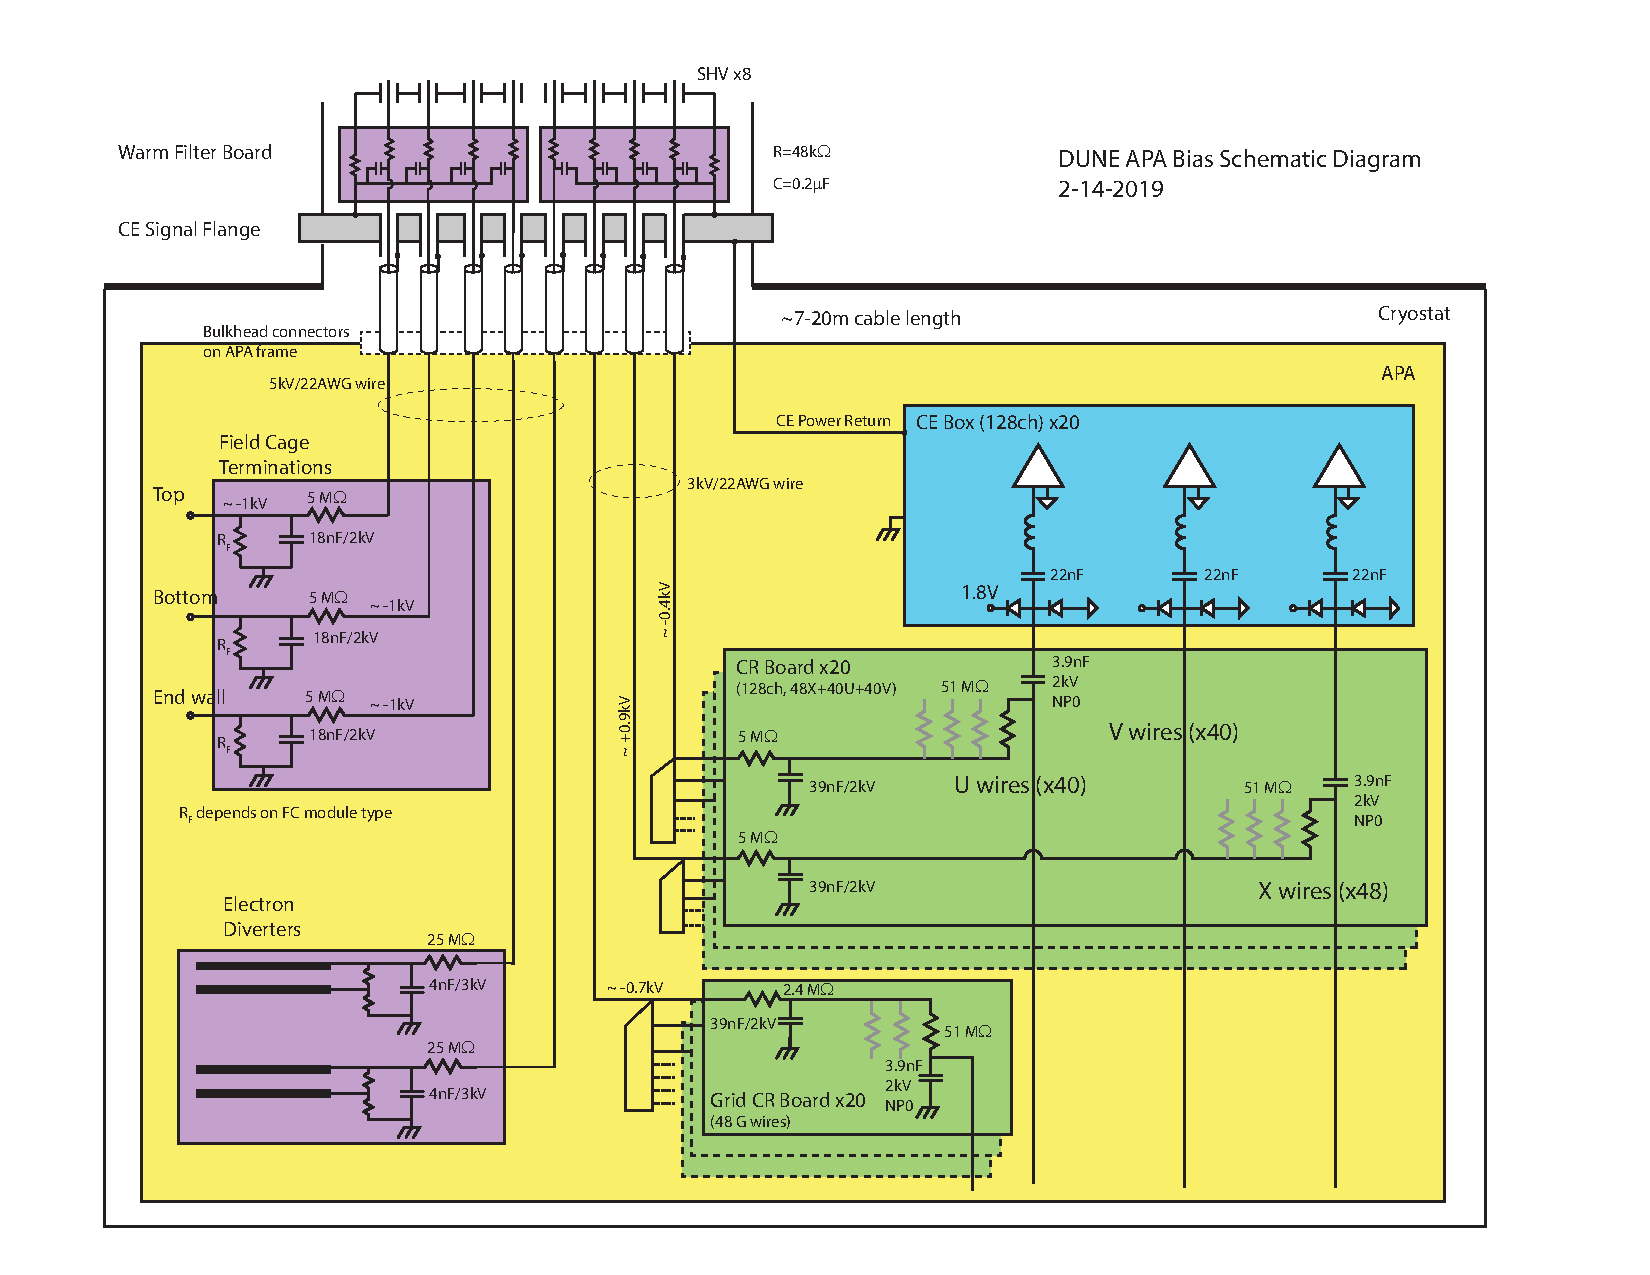
\includegraphics[width=0.8\linewidth]{sp-tpcelec-cr-board.pdf}
\end{dunefigure}

Bias resistance values should be at least \SI{20}{\mega\ohm} to 
maintain negligible noise contributions. The higher value helps 
achieve a longer time constant for the high-pass coupling networks.
Time constants should be at least \num{25} times the electron 
drift time so that the undershoot in the digitized waveform
is small and easily correctable. %However, leakage currents can develop on \dwords{pcb} that are exposed to high voltages over extended periods. If the bias resistors are much greater than \SI{50}{\mega\ohm}, leakage currents may affect the bias voltages applied to the wires.
As discussed in Section~\ref{sec:crboards},
the bias resistance value is \SI{51}{\mega\ohm}, while the 
\dword{dc}-blocking capacitors on each wire have a value of
\SI{3.9}{nF}. This gives a time constant of \SI{0.2}{s} that
is much larger than the drift time for electrons from tracks
passing near the cathode ($\sim\SI{2.3}{ms}$).

The bias-voltage filters are RC low-pass networks. Resistance 
values should be much smaller than the bias resistances to control 
cross-talk between wires and limit the voltage drop if any of the 
wires becomes shorted to the \dword{apa} frame. As discussed
in Section~\ref{sec:crboards}, these resistors are 
\SI{5}{\mega\ohm}, while the bias filter capacitors are \SI{39}{nF}.

%%%%%%%%%%%%%%%%%%%%%%%%%%%%%%%%%%%
\subsection{Front End Motherboard}
\label{sec:fdsp-tpcelec-design-femb}

Each \dword{apa} is instrumented with \num{20} \dwords{femb}.
The \dwords{femb} plug into the \dword{apa} \dword{cr} boards, 
making the connections from the wires to the charge amplifier 
circuits as short as possible. Each \dword{femb} receives signals 
from \num{40} $U$ wires, \num{40} $V$ wires, and \num{48} $X$ wires.
The baseline \dword{femb} design contains eight \num{16}-channel 
\dword{larasic} chips, eight \num{16}-channel 
\dword{coldadc} \dwords{asic}, and two \dword{coldata} control and 
communication \dwords{asic} (see Figure~\ref{fig:ce-scheme}).
The \dword{femb} also contains regulators that produce the voltages 
required by the \dwords{asic} and filter those voltages, and 
a micro-electromechanical system oscillator that provides
a \SI{40}{MHz} reference to the \dword{coldata} \dword{pll}. The \dword{larasic} 
inputs are protected by an external series inductor and two 
diodes as well as the internal diode protection in the chip.

The \dword{pdsp} version of the \dword{femb} (which uses a single 
\dword{fpga} on a mezzanine card instead of two \dword{coldata} 
\dwords{asic}) is shown in Figure~\ref{fig:femb}. In the rest of
this section we describe the \dwords{asic} that will be installed
on the \dwords{femb} and discuss the procedure that will be 
followed to choose the \dword{asic} design %solution to be implemented for 
to implement in the %\dword{dune} 
\dword{spmod}. % construction. 
In addition to
describing \dword{larasic}, \dword{coldadc}, and \dword{coldata},
we also discuss two alternative solutions, one based on a 
\dword{cots} \dword{adc}, and one where the functionality of the
three \dwords{asic} is implemented in a single chip, \dword{cryo}.

\begin{dunefigure}
[The complete FEMB assembly as used in ProtoDUNE-SP]
{fig:femb}
{The complete \dword{femb} assembly as used in the \dword{pdsp} 
detector. The cable shown is the high-speed data, clock, and control cable.}
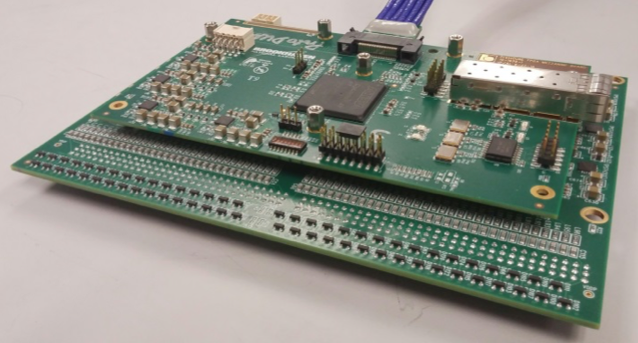
\includegraphics[width=0.6\linewidth]{sp-tpcelec-femb.png}
\end{dunefigure}

The functionality of the \dword{femb} for \dword{dune} will be
almost identical to that of \dword{femb} used in \dword{pdsp}.
The design will change slightly to accommodate the new \dwords{asic},
which will also entail changing the connections to the \dword{wib},
and changing the number of voltage regulators. In addition, the
connector for the control and data cold cables will be replaced
to address the issue observed in \dword{pdsp} that will be discussed
in Section~\ref{sec:fdsp-tpcelec-overview-lessons}. The new design,
shown in Figure~\ref{fig:femb-connector}, foresees the addition
of wings to the \dword{pcb} soldered to the cold cable, with 
standoffs to ensure the planarity of the connector
to the \dword{femb}, and a cutout in the \dword{pcb} to preclude %avoid
any stresses introduced by height variations.

\begin{dunefigure}
[Modified design of the cold data cable and of the FEMB PCB]
{fig:femb-connector}
{Modified design of the cold data cable and of the \dword{femb} \dword{pcb}.}
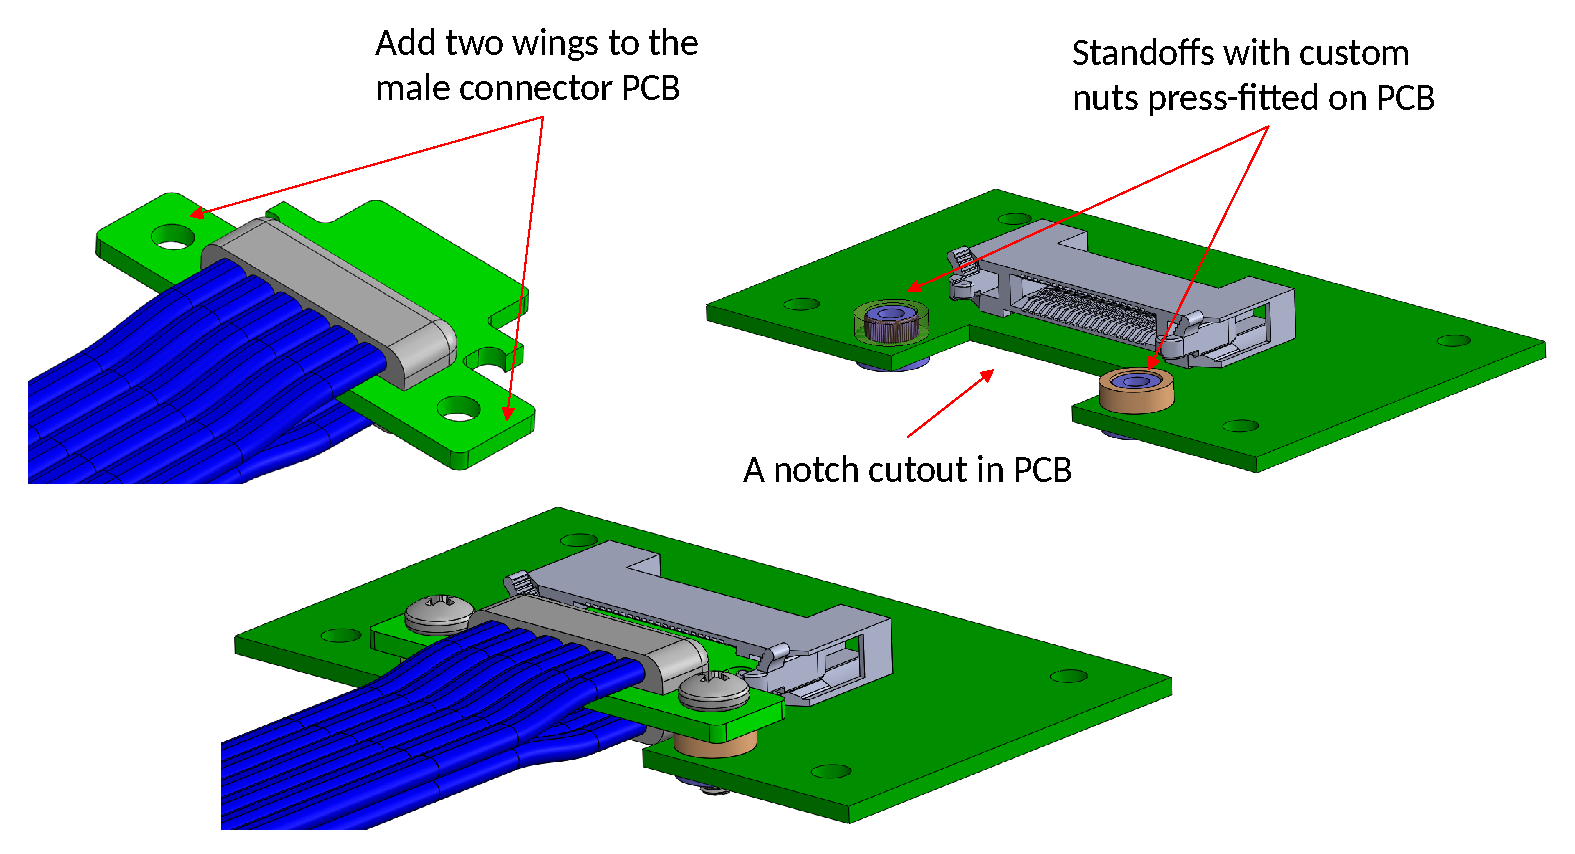
\includegraphics[width=0.9\linewidth]{sp-tpcelec-connector.pdf}
\end{dunefigure}

All the discrete components mounted on the \dword{femb} have been
characterized for operation in \dword{lar}. In some cases (resistors,
capacitors, diodes) the components used on the \dword{pdsp} \dword{femb}
belong to the same family of components already used for other boards
operating in cryogenic environment, namely the boards used for the 
ATLAS accordion \dword{lar} calorimeter, providing relevant information
on the lifetime of these components, that is discussed later in 
Section~\ref{sec:fdsp-tpcelec-qa-reliability}. There we also discuss
procedures for the measurement of the lifetime of discrete
components that have been adopted in recent years to demonstrate
that the \dword{tpc} electronics can survive in \dword{lar}. 
These types of measurements have been performed already for 
other neutrino experiments using the \dword{lar} \dword{tpc}
technology, while for the micro-mechanical oscillator we 
rely on characterizations performed by \dword{nasa}.

In the case of custom \dwords{asic}, appropriate steps must be taken prior 
to starting the layout of the chips. Both \dword{coldata} and 
\dword{coldadc} are implemented in the \dword{tsmc} \SI{65}{nm} \dword{cmos} 
process~\cite{TSMC65}. The designs were done using cold transistor models 
produced by Logix Consulting\footnote{Logix\texttrademark{} Consulting, http://www.lgx.com/.}.  Logix made measurements of 
\dword{fnal}-supplied \dword{tsmc} \SI{65}{nm} transistors at \lntwo 
temperature and extracted and provided to the design teams \dword{spice}~\cite{spice}
models valid at \lntwo temperature.  These models were used in 
analog simulations of \dword{coldata} and \dword{coldadc} subcircuits.  
In order to eliminate the risk of accelerated aging due to the hot-carrier
effect~\cite{Hot-electron}, no transistor with channel length
less than \SI{90}{nm} was used in either \dword{asic} design.
A special library of standard cells using \SI{90}{nm} channel-length 
transistors was developed by members of the University
of Pennsylvania and \dword{fnal} groups. Timing parameters were
developed for this standard cell library using the Cadence Liberate
tool\footnote{Cadence Liberate\texttrademark{}, \url{https://www.cadence.com/content/cadence-www/global/en_US/home/tools/custom-ic-analog-rf-design/library-characterization/liberate-characterization.html}. } 
and the Logix \dword{spice} models. With the
exception of the \dword{coldata} \dword{pll}, serializer, and
output driver, the digital sections of \dword{coldata} and
\dword{coldadc} were synthesized from Verilog code using this
standard cell library and the Cadence Innovus tool~\footnote{Cadence Innovus\texttrademark{}, \url{https://www.cadence.com/content/cadence-www/global/en_US/home/tools/digital-design-and-signoff/hierarchical-design-and-floorplanning/innovus-implementation-system.html}.}. 
Innovus was also used for the layout of the synthesized logic.
The design of the \dword{cryo} \dword{asic} and of \dword{larasic}
are implemented in the \dword{tsmc} \SI{130}{nm} and \SI{180}{nm} 
\dword{cmos} process~\cite{TSMC130,TSMC180}, respectively. 
In the case of \dword{larasic}, 
the design uses models that were obtained by extrapolating the
parameters of the models provided by \dword{tsmc}, which are 
generally valid in the \SIrange{230}{400}{K}. In the case of the \dword{cryo}
\dword{asic}, cold transistor models were based on data taken at \dword{slac} with
\dword{tsmc}-produced \SI{130}{nm} transistors.

%%%%%%%%%%%%%%%%%%
\subsubsection{Front End \dword{asic}}
\label{sec:fdsp-tpcelec-design-femb-fe}

\dword{larasic}~\cite{DeGeronimo:2011zz} receives 
current signals from the \dword{tpc} sense wires and provides a way to 
amplify and shape the signals for downstream signal digitization. 
\dword{larasic} has \num{16} channels and is implemented 
using the \dword{tsmc} \SI{180}{nm} \dword{cmos} process~\cite{TSMC180}. It 
integrates a band-gap reference to generate all the internal bias 
voltages and currents. This guarantees high stability of the operating 
point over a wide range of temperatures, including cryogenic temperatures. 
The channel schematic of \dword{larasic} is shown in 
Figure~\ref{fig:feasic1}. 

\begin{dunefigure}
[FE ASIC channel schematic]
{fig:feasic1}
{Channel schematic of \dword{larasic}, which includes a 
dual-stage charge amplifier and a \num{5}$^{th}$ order semi-Gaussian 
shaper with complex conjugate poles. Circuits in red circles are 
programmable to allow different gain and peaking time settings.}
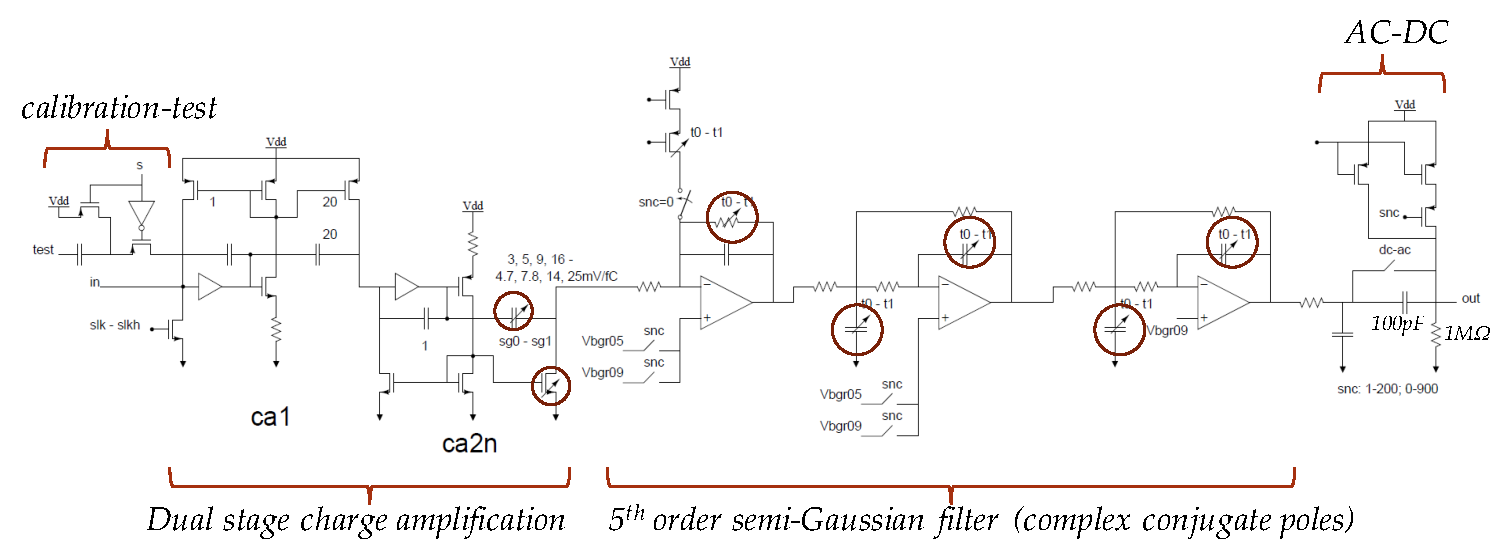
\includegraphics[width=0.99\linewidth]{sp-tpcelec-feasic-channelschematic.pdf}
\end{dunefigure}

Each \dword{larasic} channel has a dual-stage charge amplifier 
and a \num{5}$^{th}$ order semi-Gaussian shaper as an anti-aliasing 
filter for the \dword{tpc} signals. It has programmable gain 
selectable, at the \dword{asic} level, from one of \num{4.7}, \num{7.8}, \num{14}, or \SI{25}{mV/fC}
(corresponding to full-scale charge of \num{1.9e6}, \num{1.1e6}, \num{625e3}, 
and \SI{350e3}{$e^-$}), programmable peaking time selectable from one of 
\num{0.5}, \num{1}, \num{2}, and \SI{3}{$\mu$s}, and programmable 
baseline for operation with either the collection ($\sim$\SI{200}{mV}) 
or the induction ($\sim$\SI{900}{mV}) wires. The design of
\dword{larasic} has been optimized for the capacitive
loads expected in the case of \dword{dune} (i.e. in the range \SIrange{170}{210}{pF}).
Each channel has an 
option to enable the output monitor to probe the analog signal, and 
an option to enable a high-performance output driver that can be 
used to drive a long cable. 

Each \dword{larasic} channel has a built-in charge calibration 
capacitor that can be enabled or disabled through a dedicated register. 
Measurements of the injection capacitance have been performed using an 
external precisely calibrated capacitor. These measurements show that
the calibration capacitance is extremely stable against temperature variations, 
changing from \SI{184}{fF} at room temperature to 
\SI{183}{fF} at \SI{77}{K}. This result and the measured stability of 
the peaking time demonstrate the high stability of the passive 
components as a function of temperature. Channel-to-channel and 
chip-to-chip variation in the calibration capacitor are typically 
less than \num{1}\%. The variations of the calibration capacitors
could be characterized prior to the beginning of \dword{dune}
data taking, using the \dword{qc} process, discussed in
Section~\ref{sec:fdsp-tpcelec-production-qc}.

Shared among the \num{16} channels in \dword{larasic} are 
the digital interface, programming registers, a temperature monitor, 
and a band-gap reference monitor. It is also possible to enable \dword{ac} 
coupling as mitigation of baseline variations induced by vibrations
of the \dword{apa} wire, a programmable input bias current 
selectable from one of \num{0.1}, \num{0.5}, \num{1}, or \SI{5}{nA}, 
as well as a programmable pulser generator with a \num{6}-bit 
\dword{dac} for calibration. The possibility of configuring various
parameters controlling the \dword{fe} amplifier (gain, shaping time,
baseline) has allowed \dword{pdsp} to reduce the impact of the
saturation effect discussed in Section~\ref{sec:fdsp-tpcelec-overview-lessons}, 
at the cost of a reduction in dynamic range.

The power dissipation of \dword{larasic} is about \SI{5.5}{mW} 
per channel at \SI{1.8}{V} supply voltage when the output buffer is
disabled (the output buffer is required only for transmitting analog
signals over long distances; it is not needed when \dword{larasic}
is mounted close to the \dword{adc} on the \dword{femb}).
The \dword{asic} is packaged in a commercial, fully encapsulated 
plastic \num{80} pin \dword{qfp}. Figure~\ref{fig:feasic2} shows the 
response of \dword{larasic} for all gains and peaking times 
and both baselines. Note that the gain is independent of the peaking 
time; the same amount of charge, in the impulse approximation, produces 
the same peak voltage signal regardless of the peaking time.

\begin{dunefigure}
[FE ASIC response and layout]
{fig:feasic2}
{Response of \dword{larasic} for four gains, four peaking times, 
and both baseline values (left, the time distance between the positive
and negative pulse for the induction wires has been exaggerated
for clarity reasons); layout of \num{16}-channel
\dword{larasic} version P3, where revisions with reference to version 
P2 are highlighted in yellow boxes (right).}
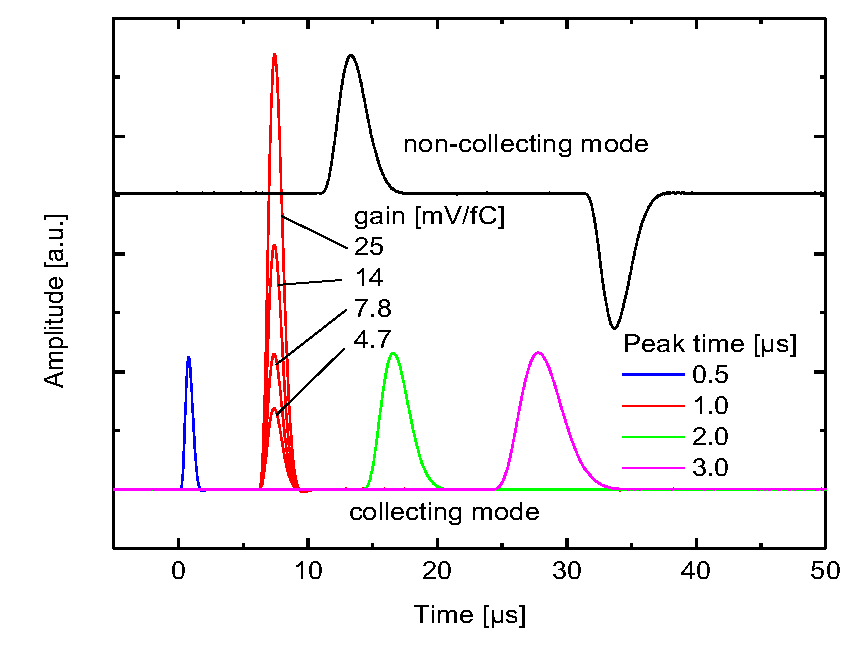
\includegraphics[width=0.53\linewidth]{sp-tpcelec-feasic-response.pdf}
\hspace{6mm}
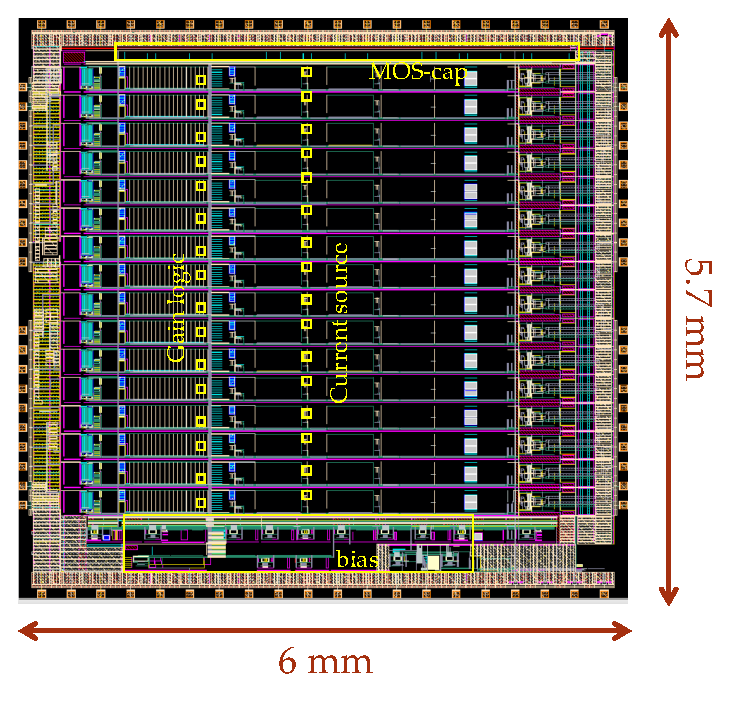
\includegraphics[width=0.42\linewidth]{sp-tpcelec-feasic-layout.pdf}
\end{dunefigure}

Prototype version P2 \dword{larasic} chips have been evaluated and 
characterized at room temperature and \lntwo (\SI{77}{K}) temperature. 
\num{960} P2 chips, totaling \num{15,360} channels, 
have been used to instrument six \dword{pdsp} \dword{apa}s successfully. 
Excessive stress in the package of \dword{larasic} at cryogenic 
temperature causes \dword{fe} channels to have a non-uniform baseline in 
collection mode, while the baseline \dword{dc} voltage in induction mode 
is uniform. A new prototype, version P3, was fabricated in March 2018 
to address this issue by making \dword{dc} circuits for the collection mode 
similar to the induction mode. At the same time, the default gain
setting was changed to \SI{14}{mV/fC}. The layout of P3
\dword{larasic} is also shown in Figure \ref{fig:feasic2}, with modifications 
highlighted in yellow boxes. The P3 \dword{larasic} chips were 
received and evaluated in September 2018. We have verified that with
the new design the \dword{fe} channels have a uniform baseline when
operated in the collection mode, and that the new default gain setting
is working properly.

P3 \dword{larasic} will be further evaluated on \dwords{femb} 
in various integration test stands for performance studies, including 
the \num{40}\% \dword{apa} at \dword{bnl}, the \dword{iceberg} \dword{tpc} 
at \dword{fermilab} and the seventh \dword{protodune} \dword{apa} 
in the cold box at \dword{cern}. Analysis of the \dword{pdsp} data
has highlighted a saturation problem in the design of the P2 \dword{larasic}
that we have observed also in bench tests of the P3 version. This problem,
discussed in detail in Section~\ref{sec:fdsp-tpcelec-overview-lessons}),
will be addressed in the design of the next version of \dword{larasic}, P4,
for which we are also planning to implement a single-ended-to-differential
converter as an interface to the recently developed \dword{coldadc}.
The plan for solving the saturation problem in \dword{larasic} is discussed 
in Section~\ref{sec:fdsp-tpcelec-overview-remaining}.

%%%%%%%%%%%%%%%%%%
\subsubsection{\dword{coldadc} \dword{asic}}
\label{sec:fdsp-tpcelec-design-femb-adc}

\dword{coldadc} is a low-noise \dword{adc} \dword{asic} designed to digitize
\num{16} input channels at a rate of $\sim\SI{2}{MHz}$, as required for the
\dword{dune} \dword{spmod}. \dword{coldadc} was designed to operate with 
an external \SI{64}{MHz} clock and an external \SI{2}{MHz} digitization clock.
The \SI{2}{MHz} clock is aligned on the rising edge of one of
the \SI{64}{MHz} transitions, as discussed in Section~\ref{sec:fdsp-tpcelec-design-femb-coldata}.
For the remainder of this section we assume that the main clock is operating
at \SI{64}{MHz}, but in the \dword{dune} \dword{spmod} this external clock will operate at \SI{62.5}{MHz}
as discussed in Section~\ref{sec:fdsp-tpcelec-design-femb-coldata}. 
\dword{coldadc} is implemented in the \dword{tsmc}
\SI{65}{nm} \dword{cmos} technology and has been designed by a team of engineers
from \dword{lbnl}, \dword{bnl}, and \dword{fnal}.  The \dword{asic} uses a conservative,
industry-standard design including digital calibration.  Each \dword{coldadc}
receives \num{16} voltage outputs from a single \dword{larasic} chip.  The voltages
are buffered, multiplexed by \num{8}, and input to two \num{15}-stage pipelined \dwords{adc}
operating at \SI{16}{MHz}. The \SI{16}{MHz} clock is generated internally in
\dword{coldadc} and shares its rising edge with the \SI{2}{MHz} clock. 
The \dword{adc} uses the well-known pipelined architecture
with redundancy~\cite{PipelinedADC}.  Digital logic is used to correct non-linearity
introduced by non-ideal amplifier gain and offsets in each pipeline
stage~\cite{CalibrationCorrection}, and an automatic calibration procedure is
implemented to determine the constants used in this logic.  The \dword{adc} produces
\num{16}-bit output which is expected to be truncated to \num{12} bits.

The \dword{adc} is highly programmable to optimize performance at different
temperatures.  Many circuit blocks can be bypassed, allowing the performance 
of the core digitization engine to be evaluated separately from the ancillary 
circuits. A block diagram of the chip is shown in Figure~\ref{fig:COLDADC_Block_Diagram}. 
Each of the major blocks is described below.

\begin{dunefigure}
[ColdADC block diagram]
{fig:COLDADC_Block_Diagram}
{\dword{coldadc} block diagram}
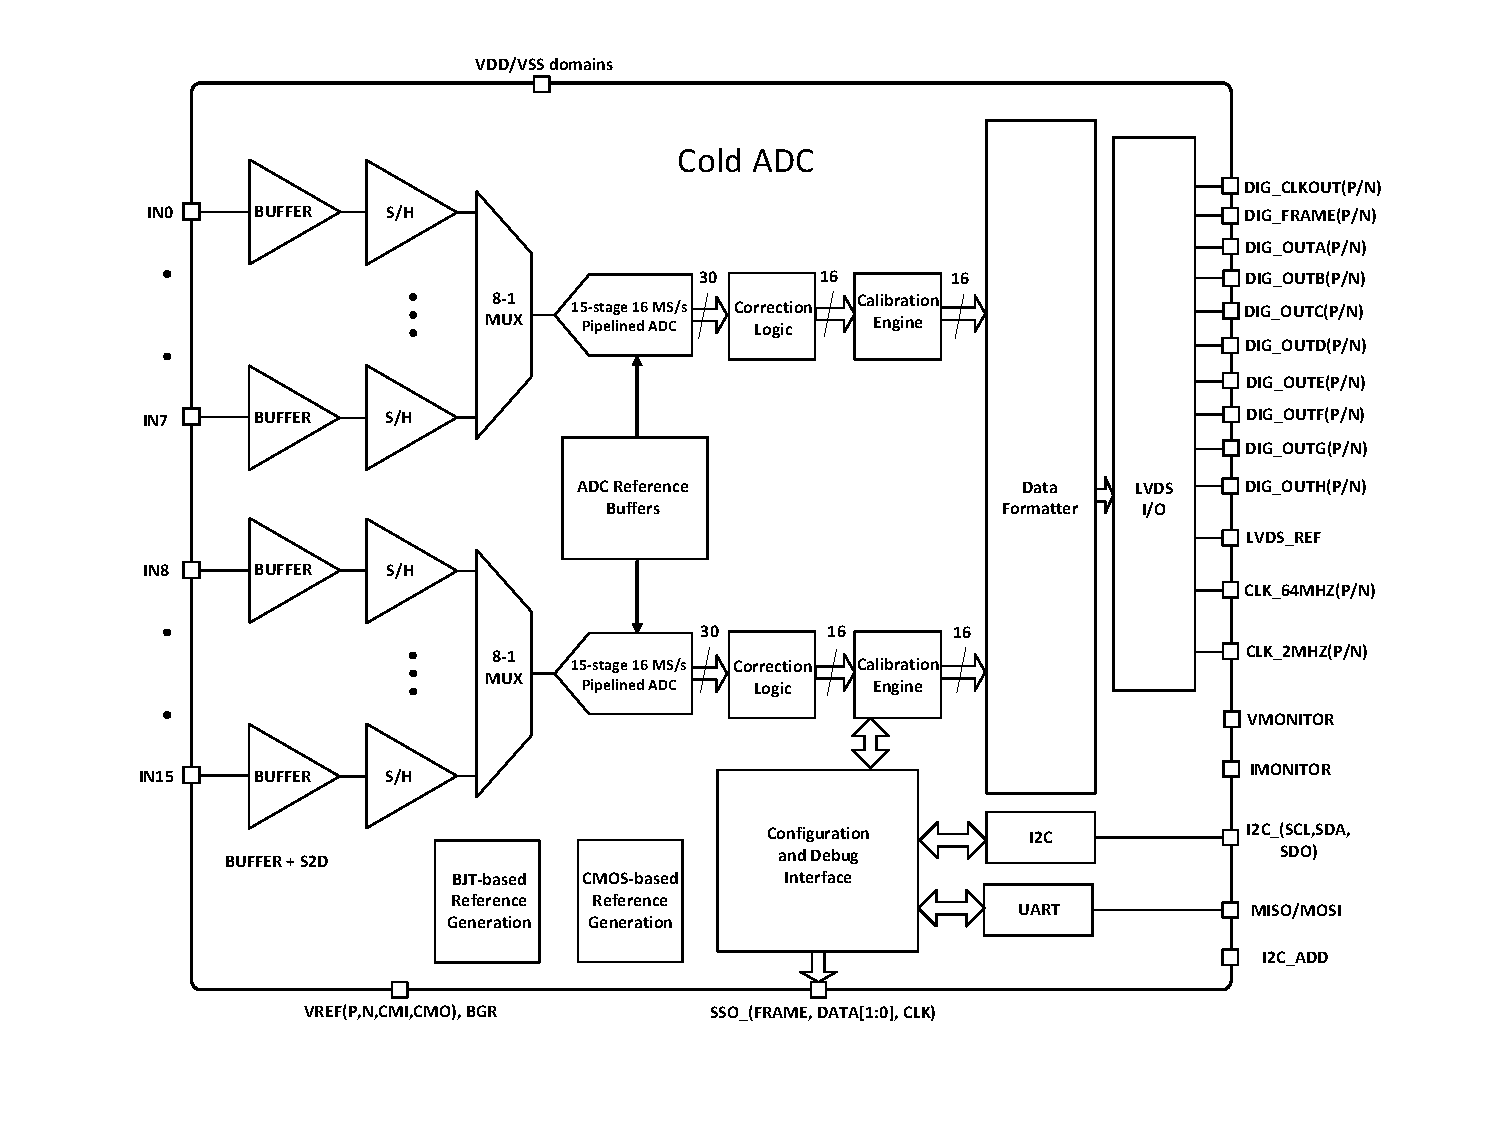
\includegraphics[width=0.8\linewidth]{sp-tpcelec-COLDADCblockdiagram.pdf}
\end{dunefigure}

All required reference voltages and currents are generated on-chip by programmable
circuit blocks. Independently adjustable bias voltage levels and currents are provided for the
input buffers, sample-and-hold amplifiers, \dwords{adc}, and \dword{adc}
reference buffers.
The most accurate reference voltage circuit is a band-gap reference
based on a \dword{pnp} transistor.  However, measurements made at \dword{bnl} and
\dword{lbnl} of a large \dword{pnp} transistor indicate that the foundry-provided \dword{spice} model
does not adequately describe the device operation at \lar temperature.  Thus,
a \dword{cmos}-based voltage reference has also been included in \dword{coldadc}.
As discussed below, bench tests of \dword{coldadc} prototypes show that both reference blocks 
perform well and meet requirements.

\dword{coldadc} has four possible ways to interface with \dword{larasic}.  It
can accept either single-ended inputs (provided by existing \dword{larasic}
chips) or differential inputs (foreseen for the future \dword{larasic} P4 upgrade).
In either case, it is also possible to bypass the input buffers and apply the inputs directly
to the sample-and-hold amplifiers. The role of the input buffers is to present a well-defined
and easy-to-drive load to \dword{larasic}.  The sample-and-hold amplifiers are separated
into two groups of eight. They sample the waveform at the rising edge of the
(\SI{2}{MHz}) sampling clock. The \SI{16}{MHz} clock is then
used to clock an \num{8}-to-\num{1} multiplexer that presents eight samples in 
turn to one of the two \dword{adc} pipelines.

\begin{dunefigure}
[Circuit blocks in each ADC pipeline stage]
{fig:pipelinestage}
{Circuit blocks in each \dword{adc} pipeline stage. MUX selects one of three values
as the digitized output of the current stage and presents it to the ADD circuit, which 
adds it to the result calculated by previous pipeline stages.
SHA is a sample-and-hold, and
ADCS and DASC are low resolution 1.5 bit analog-to-digital and digital-to-analog 
subconverters, respectively.}
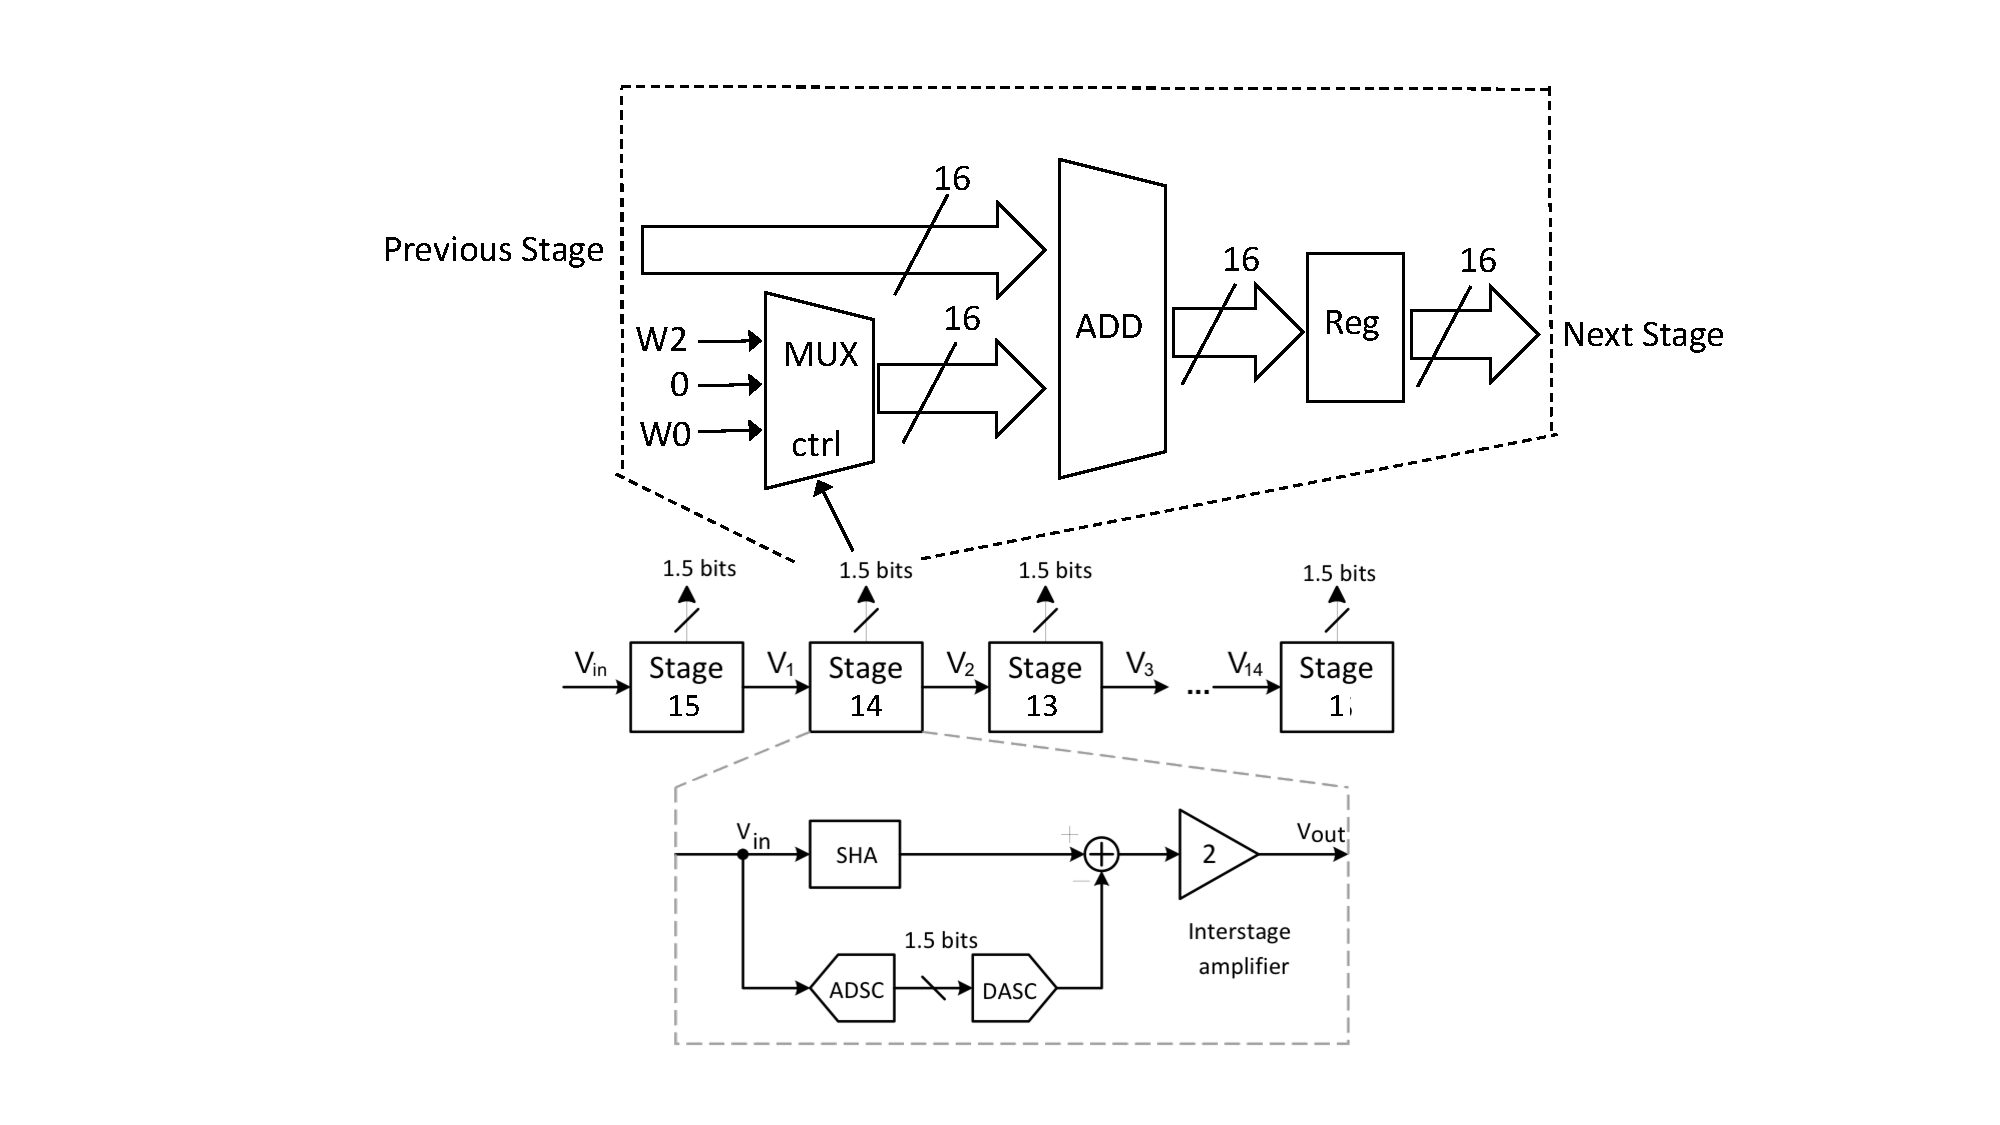
\includegraphics[width=0.9\linewidth]{sp-tpcelec-Pipelinestage.pdf}
\end{dunefigure}

A block diagram of an \dword{adc} pipeline is shown in
Figure~\ref{fig:pipelinestage}. Each of the \num{15} stages contains a low-resolution
\num{1.5}-bit analog-to-digital subconverter containing two comparators, a
\num{1.5}-bit digital-to-analog subconverter that produces a voltage based on
the two comparator outputs, an analog subtractor, a sample-and-hold amplifier,
and a gain stage (with a nominal gain of two). The transfer function of
each stage is identical and is shown in Figure~\ref{fig:ADCXFERFN} along with
the nominal ``weights'' (W$_0$ and W$_2$) that are added to form the output of the
pipeline. Each pipeline stage makes a three-level coarse decision based on the
analog input voltage, selects one of three digital ``weights'' to be added to the
results of previous stages, and passes a voltage to the next stage that is
proportional to the difference between the input voltage and the voltage
corresponding to the digital output of the stage.  Because the stages are
weighted by a factor of two, but have three possible digital results, there is
redundancy between stages that makes the final result independent of errors in
the comparator thresholds (up to $\pm V_r/4$ where the stage range is
$[-V_r,V_r]$).  An ``error'' in the output of one stage is corrected in subsequent
stages (usually the next stage).  In order to take advantage of this redundancy
provided by the pipelined architecture it is necessary to include at least one
``extra'' stage in the pipeline.  The \dword{coldadc} pipelined \dwords{adc} are
implemented as \num{15}-stage pipelines.

\begin{dunefigure}
[ADC stage transfer function]
{fig:ADCXFERFN}
{\num{1.5}-bit stage transfer function and digital output. The voltage 
range of the \dword{adc} as a whole, and of each individual stage 
is $[-V_r,V_r]$.  Note that the voltage passed to the subsequent 
stage will not exceed the stage range even if a comparator threshold 
is wrong by up to $V_r/4$.}
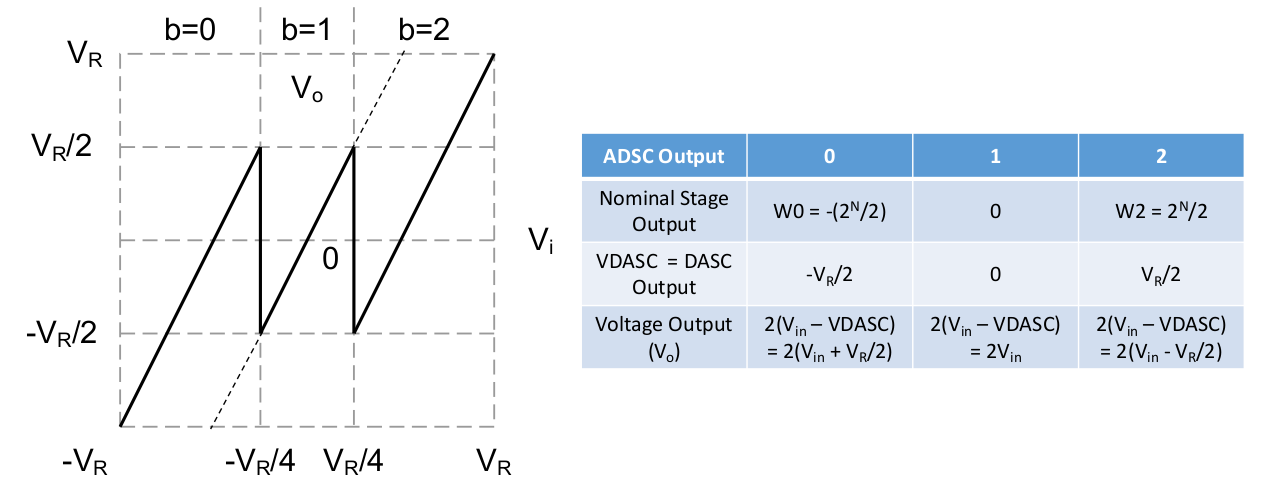
\includegraphics[width=0.90\linewidth]{sp-tpcelec-ADCXFERFN.png}
\end{dunefigure}

The calibration logic allows the correction of errors caused by imperfections
in the voltage that are passed from one stage to the next.  These imperfections
arise from errors in each stage corresponding to $\pm V_r/2$ from the resistive
dividers and non-ideal effects in the gain and offset of the interstage amplifiers.
The calibration procedure relies on the fact that the required precision is easily
satisfied by the last stages of the pipeline.
The number of stages to be calibrated (maximum \num{7}) is set by a programmable
register.  An iterative calibration procedure is used.  Starting with the least
significant stage to be calibrated, the input to the stage is set to the threshold
levels of $\pm V_r/4$ and the normal comparator outputs are overridden
and forced first to \num{1} and then to \num{0}.  The lower stages of the \dword{adc} digitize
the analog value output from the stage being calibrated and the difference between
the \dword{adc} output when the comparator is forced to \num{1} and the \dword{adc}
output when the comparator is forced to \num{0} is calculated.  These two differences
(W$_0$ expressed as a negative number and W$_2$ expressed as a positive number) are
stored and used as two of the three possible digital outputs of the stage being
calibrated (the third possible output being \num{0}).  This procedure is then repeated
for the next most significant pipeline stage until stage \num{15} has been calibrated.

The number of \dword{adc} bits that are useful depends on the effective
noise of the various subcircuits of the \dword{adc}.  The noise of the first few
pipeline stages (associated with the most significant bits) contributes more
heavily than subsequent stages.  For this reason, the first stages are designed
to be larger, lower noise, and to require more power than later stages. The capacitance
is reduced by a factor of two, relative to that of the sample-and-hold, for each
of the first three stages, and then kept constant. The total
effective noise expected is \SI{\sim130}{$\mu$V}-\dword{rms}.  This is similar to the
quantization error of an ideal \num{12}-bit \dword{adc} with a voltage range of
\SI{1.5}{V} (slightly larger than the output range of \dword{larasic}, \SIrange{0.2}{1.6}{V})
for which the bin width is \SI{366}{$\mu$V} and the quantization
error is \SI{\sim106}{$\mu$V}.

In normal operation, each pipelined \dword{adc} passes a \num{16}-bit result to the
data formatter on the rising edge of the \SI{16}{MHz} clock.  The data formatter
separates the two \num{16}-bit words into eight \num{4}-bit nibbles and serializes the
nibbles for output (most significant bit first) at \SI{64}{MHz}.   An output
clock and a frame marker are also generated.  The frame marker indicates the most
significant bit in each nibble of the first of eight channels digitized by one
of the \dword{adc} pipelines in each \SI{2}{MHz} sample period.  The output data
is generated on the falling edge of the output clock and is latched by the
\dword{coldata} \dword{asic} using the rising edge of the same clock.  

A second
mode of operation is included for debugging purposes.  In this mode, \num{2}-bit raw
stage results from each of the \num{15} stages of one of the two pipelines are formatted
into the most significant \num{15} bits of two \num{16}-bit words, broken into nibbles, and
output in the same manner as normal data.

Ten differential output drivers are used for the \SI{64}{MHz} output clock, frame
marker, and \dword{adc} data. The output drivers source and sink a current whose
value can be digitally controlled. The minimum current is \SI{165}{$\mu$A},
which corresponds to approximately \SI{3}{mV} peak-to-peak with \SI{100}{$\Omega$}
termination. Seven additional levels spaced by \SI{275}{$\mu$A} can be selected.
The maximum current is \SI{2.07}{mA}, about \num{2/3} of the \dword{lvds} standard of
\SI{3.5}{mA}.

The operation of \dword{coldadc} is controlled by a number of \num{8}-bit registers.
These registers can be written to and read back using either an \dword{i2c}
interface~\cite{bib:I2C} or a \dword{uart}. \dword{coldata} will use the \dword{i2c} interface. The
\dword{uart} is included in the first \dword{coldadc} prototype to facilitate chip testing
and for risk mitigation.

\dword{coldadc} was received at the end of January 2019.  Bench tests were performed at
\dword{bnl}, \dword{fnal}, and \dword{lbnl}. These tests used \dword{adc} chips mounted directly
on printed circuit boards, and were done at both room temperature and cryogenic temperature.
The tests concentrated first on functionality and later on performance.
A small number of problems were found during bench testing and will be described below. These problems
will not prevent system tests from being done with prototype \dword{coldadc} chips.

Both control interfaces (\dword{i2c} and \dword{uart}) operate as designed. All of the digital control
bits can be written and read. The \dword{lvds} I/O operates as designed and the drive current of the
\dword{lvds} can be selected as designed. The \dword{adc} pipeline functions as
designed, as does the data formatter. The automatic calibration logic does not work, but the pipelines 
can be calibrated off-chip using register-controlled debugging modes to force all of the steps of the 
calibration procedure. The sample-and-hold amplifiers and the multiplexer that connects the sample-and-hold 
outputs to the \dword{adc} pipelines operate correctly. Both the \dword{cmos} reference generation 
block and the band-gap reference block operate as designed, although a minor error in
a digital-to-analog converter in the band-gap reference block means that it must operate with the 
(nominally \SI{2.3}{V}) analog voltage set to \SI{2.7}{V}. Another error was discovered in the input 
buffer block. Level shifters intended to translate control bits in the \SI{1.2}{V} domain to the 
\SI{2.5}{V} domain were omitted. As a result, the \SI{1.2}{V} digital supply must be set to 
\SI{2.1}{V}. All of these design errors (including the auto-calibration failure) have been understood
and are easily corrected. Bench tests have proven that the \dword{coldadc} prototypes can be run at the 
required elevated voltage settings for many days without damage to the chips.

Performance measurements of \dword{coldadc} have also been done. The performance of many of 
the sub-circuits have been measured separately as well as the performance of the entire \dword{adc}.  
Here we present two measurements made at \lntwo temperature.

\fixme{Figure 4.11 will be replaced with a new one to be provided by Cheng-Ju Lin on 7/16.}

\begin{dunefigure}
[Static linearity of ColdADC]
{fig:ADCStaticLinearity}
{\dword{dnl} (top) and \dword{inl} distributions as a function of \dword{adc} code for \dword{coldadc}.}
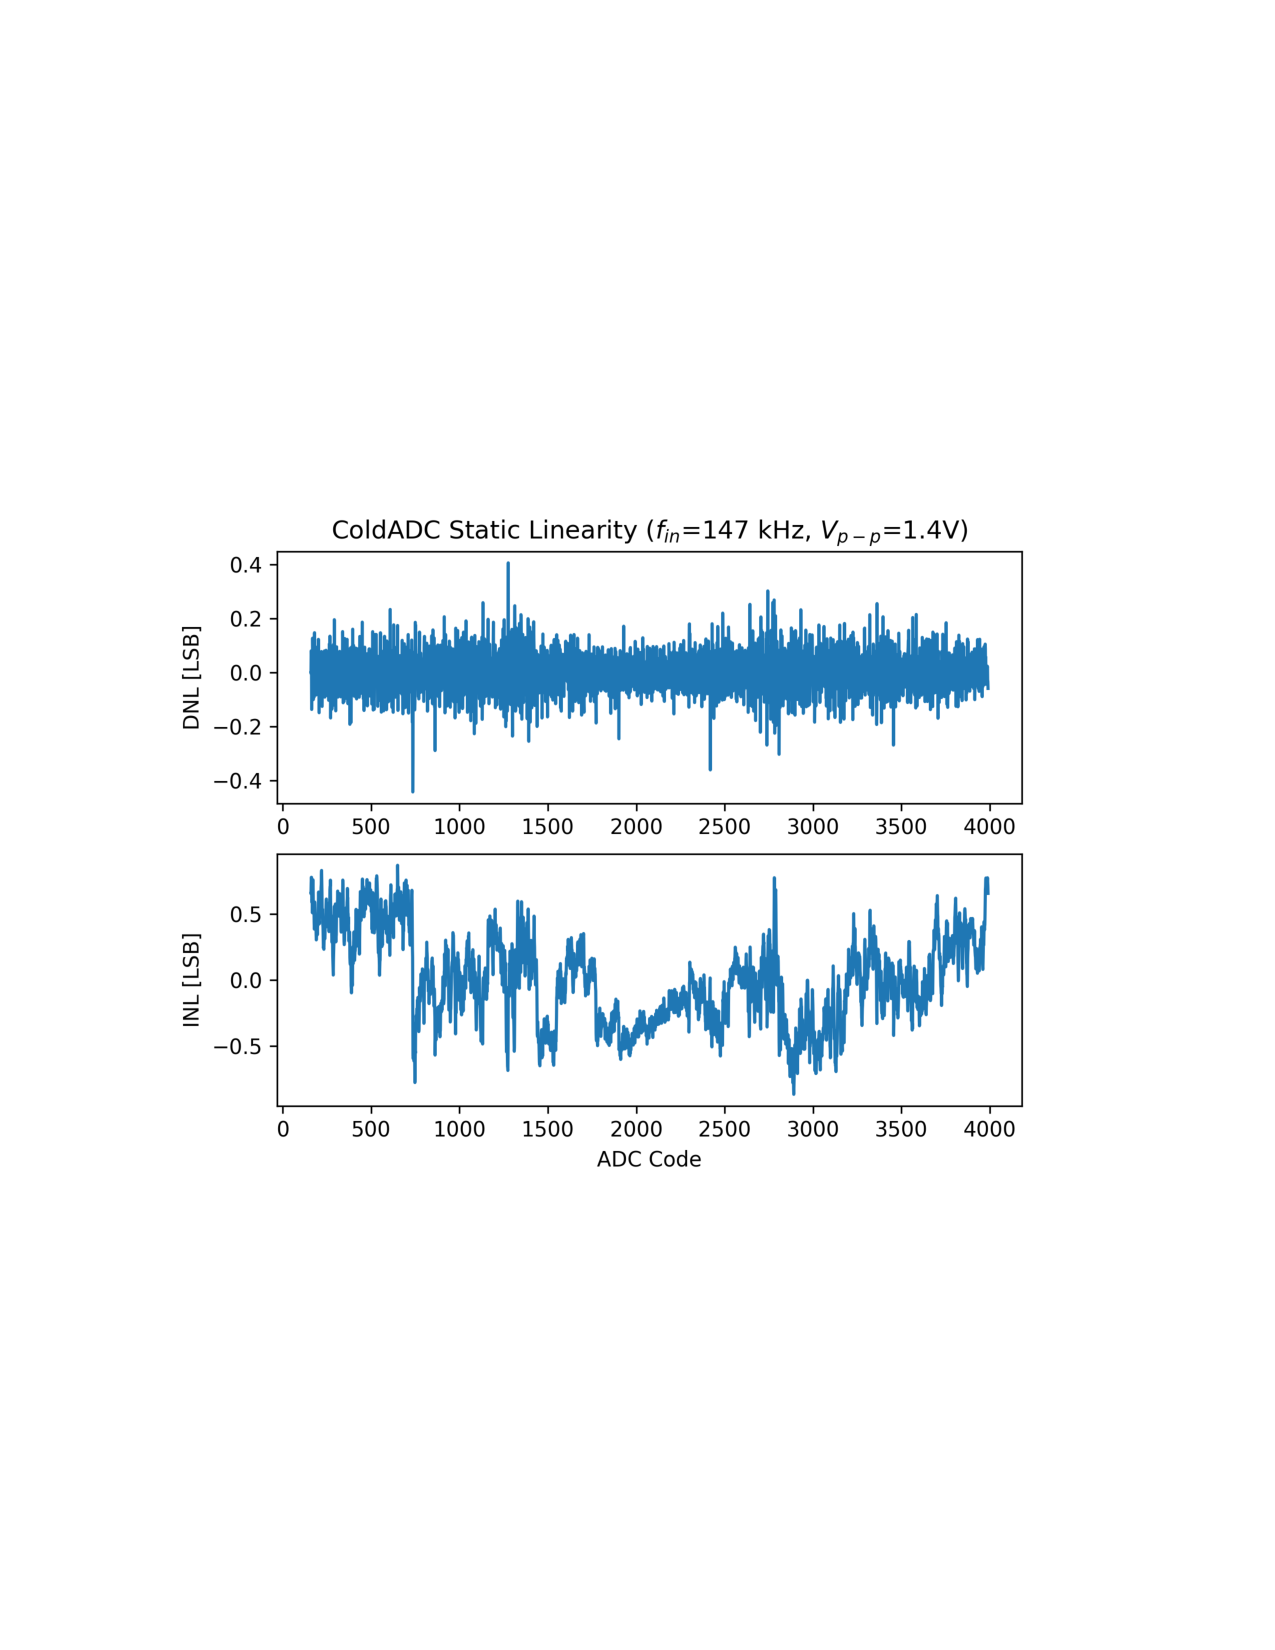
\includegraphics[width=0.9\linewidth]{sp-tpcelec-ADCStaticLinearity.pdf}
\end{dunefigure}

Static linearity was measured using a filtered sine wave input to the single-ended input buffer 
of one channel of \dword{coldadc}. The measured histogram of \dword{adc} codes was fit to the 
probability density function for a sine wave.  The deviations to the fit yields the \dword{dnl}
as a function of \dword{adc} code and the integral of \dword{dnl} is the \dword{inl}. These two
diistributions are shown in Figure ~\ref{fig:ADCStaticLinearity}, which was obtained using a sine 
wave of amplitude of \SI{1.4}{V} peak-to-peak (matching the \dword{larasic} dynamic range) and 
the nominal reference voltage settings (corresponding to a \SI{1.5}{V} dynamic range).

Dynamic linearity was also measured using a filtered sine wave. In this case, \dword{adc} codes were
collected for an integer number of sine wave cycles and a \dword{fft} was performed on the data. 
The \dword{sndr}, \dword{enob}, \dword{sfdr}, and the \dword{thd} were extracted from the \dword{fft}.
An example of the \dword{fft} is shown in Figure ~\ref{fig:ADCDynamicLinearity}, which was obtained 
using a sine wave of amplitude \SI{1.5}{V} (matching the full range of the \dword{adc}).
The extracted \dword{enob} is over 11, despite the non-linearity evident in 
Figure~\ref{fig:ADCStaticLinearity}, because the \dword{adc} noise is very low.
The dominant source of non-linearity has been demonstrated to be insufficient 
open-loop gain of the operational amplifier used in each pipeline stage. 
The design has already been modified to address this deficiency.

\begin{dunefigure}
[Dynamic Linearity]
{fig:ADCDynamicLinearity}
{Fourier transform of \dword{adc} codes collected with a coherently sampled sine wave input to a 
single-ended input buffer.}
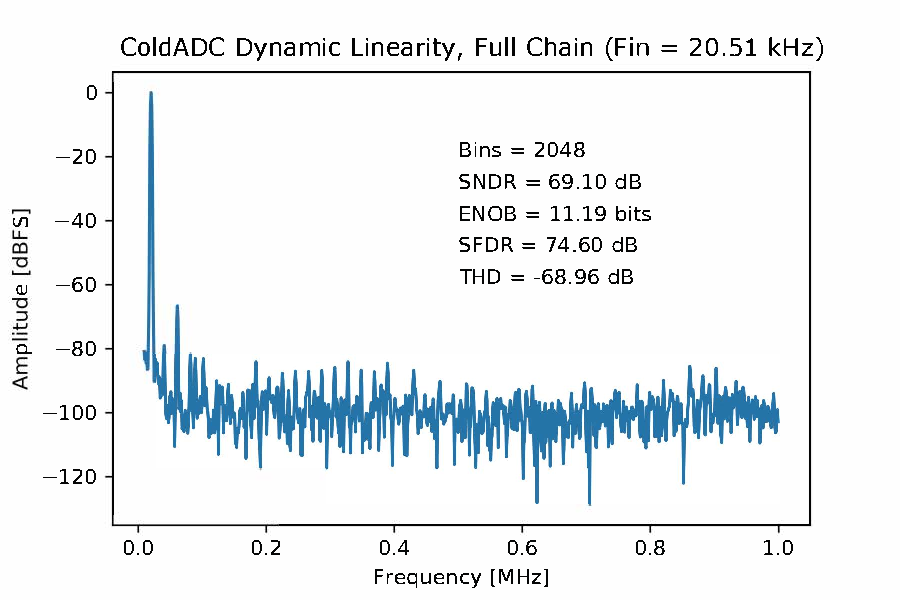
\includegraphics[width=0.9\linewidth]{sp-tpcelec-ADCDynamicLinearity.pdf}
\end{dunefigure}


%%%%%%%%%%%%%%%%%%
\subsubsection{COLDATA \dword{asic}}
\label{sec:fdsp-tpcelec-design-femb-coldata}

The \dword{coldata} \dword{asic} was designed by engineers from \dword{fermilab} 
and Southern Methodist University. It is responsible for all communications 
between the \dwords{femb} and the electronics located outside the cryostat. 
Each \dword{femb} contains two \dword{coldata} chips. \dword{coldata} receives 
command-and-control information from a \dword{wib}. Each \dword{coldata} provides 
clocks to four \dword{coldadc}s and relays commands to four \dword{larasic}s
and four \dword{coldadc}s to set operating modes and 
initiate calibration procedures.  Each \dword{coldata} receives data from four 
\dword{coldadc}s, merges the data streams, provides 8b/10b encoding, serializes 
the data, and transmits the data to the warm electronics over two \SI{1.28}{Gbps} 
links.  These links are driven by line drivers with programmable pre-emphasis. 
Figure~\ref{fig:coldata_block_diagram} is a block diagram of \dword{coldata}. 
The possibility of transmitting data from \dword{coldata} over a single 
\SI{2.56}{Gbps} link will be investigated in 2019, with the goal of further
reducing the number of cold cables that need to be routed through the
\dword{apa} frame, as discussed in Section~\ref{sec:fdsp-tpcelec-interfaces-apa}.

\begin{dunefigure}
[ColdDATA block diagram]
{fig:coldata_block_diagram}
{\dword{coldata} block diagram}
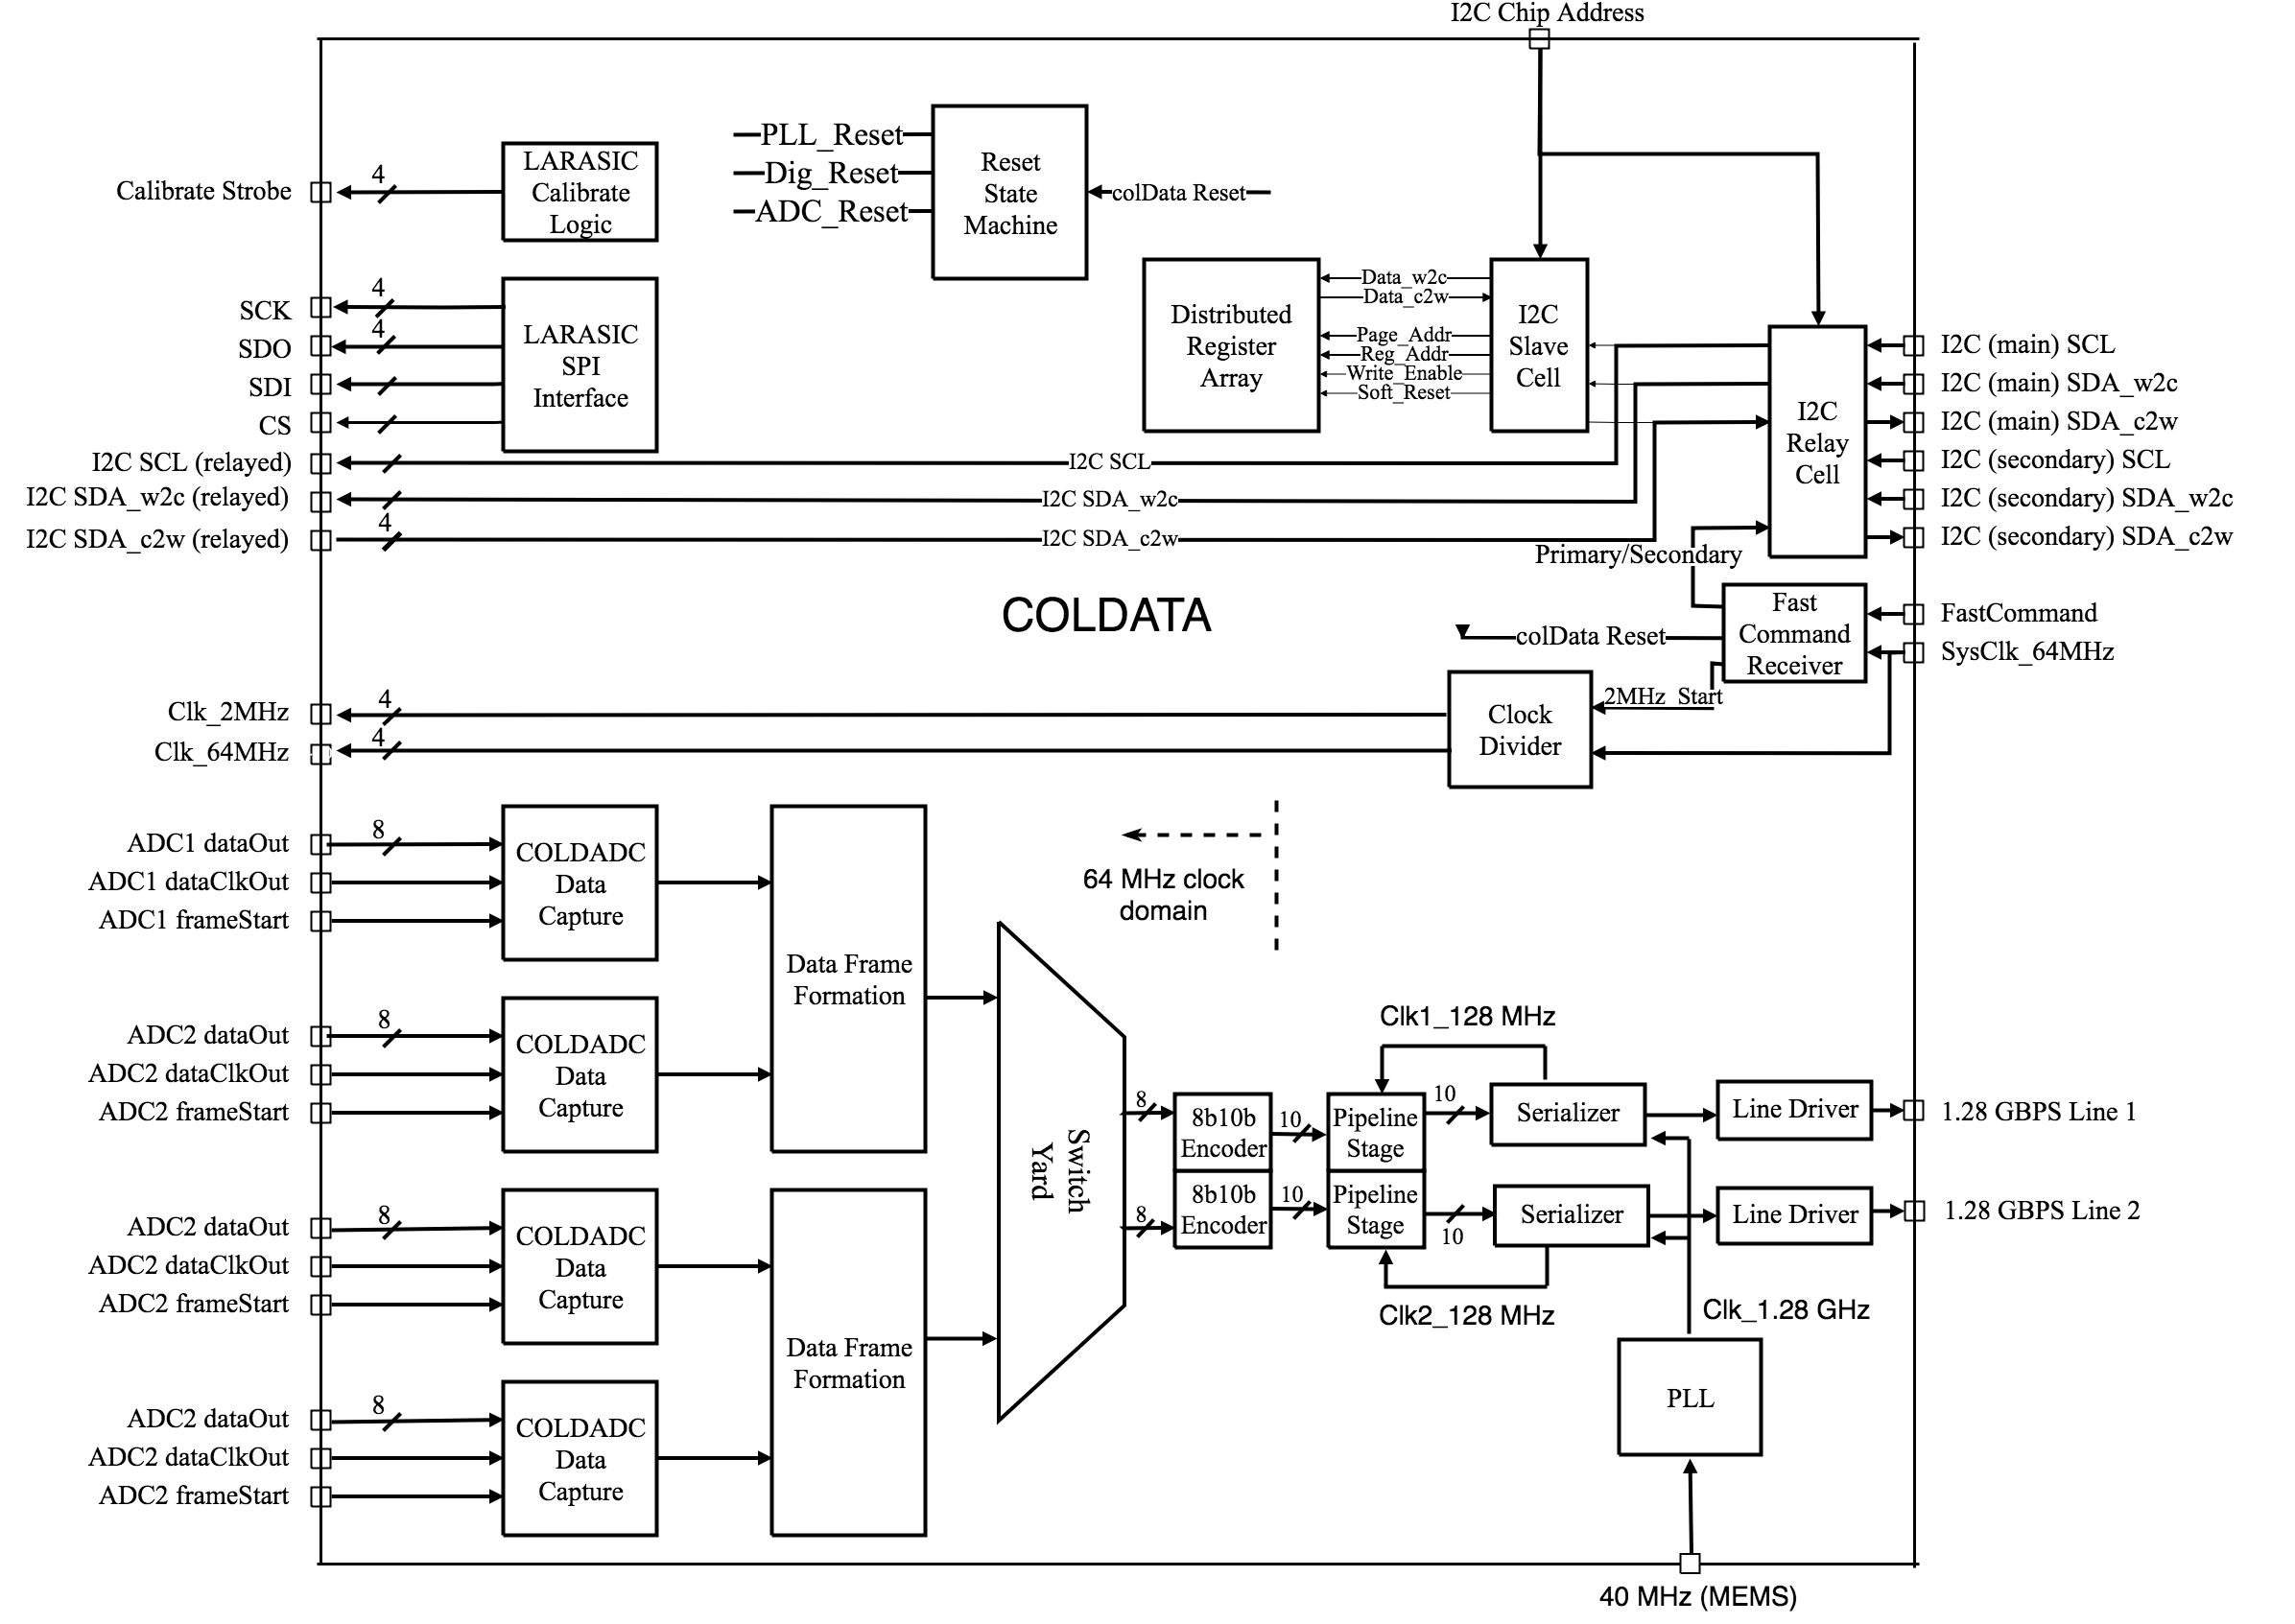
\includegraphics[width=0.99\linewidth]{sp-tpcelec-COLDATA-block-diagram.png}
\end{dunefigure}

The commands for the control of all the \dwords{asic} on a \dword{femb} are sent 
from a \dword{wib}  
using an \dword{i2c}-like~\cite{bib:I2C} protocol. While standard 
\dword{i2c} uses single-ended \dword{cmos} signals and a bidirectional data 
line, because of the long cables required between the \dword{wiec} and the 
\dwords{femb}, \dword{coldata} uses \dword{lv} differential pairs for both 
the \dword{i2c} clock and data. Separate point-to-point links are used for
data sent from warm-to-cold and for data sent from cold-to-warm.
In order to reduce the number of cables required, only one of the two 
\dword{coldata} chips on an \dword{femb} has its main \dword{i2c} interface 
directly connected to a \dword{wib}. That \dword{coldata} chip relays \dword{i2c} 
commands and data to the secondary \dword{coldata} chip and relays \dword{i2c} 
responses from the secondary \dword{coldata} to the \dword{wib}. 
Each  \dword{coldata} also relays \dword{i2c} commands and data sent from the 
\dword{wib} to one of the four \dword{coldadc} chips, and it relays data back to
the \dword{wib} from one of the  four \dword{coldadc} chips. 
The links on the \dword{femb} between \dword{coldata} 
chips and \dword{coldadc} chips use single-ended (\SI{2.25}{V}) \dword{cmos} 
signals, but the \dword{i2c} links are still non-standard since separate lines are
used for data transmission in the two directions.

The controls intended for the \dword{larasic} chips are interpreted 
inside \dword{coldata} and transmitted to the appropriate \dword{asic} using 
a \dword{spi}-like interface that uses single-ended (\SI{1.8}{V}) \dword{cmos} 
signals. The configuration registers in \dword{larasic} are configured to be 
loaded as a single-shift register. As data is shifted into \dword{larasic} on 
the \dword{mosi} line, bits from the other end of the shift register are shifted 
out on the \dword{miso} line. It is thus only possible to read \dword{larasic} 
configuration registers while writing new configuration data.

In addition to the configuration commands, \dword{coldata} 
receives a master clock and a fast command signal on a \dword{lv} 
differential pair from
the \dword{wib}. Currently the master clock is \SI{64}{MHz}, but it will be
changed to \SI{62.5}{MHz} to simplify the overall \dword{fd} \dword{spmod} 
synchronization, as already discussed in the case of \dword{coldadc}. The clock 
used for sampling the \dword{adc} is created inside
\dword{coldata} by dividing the master clock by \num{32}. The relative phase
of the \num{2} and the \SI{64}{MHz} clocks is set by an appropriate fast
command sent from the \dword{wib}.  Both the master clock and
the \dword{adc} sampling clocks are passed from \dword{coldata} to the four
\dword{coldadc} chips that it controls. Depending on the master clock frequency
the \dword{adc} will convert input data every \num{500} or \SI{512}{ns}, 
corresponding to a frequency of \num{2}, or \SI{1.95}{MHz}. Signals that must be
executed at a known time use the fast command line. \dword{coldata} 
uses the falling edge of the master clock to sample fast command bits as shown 
in Figure~\ref{fig:coldata_fast_command_timing}. All legal fast commands 
are \dword{dc} balanced. An ``alert'' pattern is used to establish the 8-bit 
fast-command word boundary. An ``idle'' pattern is used when no command is being 
sent. Four commands are defined: ``Edge,'' which moves the rising edge of the 
\dword{adc} sampling clock to coincide with the next rising edge of the 
master MHz clock; ``Sync,'' which zeros the \num{8}-bit timestamp that is the incremented 
on the rising edge of each \dword{adc} sampling clock; ``Reset,'' which resets 
\dword{coldata}; and ``ACT,'' the function of which is determined by an \num{8}-bit 
register that is programmed using the \dword{i2c} interface.  

\begin{dunefigure}
[ColdDATA fast command timing]
{fig:coldata_fast_command_timing}
{Fast command timing: the leading edges of the fast command and of the master 
clock are equal time when produced on the \dword{wib}. The fast-command bits 
are captured by \dword{coldata} on the falling edge of the master clock and 
shifted into a register on the next positive edge.}
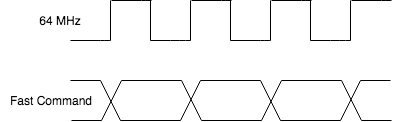
\includegraphics[width=0.4\linewidth]{sp-tpcelec-clocksandfastcommand.png}
\end{dunefigure}

\dword{coldata} receives digitized waveform data from 
four \dword{coldadc} \dwords{asic}. Each \dword{adc} presents its data on eight 
serial streams operating in parallel. Data from the \dwords{adc} is captured 
using the \dword{adc} dataClkOut signal  
(one per \dword{adc}) and the start of a 
sample period is indicated by the frameStart signal (one per \dword{adc}). 
Each \dword{adc} digitizes \num{16} channels of information and puts out \num{16} bits 
of data per channel. Information from two \dwords{adc} are merged by a Data 
Frame Formation block.  
The Data Frame Formation circuitry converts the two 
groups of sixteen \num{16}-bit words into one of three types of data frame. For normal 
data taking, either a \num{12}-bit format or a \num{14}-bit \dword{adc} format can be 
selected, discarding either the four or two lowest order bits. When the 
\num{12}-bit format is selected, a data frame consists of an 8b/10b command 
character (K28.2) and an \num{8}-bit time stamp, followed by \num{48} bytes of \dword{adc} 
data and two bytes of parity information. When the \num{14}-bit format is selected, 
a data frame consists of an 8b/10b command character (K28.3) and an \num{8}-bit time 
stamp, followed by \num{56} bytes of \dword{adc} data and two bytes of parity 
information. Two debugging frame formats are also defined. When the ``Frame-12 Test'' 
format is selected, a data frame consists of an 8b/10b command character 
(K28.0) and an \num{8}-bit time stamp, followed by \num{48} bytes of predefined data 
and two bytes of parity information. The final format is used when the 
\dwords{coldadc} are read out in debug mode. In this case, \num{30} bits of raw 
pipeline stage data are read out from one of the two pipelined \dwords{adc} 
in each \dword{coldadc} \dword{asic} and passed from \dword{coldadc} to 
\dword{coldata} using two \num{16}-bit frames. When the ``Frame-15'' format is 
selected, a \dword{coldata} output data frame consists of an 8b/10b command 
character (K28.6) and an \num{8}-bit time stamp, followed by \num{60} bytes of \dword{adc} 
data (\num{30} bytes from each \dword{coldadc}). No parity information is generated 
when this format is selected. This is to ensure that at least one idle 
character (K28.1) will be sent between each ``Frame-15.'' A series of 8b/10b 
command characters (K28.5) is sent at the end of each frame of \num{12}-bit or 
\num{14}-bit data to ensure synchronization of the high-speed links.

The serializers and output drivers operate asynchronously in a separate clock domain that
is not related to the master clock signal received from the \dword{wib}. Instead
they use clocks derived from a \SI{40}{MHz} micro-electromechanical
system oscillator on the \dword{femb}. A single \dword{pll} generates a 
\SI{1.28}{GHz} clock for both serializers and output drivers. The \num{10}-bit
serializers are implemented using two \num{5}:\num{1} multiplexers (clocked at \SI{128}{MHz}) 
followed by a single \num{2}:\num{1} multiplexer (clocked at \SI{640}{MHz}). Each serializer 
derives the \SI{640}{MHz} and \SI{128}{MHz} clock from the \SI{1.28}{GHz} 
clock provided by the \dword{pll} and provides its \SI{128}{MHz} clock to 
the Data Frame Formation block, which uses it at the output stage of a 
clock-domain-crossing \dword{fifo}. A link synchronization sequence of 8b/10b 
command characters (K28.5) is used when the link is reset to establish the 
boundary between \num{10}-bit ``words.'' Idle characters (K28.1) are inserted 
by the Data Frame Formation block when no data is ready for serialization 
(between data frames). The \SI{1.28}{Gbps} output drivers include programmable 
pre-emphasis. The pre-emphasis is achieved using a combination of a voltage 
mode circuit at the input to the current mode driver and current mode 
pre-emphasis integrated into the driver circuit. Measurements were made 
of the insertion loss (``S parameters'') as a function of frequency using
\num{25} and \SI{35}{m} lengths of the twinax cable identical to the 
cable used in \dword{pdsp}, and the output driver circuit including 
pre-emphasis was simulated using a \dword{spice} model based on these 
measurements. The \dword{pll} and serializer circuits used in \dword{coldata}
were included in the first partial prototype (CDP1) test chip that was 
produced in fall 2017 and shown to work as designed. The measured eye 
diagram after \SI{25}{m} of twinax cable immersed in \dword{lar} using 
a commercial equalizer on the receiving end is shown in Figure~\ref{fig:128Gbpseyesim}.
The pre-emphasis circuit has been added to the current mode driver, which 
was verified in CDP1 and can be disabled if desired. 

A conservative estimation of the power consumption of \dword{coldata},
that is dominated by the power required for the \dword{lvds} transmitters
and receivers, amounts to \SI{195}{mW} for each \num{64}-channel \dword{asic}.

The design of the first complete prototype of \dword{coldata} has been
submitted for fabrication at the end of April 2019, and the first chips
are expected back from the foundry at the end of July. Based on past 
experience with the verification of the CDP1 prototype we expect to 
validate the design and proceed to the construction of complete \dword{dune}
prototype \dwords{femb} in the early fall of 2019. These prototypes will
be used to demonstrate the overall system performance as discussed
in Section~\ref{sec:fdsp-tpcelec-qa-facilities}.

\begin{dunefigure}
[ColdDATA output eye diagram]
{fig:128Gbpseyesim}
{Eye diagram after \SI{25}{m} of \dword{pdsp} twinax at \lntwo
temperature for the \dword{coldata} \SI{1.28}{Gbps} output link.}  
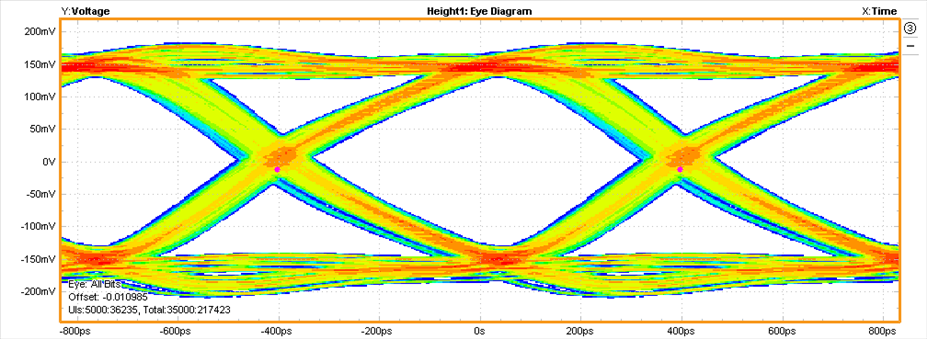
\includegraphics[width=0.8\linewidth]{sp-tpcelec-128Gbpseyesim.png}
\end{dunefigure}


%%%%%%%%%
\subsubsection{Alternative \dword{asic} Solutions}
\label{sec:fdsp-tpcelec-design-asic-alternatives}

%%%%%%%%%
\subsubsubsection{Commercial Off-the-shelf \dword{adc} Option}
\label{sec:fdsp-tpcelec-design-femb-alt-cots}

The \dword{sbnd} collaboration has been exploring the \dword{cots} \dword{adc} option 
for the \dword{tpc} readout electronics development since spring
2017~\cite{Chen:2018zic}. After a market survey, a few candidate \dwords{adc} 
using the \dword{sar} architecture were identified that would continue
to operate correctly when immersed in \lntwo. Starting in
July 2017, a lifetime study plan was developed to evaluate a \dword{cots} 
\dword{adc} option in two different phases: exploratory and validation. The 
lifetime study focused on the Analog Devices AD7274\footnote{AnalogDevices,
  AD7274\texttrademark{}, \url{https://www.analog.com/en/products/ad7274.html}.},
implemented in \dword{tsmc} \SI{350}{nm} \dword{cmos} technology, and has
demonstrated better performance in cryogenic operation compared to other candidates.

During the exploratory phase, fresh samples of the \dword{cots} \dword{adc} 
AD7274 were stressed with higher than nominal operation voltage, e.g.~\SI{5}{V},
while power consumption (drawn current) was monitored continuously. 
Periodically, the sample would be operated at nominal voltage (V$_{DD}$ = \SI{2.5}{V} 
and V$_{REF}$ = \SI{1.8}{V}) for a performance characterization test, where 
both the \dword{dnl} and \dword{inl} were monitored and analyzed in addition 
to the current. Stress test results were used to extrapolate the 
lifetime of the \dword{cots} \dword{adc}. The relation between the lifetime 
of \dword{cmos} transistors $\tau$ and the drain-source voltage $V_{ds}$, 
$\log\tau\propto1/V_{ds}$, is based on the creation of interface states by hot 
electrons and has been studies in the past extensively~\cite{Li:CELAr}.
The linear extrapolation of $\log\tau\propto1/V_{ds}$ is also used in industry (e.g. IBM) 
in accelerated stress testing. It was determined that a current drop 
of \num{1}\% on the V$_{DD}$ would be used as the degradation criterion for the lifetime 
study. In the validation phase, more devices were tested following the developed 
criteria to collect more data to validate what was learned in the exploratory phase.

The lifetime projection of the AD7274 \dword{adc} from the stress 
test with V$_{DD} >$ \SI{5}{V} is shown in Figure~\ref{fig:cotsadc-lifetime}. 
With the AD7274 operating at \SI{2.5}{V}, which is lower than the nominal 
\SI{3.6}{V} for the \SI{350}{nm} \dword{cmos} technology, the projected lifetime 
is more than than \num{1e6} years.

\begin{dunefigure}
[Lifetime projection of the COTS ADC]
{fig:cotsadc-lifetime}
{Lifetime projection of the \dword{cots} \dword{adc} AD7274 from the stress test 
with V$_{DD} >$ \SI{5}{V}. The current drop of 1\% on the V$_{DD}$ is used as 
the degradation criterion. With nominal operation voltage of \SI{3.6}{V} for the 
\SI{350}{nm} \dword{cmos} technology, the lifetime is projected to be more 
than 100 years. For \dword{sbnd} and \dword{dune} \dword{fd}, the AD7274 will be
operated at \SI{2.5}{V} to add an additional margin; the expected lifetime is more 
than \num{1e6} years.}
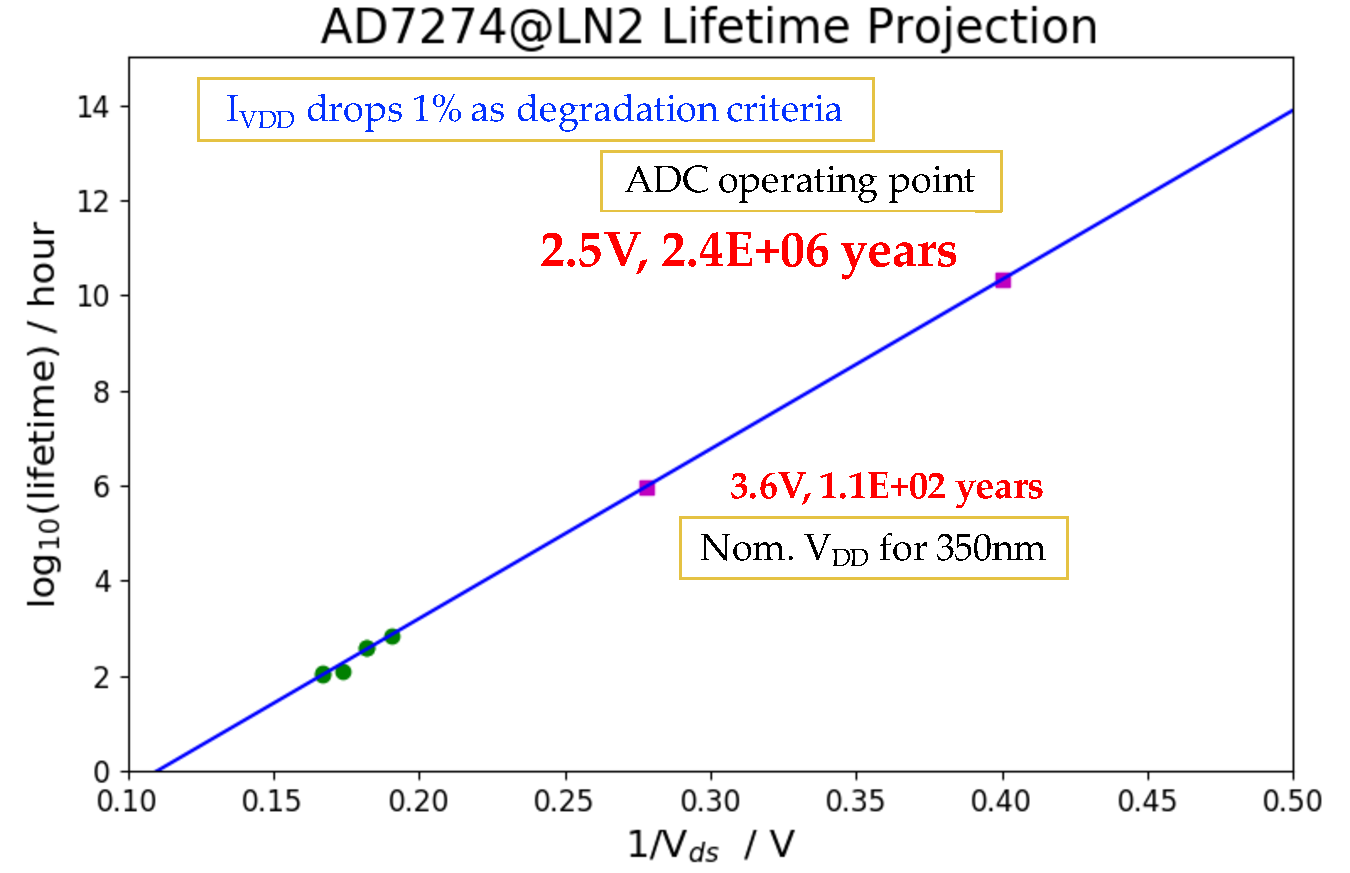
\includegraphics[width=0.8\linewidth]{sp-tpcelec-cotsadc-lifetime.pdf}
\end{dunefigure}

Based on the lifetime study of AD7274, a \dword{femb} with the \dword{cots} 
\dword{adc} was developed and characterized for the \dword{sbnd} experiment. The 
integration test was carried out with 40\% \dword{apa} at \dword{bnl} and 
showed satisfactory noise performance as seen in Figure~\ref{fig:cotsadc-fembenc}.
The noise measurements obtained with the  40\% \dword{apa} at \dword{bnl} indicate
that the AD7274 gives a negligible contribution to the overall system noise, as
expected given that the \dword{adc} has a \dword{enob}
of 11.4 bits. The \dword{cots} \dword{adc} AD7274 serves as a backup solution for the 
\dword{dune} \dword{fd} \dword{tpc} readout electronics system. The current 
plan is to evaluate this \dword{adc} in the small \dword{tpc} installed in
\dword{iceberg} at \dword{fermilab}. Ten \dwords{femb} with the \dword{cots} 
\dword{adc} are being produced and will be used to instrument the \dword{iceberg} 
\dword{tpc} for system integration tests in spring 2019. The main drawback of
the AD7274 \dword{adc} is that it is a single channel chip, complicating the 
assembly of the \dwords{femb}.

\begin{dunefigure}
[Noise measurement of FEMBs with COTS ADC]
{fig:cotsadc-fembenc}
{The noise measurement of \dwords{femb} with \dword{cots} \dwords{adc} 
mounted on the \num{40}\% APA at \dword{bnl}. A picture of the 
\dword{femb} is shown in the top left corner. The induction plane 
(\SI{4}{m} wire) has a noise level of $\sim\SI{400}{e^-}$ with \SI{1}{$\mu$s} 
peaking time, while the collection plane (\SI{2.8}{m} wire) has a noise level
of $\sim\SI{330}{e^-}$ with \SI{1}{$\mu$s} peaking time.}
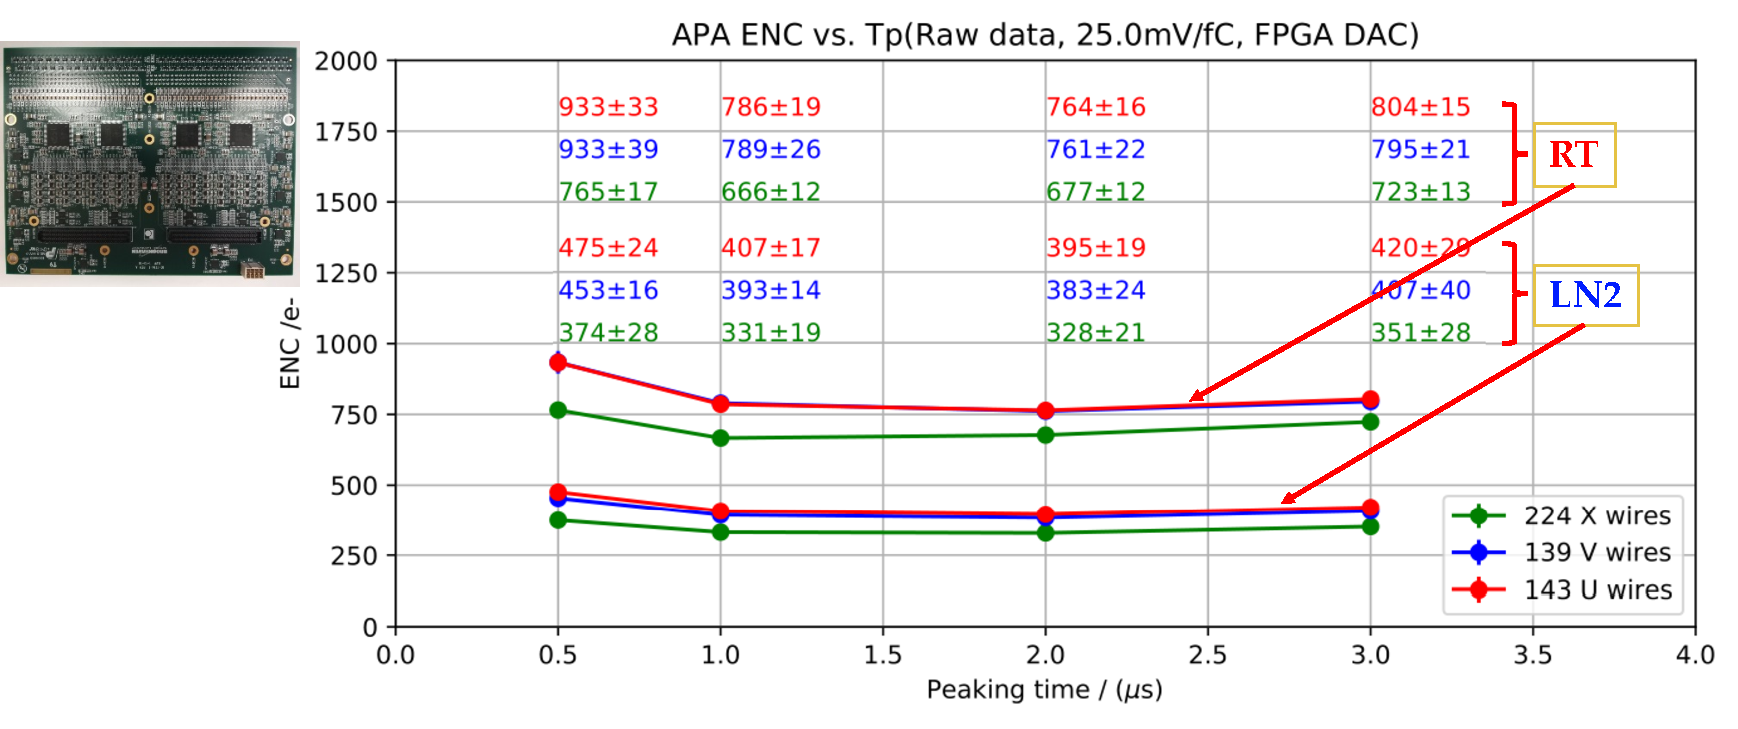
\includegraphics[width=0.99\linewidth]{sp-tpcelec-cotsadc-fembenc.pdf}
\end{dunefigure}

%%%%%%%%%
\subsubsubsection{CRYO Option}
\label{sec:fdsp-tpcelec-design-femb-alt-cryo}


The \dword{slac} \dword{cryo} \dword{asic} differs from the baseline three-chip 
design by combining the functions of an analog preamplifier, \dword{adc}, and 
data serialization along with transmission for \num{64} wire channels into a single 
chip. It is based on a design developed for the \dword{nexo} experiment~\cite{nEXO} 
and differs from it only in the design of the preamplifier, which is modified for 
the higher capacitance of the \dword{dune} \dword{spmod} wires compared to the short
strips of \dword{nexo}. The \dwords{femb} constructed using this chip would use only 
two \dwords{asic}, compared to the \num{18} (eight \dword{larasic}s, eight \dword{coldadc}s and 
two \dword{coldata}s) needed in the baseline design. This drastic reduction in 
part count may significantly improve \dword{femb} reliability, reduce power 
(\SI{40}{mW} per channel), and reduce costs related to production and testing.

Figure~\ref{fig:cryo-schematic} shows the overall architecture of the 
\dword{cryo} \dword{asic}, which is implemented in \SI{130}{nm} \dword{cmos}. 
It comprises two identical 32-channel blocks (banks) and a common section
providing biasing voltages and currents plus the controls signals, the clocks 
generation and the configuration of the registers.

\begin{dunefigure}
[Overall architecture of the CRYO ASIC]
{fig:cryo-schematic}
{Overall architecture of the \dword{cryo} \dword{asic}.}
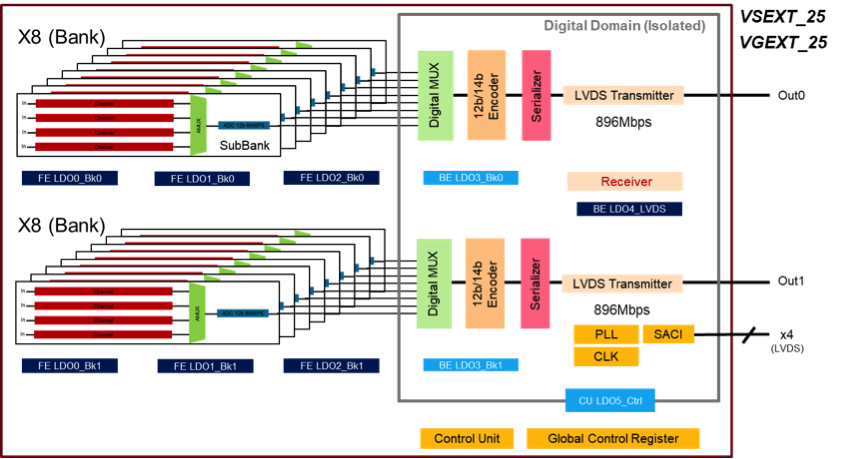
\includegraphics[width=0.9\textwidth]{sp-tpcelec-cryo-schematic.png}
\end{dunefigure}

The current signal from each wire is amplified using a preamplifier with pole 
zero cancellation~\cite{DeGeronimo:2011zz} and an anti-alias fifth-order 
Bessel filter (Fig.\ref{fig:cryo-FE}). Provisions are also made for injection 
of test pulses. Gain and peaking time are adjustable to values similar to 
those of the baseline design. 
The four programmable gain settings 6X, 3X, 1.5X, and 1X correspond to full scale signals of 
$\SI{3.2e5}{e^{-}}$, $\SI{6.4e5}{e^{-}}$, $\SI{1.28e6}{e^{-}}$, and $\SI{1.92e6}{e^{-}}$. A 
filter with a Bessel shape has been chosen because of its flat group delay characteristic 
which minimize waveform distortion as well as providing noise shaping performance similar 
to more classic semi-Gaussian shaper implementations. The four programmable peaking times 
of the filter range from $\SI{0.6}{{\mu}s}$, $\SI{1.2}{{\mu}s}$, $\SI{2.4}{{\mu}s}$, 
and $\SI{3.6}{{\mu}s}$, corresponding to filter bandwidths equivalent to the ones used in 
the baseline solution. Similarly to the baseline design the channel provides the possibility 
to set the baseline for operation with either the collection or the induction wires. 
Baseline level can be set and trimmed independently in each single channel. Channel 
outputs can be connected one-at-a-time to an analog monitor to probe the analog signal.

\begin{dunefigure}
[CRYO FE section architecture and typical front-end response]
{fig:cryo-FE}
{\dword{cryo} front-end section architecture (left); typical response of the \dword{cryo} front-end (right).}
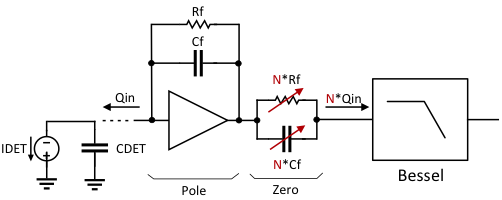
\includegraphics[width=.54\textwidth]{sp-tpcelec-cryo-feschematic.png}
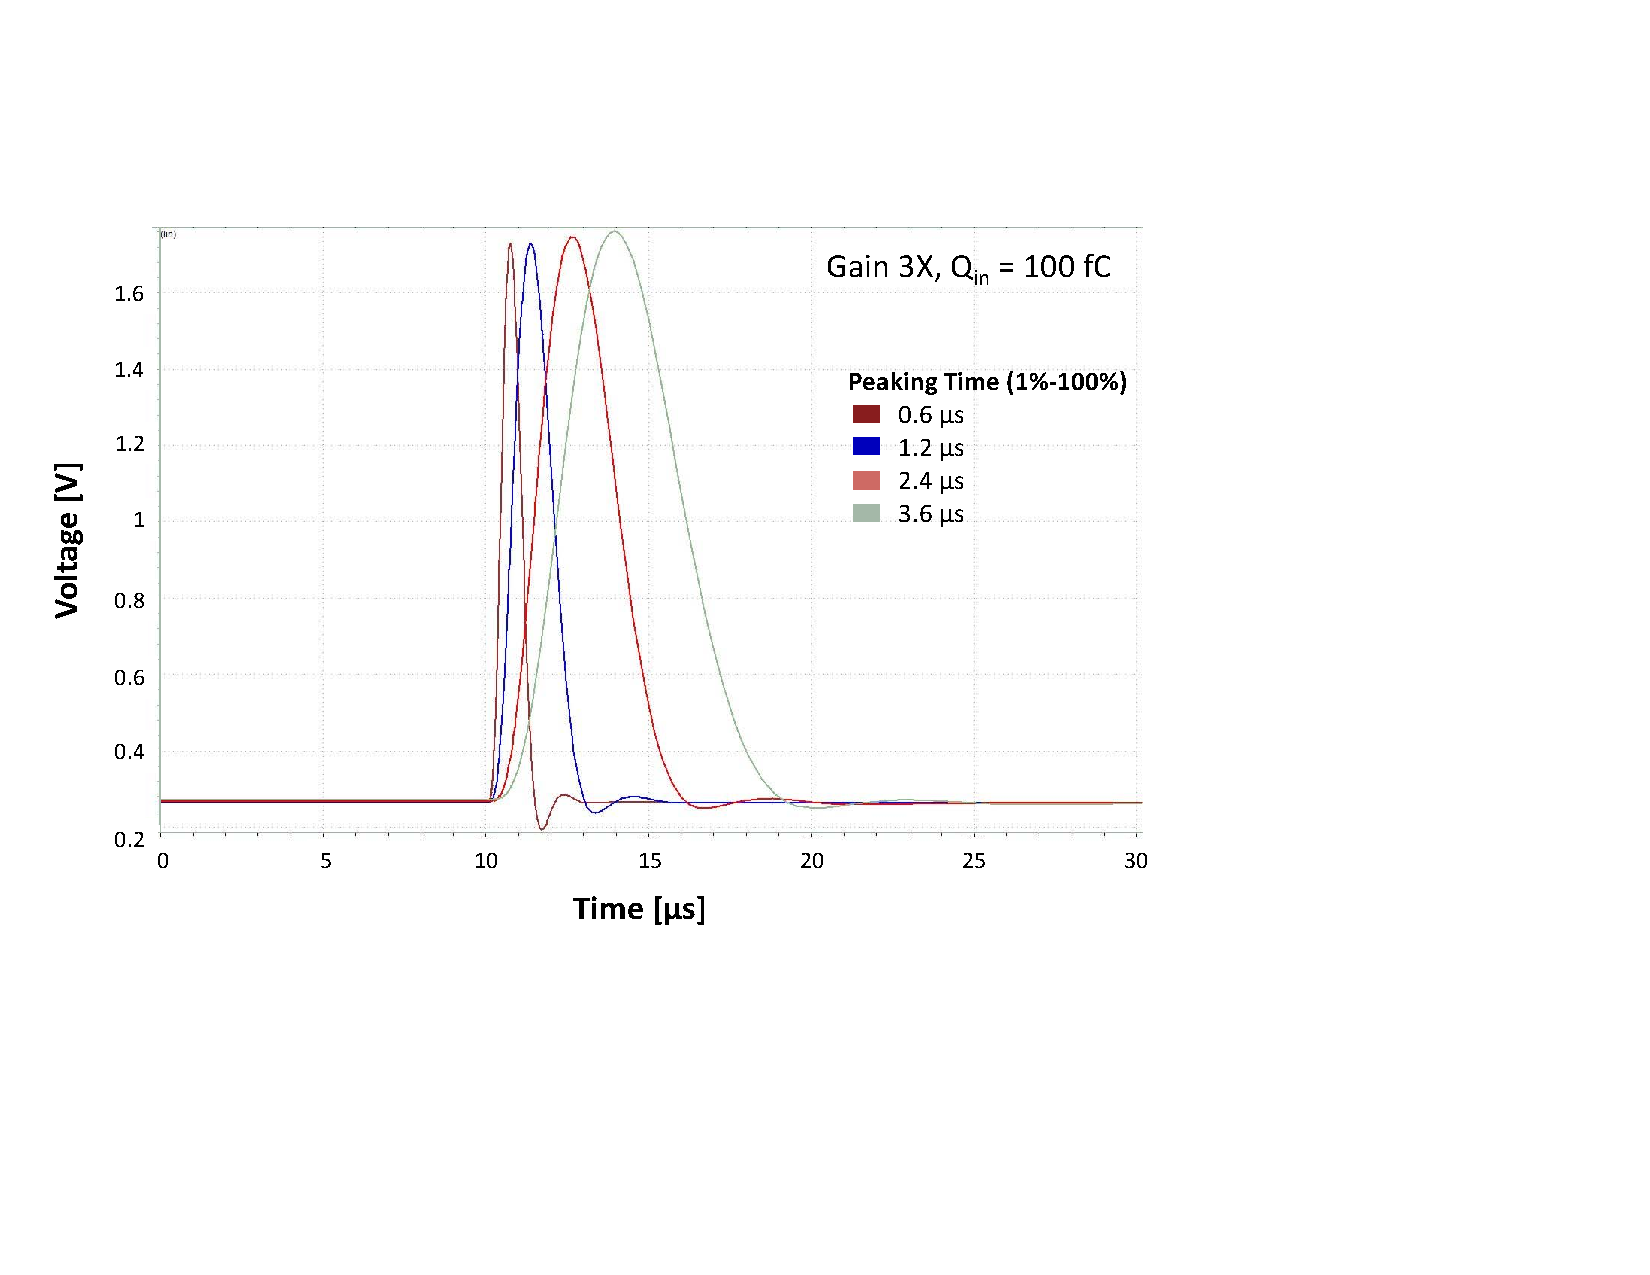
\includegraphics[width=.45\textwidth,trim={0 5.5cm 6.5cm 3cm},clip]{sp-tpcelec-cryo-filter.pdf}
\end{dunefigure}

Four input channels are multiplexed onto a single fully differential 12 bit \SI{8}{MSPS} 
\dword{adc}. Signals from the four channels are concurrently sampled onto a Sample and Hold 
stage. An \dword{adc} driver after the multiplexer performs the single-ended to differential 
conversion. The \dword{adc} has a pure \dword{sar} architecture (Figure~\ref{fig:cryo-ADC}) with a split 
cap \dword{dac} based on V$_{cm}$ switching~\cite{5482529}, and has the option to be 
calibrated for offset compensation.

\begin{dunefigure}
[CRYO ADC architecture]
{fig:cryo-ADC}
{\dword{cryo} \dword{adc} architecture.}
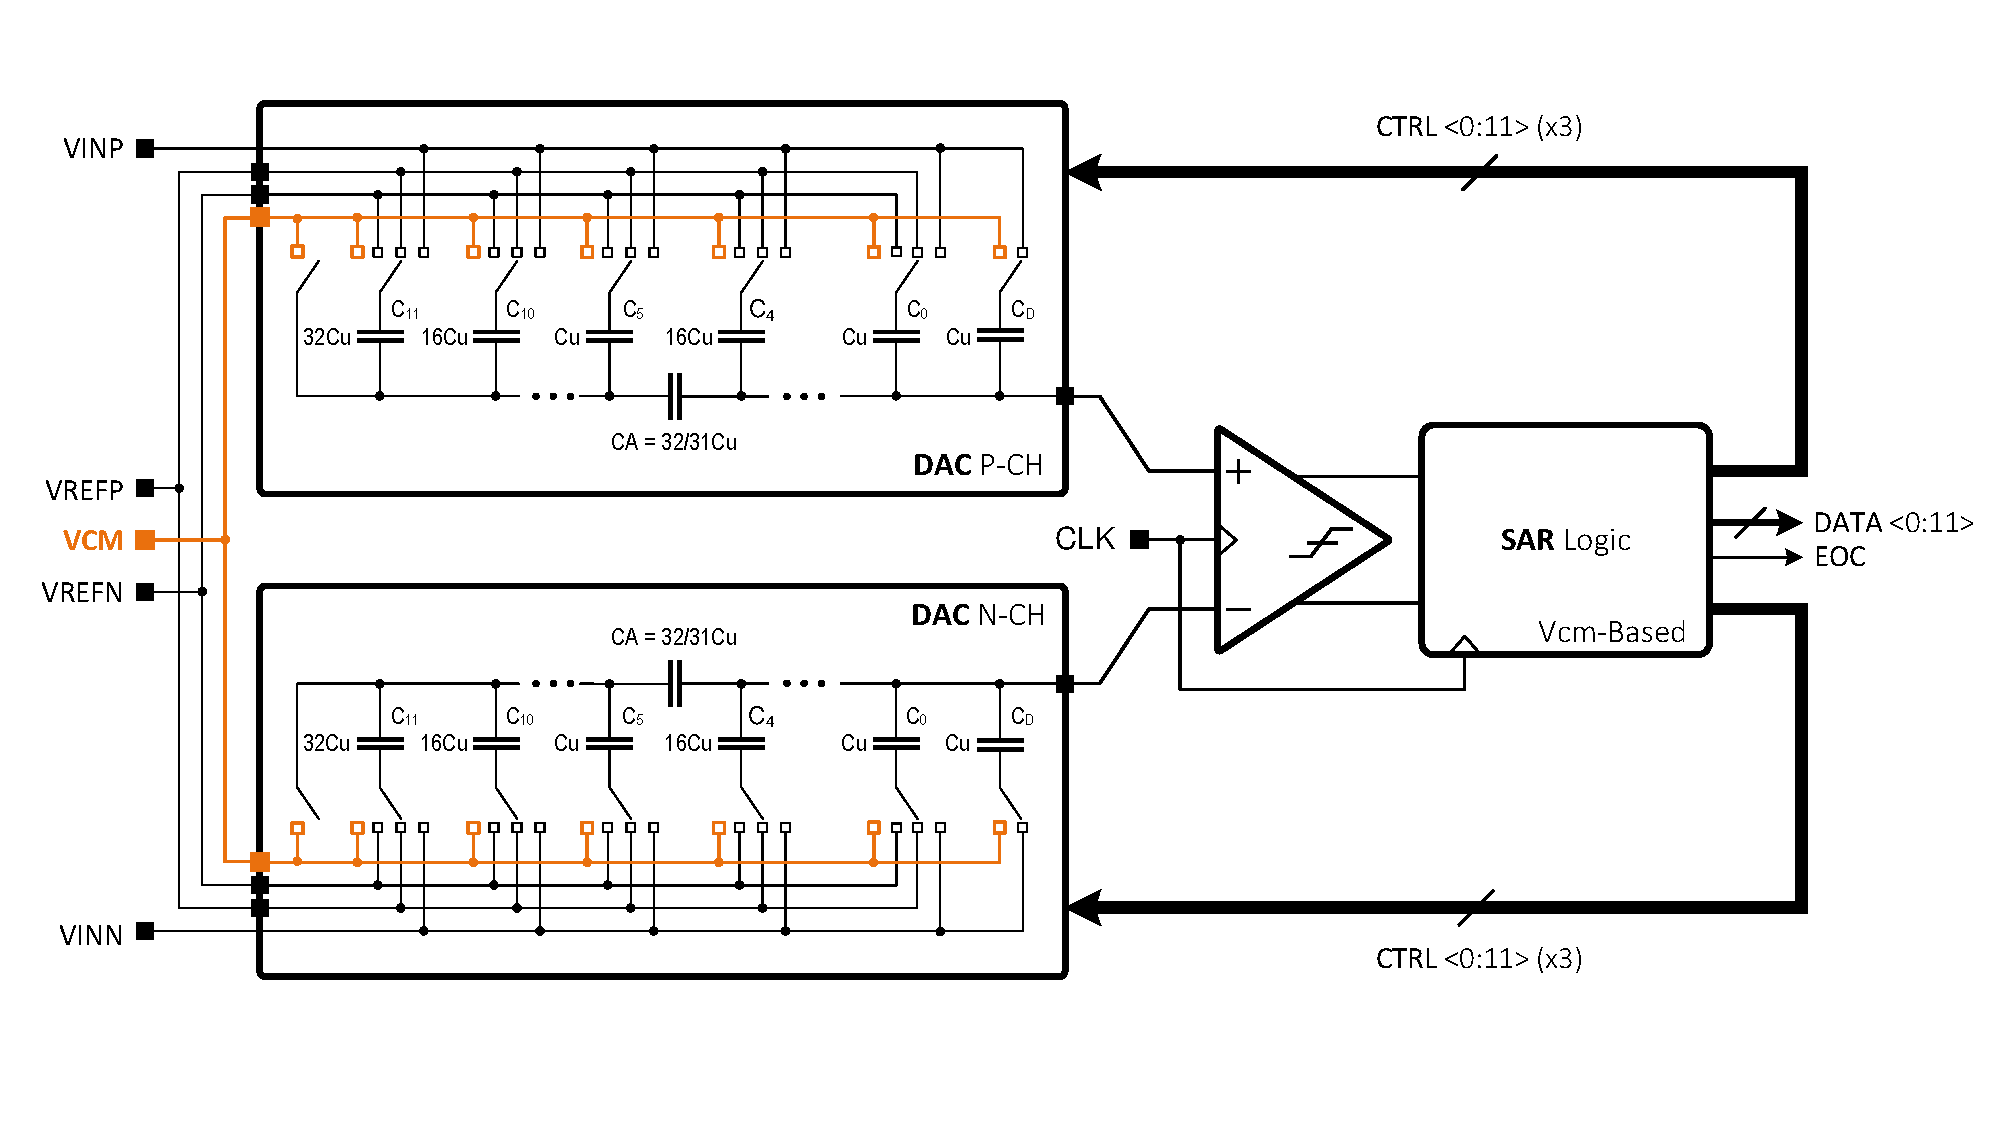
\includegraphics[width=.9\textwidth]{sp-tpcelec-cryo-adcschematic.pdf}
\end{dunefigure}

External signals can be routed to the input of each single \dword{adc} allowing standalone characterization.

The data serialization and transmission block uses a custom 12b/14b encoder, so 32 channels 
of 12-bit, \SI{2}{MSPS} data can be transmitted with a digital bandwidth of only \SI{896}{Mbps}, 
which is significantly lower than the required bandwidth of the baseline, which is \SI{1.28}{Gbps}.

One key concern with mixed signal \dwords{asic} is the possibility of interference from the 
digital side causing noise on the very sensitive preamplifier. To avoid this interference, 
the \dword{cryo} design uses well established techniques for isolating the substrate;
these are described in the literature~\cite{yeh} and have been successfully used in previous 
\dwords{asic}. Furthermore power domains of the various sections of the \dwords{asic} are 
isolated using multiple internal \dwords{ldo}.

For reliability purposes the analog section of the \dword{asic} using thick oxide devices 
is biased at 2V (20\% less than nominal voltage) and does not use minimum length devices.
The digital section of the \dword{asic} uses instead core devices biased at 1V (again 20\% 
less than nominal voltage).

The infrastructure requirements for a \dword{cryo} \dword{asic}-based system are similar 
to those of the baseline option. However, in most cases, somewhat fewer resources are 
needed; for instance:
\begin{itemize}
\item A single voltage is needed for the power supply. This is used to generate the two 
supply voltages using internal voltage regulators.
\item The warm interface is different. \dword{cryo} operates synchronously
with a \SI{56}{MHz} clock, does not require a fast command, and uses the 
SACI~\cite{SACI} protocol for configuration rather than \dword{i2c}.
\end{itemize}

Simulation-based studies have been performed; at $\SI{1.2}{{\mu}s}$ peaking time and an 
input capacitance of \SI{220}{pF} (similar to that expected in the \dword{spmod}), the noise 
level is approximately $\SI{500}{e^{-}}$, similar to that expected with the baseline 
\dword{larasic} design in \dword{lar} with the same input capacitance.

The first iteration of the \dword{cryo} \dword{asic} design (see Figure~\ref{fig:cryo-photos}) 
was submitted to MOSIS for fabrication in November 2018. The first prototypes were 
delivered at the end of January 2019.

\begin{dunefigure}
[Photos of CRYO ASIC prototype]
{fig:cryo-photos}
{Photo of the prototype cold board (left); zoomed-in photo of \dword{cryo} \dwords{asic} (right).}
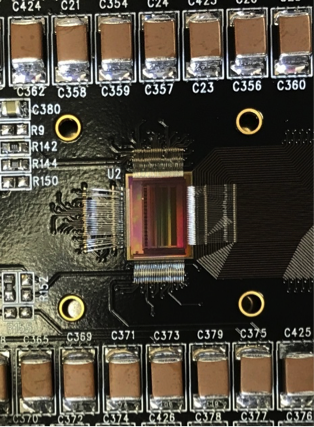
\includegraphics[width=.3\textwidth]{sp-tpcelec-cryo-coldboard.png}
\hspace{1cm}
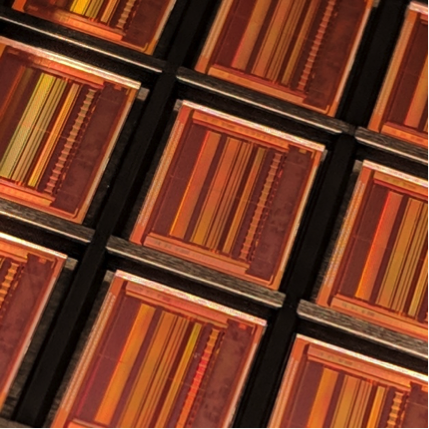
\includegraphics[width=.4075\textwidth]{sp-tpcelec-cryo-cryophoto.png}
\end{dunefigure}

The prototypes are under test in an existing test stand at \dword{slac} using the \dword{cts}
described in Section~\ref{sec:fdsp-tpcelec-qa-initial}. Subsequent system tests are planned 
using the facilities described in Section~\ref{sec:fdsp-tpcelec-qa-facilities}.

The first prototype of the \dword{asic} is functional at both room temperature and \lntwo 
temperature. In particular all the key blocks have been verified. Configuration of all the 
64 channel registers (13 bits each) and the 17 (16-bit) global registers has been 
verified. Optimization of the register values at room temperature and cold is 
ongoing. Initialization procedures for the \dword{asic} power up have been established. 
Operation of the on-chip \dwords{ldo} has been verified and expected supply levels are 
stable across temperature. Injected pulses on the front-end channels are visible on 
the analog monitor (Figure~\ref{fig:cryo-FEresponse}) as well as they are digitized 
with the internal \dwords{adc}.

\begin{dunefigure}
[CRYO ASIC FE response at liquid nitrogen temperature]
{fig:cryo-FEresponse}
{\dword{cryo} \dword{asic} front-end response at liquid nitrogen temperature, presented at the analog monitor and acquired with an external \SI{50}{MSPS} \dword{adc}.}
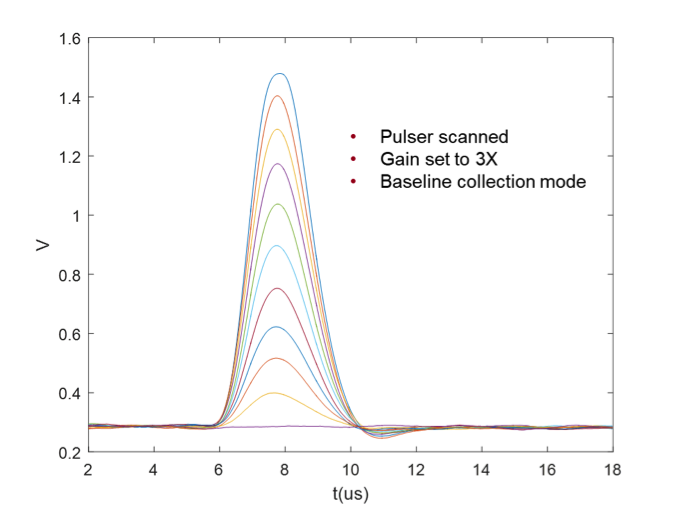
\includegraphics[width=.65\textwidth]{sp-tpcelec-cryo-pulses.png}
\end{dunefigure}

Encoded data are transmitted and correctly decoded in the external \dword{fpga}. 
Figure~\ref{fig:cryo-analogmon} shows an example of a pulse injected in a channel 
visible on both the analog monitor as well as in the data acquired by the \dword{asic}. 
Data are acquired at \lntwo temperature at the nominal $\sim$\SI{2}{MSPS} rate.

\begin{dunefigure}
[Example of a pulse injected in a CRYO ASIC channel]
{fig:cryo-analogmon}
{Example of a pulse injected in a \dword{cryo} \dword{asic} channel, visible on both the analog monitor and in the output data.}
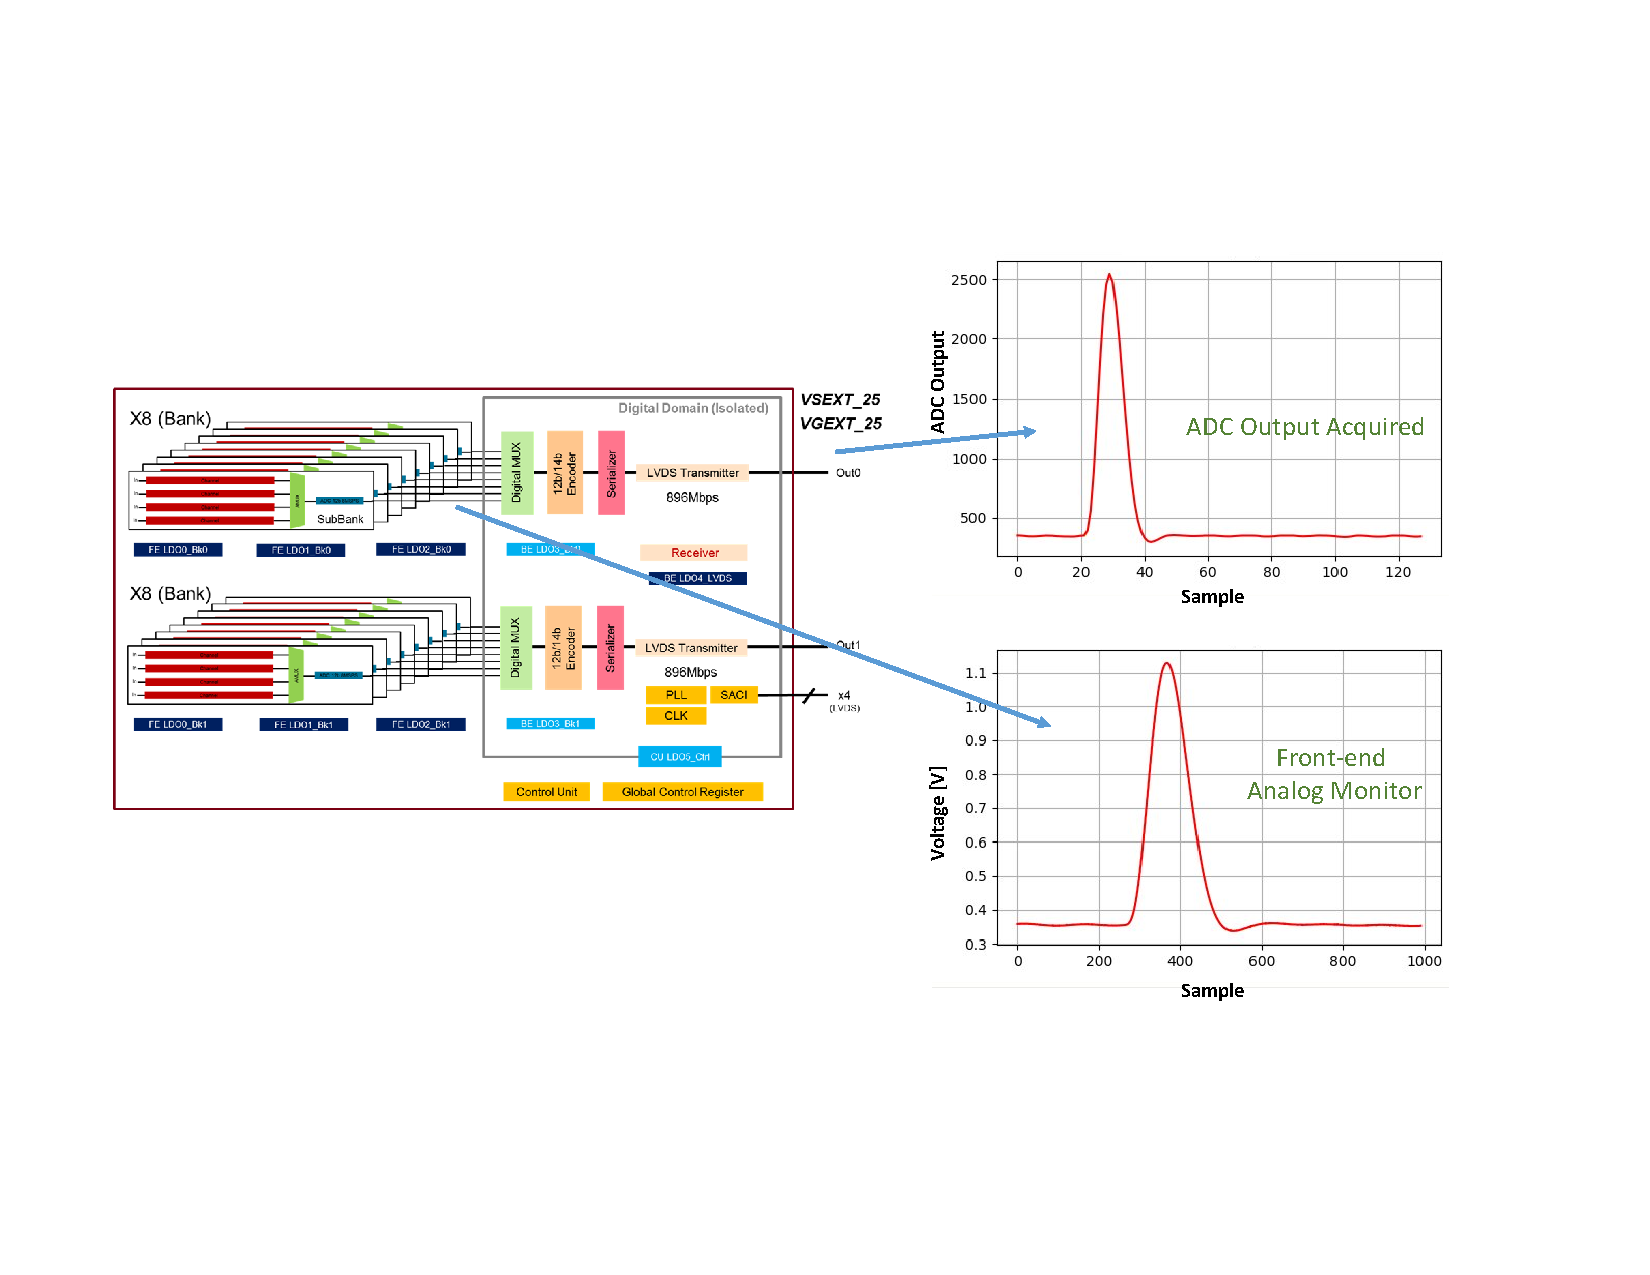
\includegraphics[width=.99\textwidth,trim={1cm 4cm 3cm 3cm},clip]{sp-tpcelec-cryo-analogmonitor.pdf}
\end{dunefigure}

From the functional point of view, a single unexpected behavior has been identified 
in the digital multiplexer that is used at the input of the encoders. The latches
at the input of the multiplexer show poor driving capability resulting in a presence
of a ghost from a previously multiplexed channel. The effect is not present on the 
first 12 channels of each block which show expected behavior. The effect has been
understood replicated in simulation and a trivial fix has been implemented for 
the next version of the \dword{asic}.

Initial results on the performance of the \dword{adc} block of \dword{cryo} have
been obtained by directly injecting a linear ramp (generated by an external
\num{20}-bit \dword{dac}) into the \dword{adc}. The distributions of the \dword{dnl}
and \dword{inl} obtained from these measurements are shown in Figure~\ref{fig:cryo-dnlinl}.
The maximum deviations of the \dword{dnl} and \dword{inl} from the reference
signal are \num{0.74} and \num{1.27} \dword{adc} counts, respectively, within
a usable dynamic range of $\sim\num{3000}$ \dword{adc} counts. From these
distributions the values for the \dword{sndr} of \SI{65.75}{dB} and for
the \dword{enob} of \SI{10.63}{bits} are estimated. These results indicate
that from a static point of view the \dword{adc} block of \dword{cryo}
meets the required performance for the \dword{dune} \dword{tpc} readout.
Further work is ongoing to characterize the dynamic response of the
\dword{adc} and to determine the overall linearity and noise performance
of the entire readout chain including the \dword{fe} amplifier.

\begin{dunefigure}
[Differential and integral non-linearities for the CRYO ADC]
{fig:cryo-dnlinl}
{Distribution of the \dword{dnl} (left) and \dword{inl} (right) for the
\dword{adc} block of \dword{cryo}.}
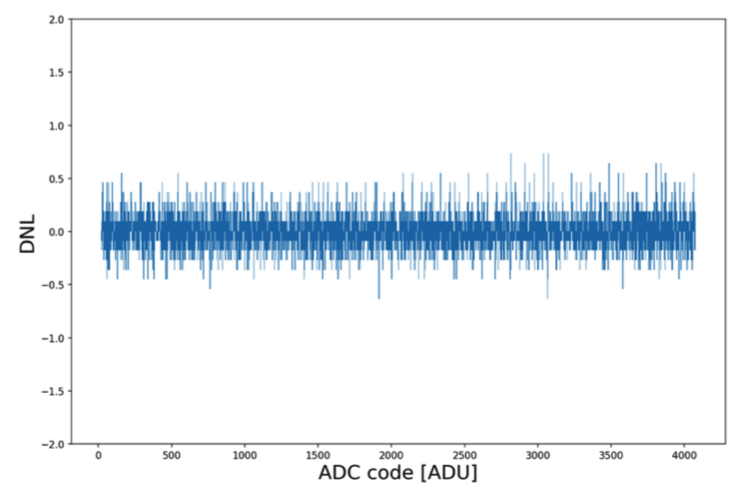
\includegraphics[width=.45\textwidth]{sp-tpcelec-cryo-dnl.png}
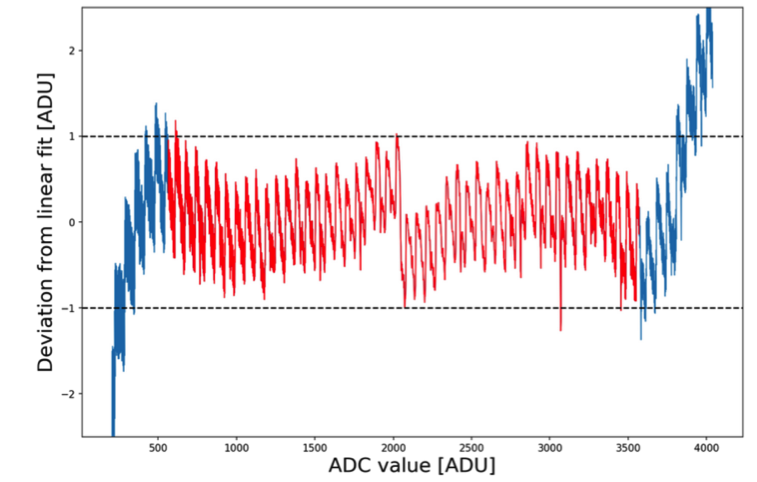
\includegraphics[width=.45\textwidth]{sp-tpcelec-cryo-inl.png}
\end{dunefigure}

%%%%%%%%%%%%%%%%%%
\subsubsection{Procedure and Timeline for \dword{asic} Selection}
\label{sec:fdsp-tpcelec-design-femb-selection}

We are currently pursuing two different \dword{asic} designs and 
planning on qualifying the \dword{cots} \dword{adc} solution that 
will be used for the \dword{sbnd} experiment.
We plan to continue developing both the three-\dword{asic} 
solution and the \dword{cryo} \dword{asic} for at least a second 
iteration before deciding which \dword{asic} solution to 
implement in the \dword{dune} \dword{spmod}. This plan requires
that multiple flavors of the \dword{femb} are also designed 
and tested. The \dwords{femb} populated with the first set of prototypes of 
the two kinds of \dwords{asic} will be available in late summer 2019 
and are expected to have a performance at least similar to that 
of the boards used for \dword{pdsp}. We plan to review the results 
of the system tests and of the component lifetimes discussed 
in Section~\ref{sec:fdsp-tpcelec-qa} in fall 2019. 
In that review, we will also decide whether to change anything on 
the list of specifications for the \dwords{asic} and to further develop
the two custom \dword{asic} solutions, including fixing any 
issues found during the tests of the first version of the \dwords{asic}. 
We expect that the subsequent iteration
of the design, fabrication, and testing of the \dwords{asic} and
\dwords{femb} will take an additional twelve months. At the end 
of this process, when results from standalone tests of the
\dwords{asic} and system tests of the \dwords{femb} are
available, we should be in position to decide which \dword{asic}
solution to adopt. We are assuming that the second iteration of
the \dwords{asic} design will meet all the \dword{dune} requirements.
The schedule for the construction of the \dword{dune} \dword{spmod}
currently has between eight and fourteen months of float for the
\dwords{asic} and \dwords{femb}, which would allow for a third 
design iteration, in case that would be needed, as discussed
in Section~\ref{sec:fdsp-tpcelec-management-planning}. This does
not apply for the second run of \dword{pdsp} (discussed
later in Section~\ref{sec:fdsp-tpcelec-qa-facilities-pdune}).
Ideally for the second run of \dword{pdsp} the \dwords{asic}
from the engineering run would be used, but this is not compatible
with the currently planned date for the installation of the \dwords{femb}
on the \dwords{apa}. In order to meet the current goal for the starting
date of the second run of \dword{pdsp}, \dwords{asic} from the
second round of prototyping would have to be used. In case a
third round of prototypes is necessary, the second run of 
\dword{pdsp} would have to be delayed by one year.

The selection of the \dword{asic}(s) to be used for the
construction of the \dword{sp} \dword{detmodule} will be
based on performance, reliability, power density
criteria, as well as consideration of the costs and
resources required during the construction and testing
of the \dwords{femb}. We have not yet decided what weight 
to assign to these criteria. Reliability would in principle favor
the single-\dword{asic} solution that requires 
\dwords{femb} with fewer connections, while power 
density considerations could be less favorable to \dword{cryo}.
We plan to charge a committee to draft a series of recommendations 
on the \dword{asic} selection in fall 2019, at least one year
ahead of the expected decision date. These recommendations could 
also inform the second cycle of design for
\dwords{asic} and \dwords{femb}. Once the second cycle of design
and testing is complete, these recommendations will be used by the
committee charged with the final design review to suggest a
preferred option for the \dword{asic} solution.
The committee's recommendation 
will then be passed to the \dword{dune} \dword{exb}, 
which is tasked with the final \dword{asic} decision.

%%%%%%%%%%%%%%%%%%%%%%%%%%%%%%%%%%%
\subsection{Infrastructure Inside the Cryostat}
\label{sec:fdsp-tpcelec-design-infrastructure}

Each \dword{femb} is enclosed in a mechanical \dword{ce} box 
to provide support, cable strain relief, and control of bubbles of gaseous
argon generated by heat from an \dword{femb} attached to the lower \dword{apa},
which could, in principle, lead to discharge of the \dword{hv} system. The
\dword{ce} box, illustrated in Figure~\ref{fig:ce-box}, is designed to make the 
electrical connection between the \dword{femb} and the \dword{apa} 
frame, as discussed %defined 
in Section~\ref{sec:fdsp-tpcelec-design-grounding}.
Mounting hardware inside the \dword{ce} box connects the ground plane 
of the \dword{femb} to the box casing. If argon bubbles %are formed 
form inside
the \dword{ce} box, they must get %these should be 
channeled through the two side
\dword{apa} frames, from where they would reach the top of the cryostat.
As already discussed in Section~\ref{sec:fdsp-tpcelec-overview-requirements},
a test setup is being prepared at \dword{bnl} to measure the
maximum power that can be dissipated in \dword{lar} at a
depth equivalent to those of the \dwords{femb} installed on
the bottom \dword{apa}. Together with measurements of the
power consumption by new \dwords{asic}, this will inform
the need for further design of a system to collect any
argon bubbles and channel them through the \dword{apa} frames.

\begin{dunefigure}
[Prototype CE box used in ProtoDUNE-SP]
{fig:ce-box}
{Prototype \dword{ce} box used in \dword{pdsp}.}
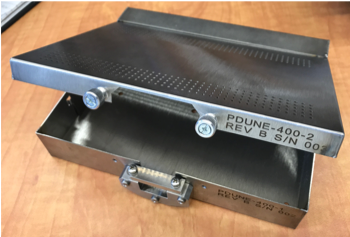
\includegraphics[width=0.45\linewidth]{sp-tpcelec-CEbox.png}
\end{dunefigure}

The \dword{ce} box casing is electrically connected to the 
\dword{apa} frame via the metal mounting hardware, called the 
Omega bracket (not shown in Figure~\ref{fig:ce-box}). The 
input amplifier circuits  are connected to the \dword{cr} board  
and terminate to ground at the \dword{apa} frame, as 
shown in Figure~\ref{fig:CR-board}.  As a backup, the casing is 
also connected to the \dword{apa} frame via a wire.

In addition to the \dword{ce} box and mounting hardware, cable trays 
for support and routing the cold cables will be installed in the 
cryostat. One set of cable trays, shown in Figure~\ref{fig:trays} 
(left column), will be attached to the upper \dword{apa} itself 
to hold the \dword{ce} and \dword{pd} cables. A different cable 
tray design, also shown in Figure~\ref{fig:trays} (right column), 
will support the \dword{ce} cables underneath the 
lower hanging \dword{apa}. A final set of cable trays will be 
installed inside the cryostat after the \dword{apa}s are 
fixed in their final location to support the cables as they are 
routed to the \dword{ce} and \dword{pd} feedthroughs.

\begin{dunefigure}
[Views of various cable and CE \coldbox{}es supports]
{fig:trays}
{Side and end views of mechanical supports for the \dword{ce} 
boxes on the upper (left column) and lower (right column) 
\dword{apa}s. Shown are the \dword{apa} cable trays in green and pink, 
the \dword{ce} boxes in dark gray, and the Omega brackets and mounting 
hardware between the \dword{ce} boxes and \dword{apa} frame in light gray.  
The \dword{ce} cables are shown in blue; the \dword{pd} cables are not shown.}
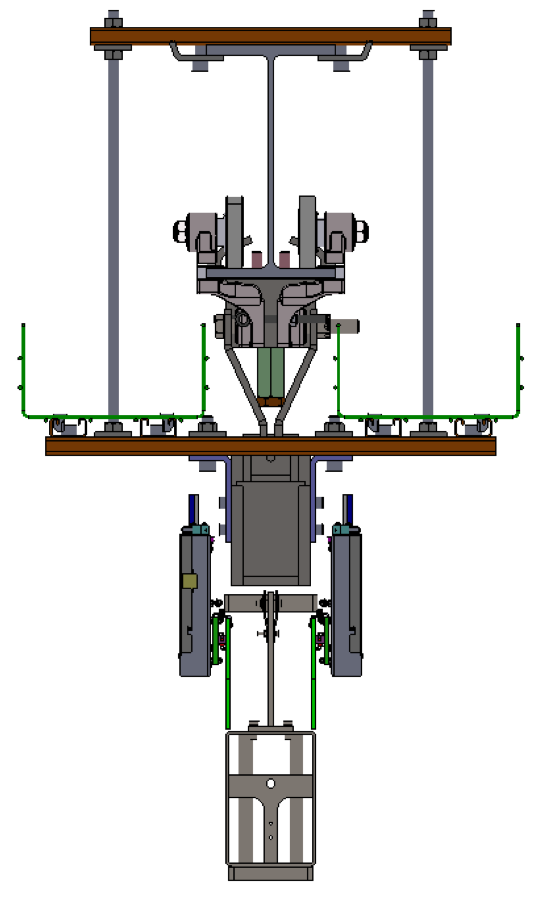
\includegraphics[width=0.38\linewidth]{sp-tpcelec-upper-tray2.png}
\hspace{5mm}
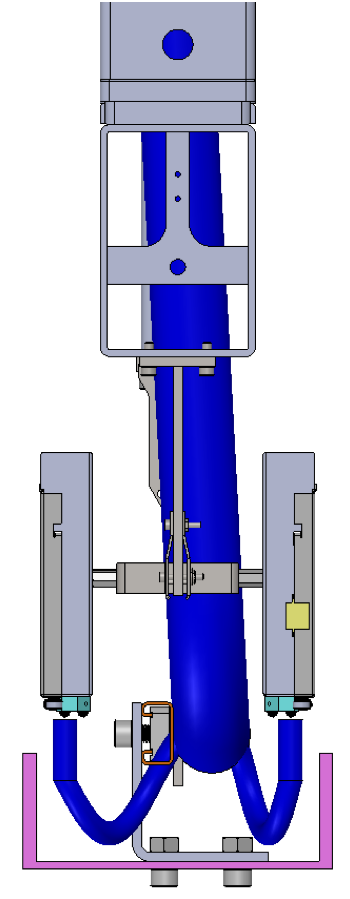
\includegraphics[width=0.25\linewidth]{sp-tpcelec-lower-tray2.png} \\
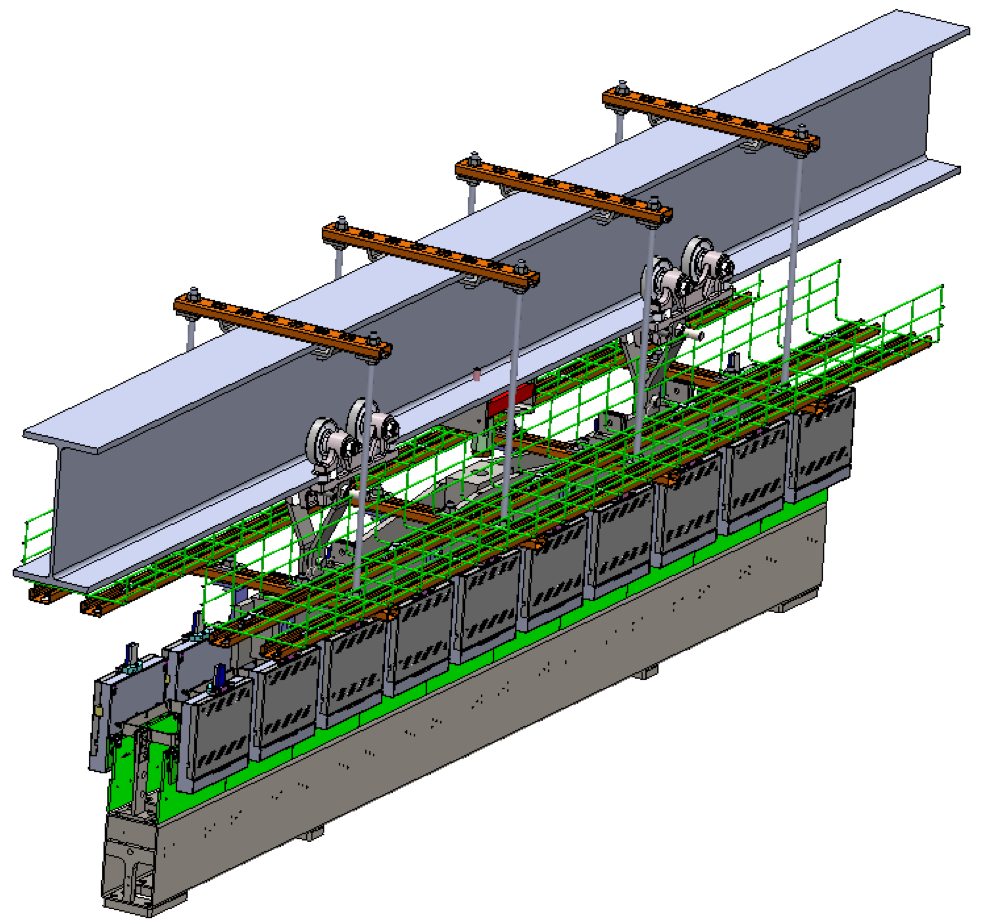
\includegraphics[width=0.32\linewidth]{sp-tpcelec-upper-tray1.png}
\hspace{5mm}
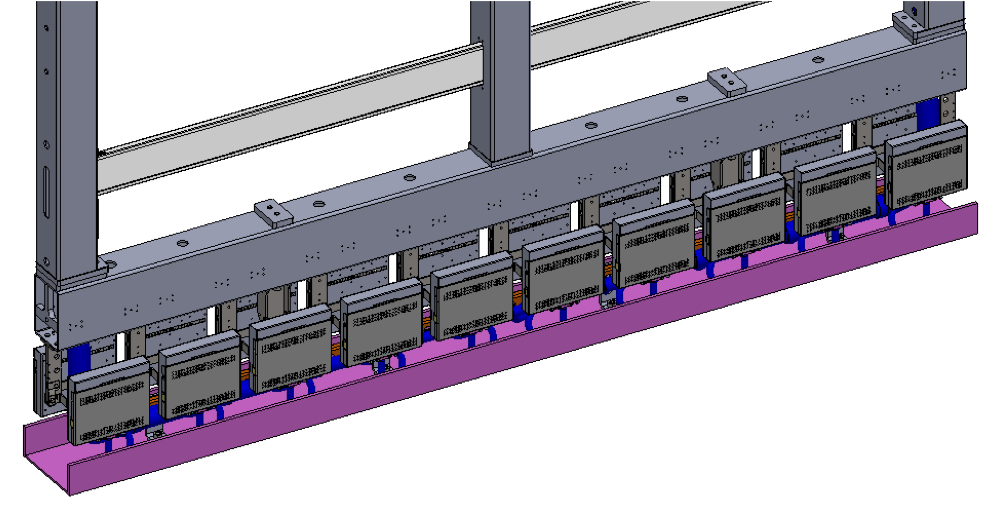
\includegraphics[width=0.4\linewidth]{sp-tpcelec-lower-tray1.png}
\end{dunefigure}


%%%%%%%%%%%%%%%%%%%%%%%%%%%%%%%%%%%
\subsection{Cold Cables and Cold Electronics Feedthroughs}
\label{sec:fdsp-tpcelec-design-ft}

All cold cables originating inside the cryostat connect to the outside 
warm electronics through \dword{pcb} \fdth{}s installed in the signal 
flanges that are located on the cryostat roof. The data rate from each
\dword{femb} with four cables is sufficiently low ($\sim\SI{1}{Gbps}$)
that \dword{lvds} signals can easily be driven over more than \SI{22}{m}
of twin-axial transmission line. Additional transmission lines
are available to distribute \dword{lvds} clock and control signals,
which are transmitted at a lower bit rate.
Optical fiber is used externally from the \dwords{wib} on the signal 
flange to the \dword{daq} (see Chapter~\ref{ch:sp-daq}) and slow 
control systems (see Chapter~\ref{ch:sp-cisc}).

\begin{dunefigure}
[TPC cold eletronics \fdth]
{fig:tpcelec-signal-ft}
{TPC \dword{ce} \fdth. The \dwords{wib} are seen edge-on in the left 
panel and in an oblique side-view in the right panel, which also shows 
the warm crate for an \dword{spmod} in a cutaway view.}
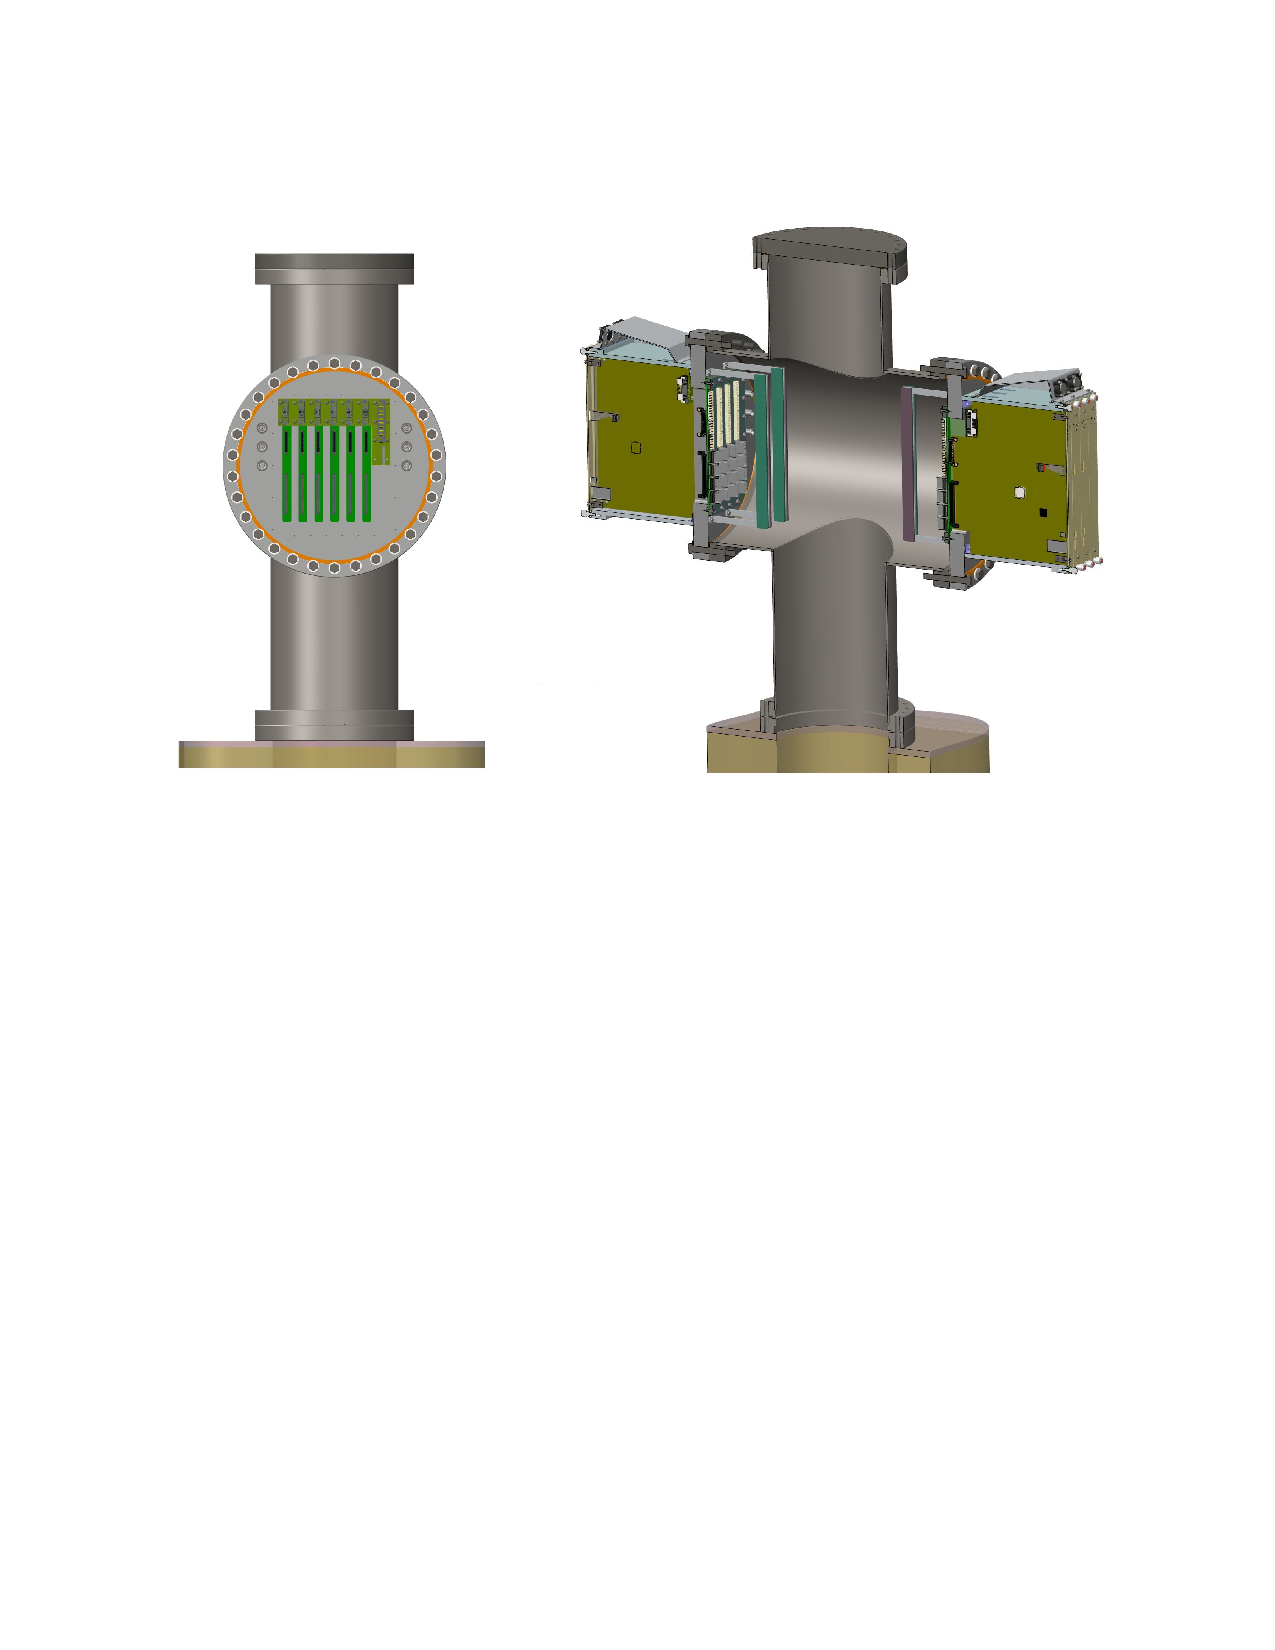
\includegraphics[width=0.9\linewidth]{sp-tpcelec-signal-FT.pdf}
\end{dunefigure}

The design of the signal flange includes a four-way cross spool 
piece, separate \dword{pcb} \fdth{}s for the \dword{ce} and 
\dword{pds} cables, and an attached crate for the \dword{tpc} 
warm electronics, as shown in Figure~\ref{fig:tpcelec-signal-ft}.
The wire bias voltage cables connect to standard \dword{shv} 
connectors machined directly into the \dword{ce} \fdth{}, ensuring 
no electrical connection between the wire bias voltages and other 
signals passing through the signal flange. Each \dword{ce} \fdth 
serves the bias, power, and digital I/O needs of one \dword{apa}.  

Data and control cable bundles send system clock and control signals 
from the signal flange to the \dword{femb} and stream the $\sim$\SI{1}{Gbps} 
high-speed data from the \dword{femb} to the signal flange. Each 
\dword{femb} connects to a signal flange via one data cable bundle, 
leading to \num{20} bundles between one \dword{apa} and one flange. 
For the baseline \dwords{asic} configuration \num{10} low-skew shielded 
twin-axial cables are required to transmit the following differential signals
between the \dword{wib} and the \dword{femb}:
\begin{itemize}
\item four \SI{1.28}{Gbps} data (two from each \dword{coldata});
\item two \SI{64}{MHz} clocks (one input to each \dword{coldata});
\item one fast command line (shared between the two \dword{coldata} \dwords{asic});
\item three \dword{i2c}-like control lines (clock, data-in, and data-out, also shared between the 
two \dword{coldata} \dwords{asic}).
\end{itemize}
As discussed later, this number of connections is compatible with routing
the cables bringing the power and transmitting the data and controls for
the lower \dword{apa} through the \dword{apa} frame. We are making the
assumption that the fast command line can be shared between the two 
\dword{coldata} \dwords{asic}, but will also consider other possibilities,
like sharing the \SI{64}{MHZ} clock between the two \dwords{asic} or
increasing the data transmission speed to \SI{2.56}{Gbps}, thereby
reducing the number of data transmission lines to two for each \dword{femb}.
This assumption will be tested as soon as the first prototypes of
\dword{coldata} become available.

The \dword{lv} power is passed from the signal flange to the
\dword{femb} by bundles of \num{20}AWG twisted-pair wires, with half of
the wires serving as power feeds and the other half as returns.
Using the measured power consumption for \dword{larasic} and \dword{coldadc}
and the estimates for \dword{coldata} the total power required to
operate each \dword{femb} is estimated as \SI{6}{W} (\SI{2.4}{A}
at \SI{2.5}{V}), including the power dissipated in the linear voltage
regulators. This assumes that linear voltage regulators are
used on the \dword{femb} to reduce the \SI{2.5}{V} provided by the
\dword{wib} down to the various voltages required by the three
\dwords{asic}:
\begin{itemize}
\item \SI{1.8}{V} for \dword{larasic}, and
\item \SI{2.25}{V} and \SI{1.1}{V} for \dword{coldadc} and \dword{coldata}.
\end{itemize}
We currently assume that only \SI{2.5}{V} will be provided by the 
\dword{wib}, since the largest fraction of the power required by
the \dword{femb} is at \SI{2.25}{V}. We are currently planning on using 
a total of eight \num{20}AWG twisted-pair wires, seven of which will be used
for bringing the \SI{2.25}{V} to the \dword{femb}, with the eighth
one reserved for the \SI{5}{V} bias for the linear voltage regulators
(this connection carries a very low current). With this cable plant the
resistance of the cable bundle is $\SI{41}{\milli\ohm}$ for the upper 
\dword{apa} (\SI{9}{m} cable length) and $\SI{101}{\milli\ohm}$ for
the lower \dword{apa} (\SI{22}{m} cable length). To account for the
voltage drop along the wires and the returns, the \dword{wib} needs to
provide (operation in warm) \SI{2.7}{V} and \SI{3.0}{V} for the upper
and lower \dwords{apa}, respectively. For one \dword{femb} the power
dissipated in the cables is \SI{0.5}{W} and \SI{1.2}{W} for the upper
and lower \dwords{apa}, respectively. The figures for the power 
dissipated in the cables are reduced by a factor of three for operation
in \dword{lar}, which allows for a reduction of the voltage 
provided by the \dword{wib}. The voltage drop and power dissipation
values are summarised in Table~\ref{tab:SPCE:cablesvdrop}.
The size of the cable bundles planned
for \dword{dune} represents a small reduction compared to that used
for \dword{pdsp}, where bundles of nine \num{20}AWG twisted-pair wires
were used. Overall the total resistance of the power return wires
are \SI{2}{\milli\ohm} and \SI{5}{\milli\ohm} for the upper and
lower \dword{apa}, respectively, numbers that are reduced by 
a factor of three for operation in \dword{lar}. For each \dword{apa} pair, the total power 
dissipated inside the power cables ($\sim$\SI{11}{W} at \dword{lar} temperature)
is small compared to the total power dissipated in the \dwords{femb},
\SI{240}{W}.

\begin{dunetable}
[Voltage drop and power dissipation in the FEMB power cables inside the cryostat]
{p{0.35\textwidth}p{0.15\textwidth}p{0.20\textwidth}p{0.20\textwidth}}
{tab:SPCE:cablesvdrop}
{Voltage drop and power dissipation in the cables bringing power to the \dword{femb}
at room and at \dword{lar} temperature for the cable lengths corresponding to the upper (\SI{9}{m})
and the lower(\SI{22}{m}) \dwords{apa}. The \dword{femb} requires \SI{2.4}{A} at \SI{2.5}{V} to operate.
At room temperature, the resistances of the seven \num{20}AWG twisted-pair wires are
$\SI{41}{\milli\ohm}$ and $\SI{101}{\milli\ohm}$ for the upper and the lower 
\dwords{apa}, respectively. These resistances are reduced to $\SI{14}{\milli\ohm}$ 
and $\SI{34}{\milli\ohm}$ inside the \dword{lar}.}
 & Voltage & Voltage drop &  Power dissipation  \\
WIB output (room temperature) & \SI{2.7}{V} / \SI{3.0}{V} & \SI{0.2}{V} / \SI{0.5}{V} & \SI{0.5}{W} / \SI{1.2}{W} \\ \colhline
WIB output (\dword{lar} temperature) & \SI{2.6}{V} / \SI{2.7}{V} & \SI{0.1}{V} / \SI{0.2}{V} & \SI{0.25}{W} / \SI{0.5}{W} \\ \colhline
\end{dunetable}


The cable plant for one \dword{apa} in the \dword{lar} includes
also the cables that provides the bias voltages applied to the $X$-, $U$-, and $G$-plane
wire layers, three \dword{fc} terminations, and an electron diverter,
as shown in Figure~\ref{fig:CR-board}. The voltages are supplied
through eight \dword{shv} connectors mounted on the signal flange.
RG-316 coaxial cables carry the voltages from the signal flange to
a patch panel \dword{pcb} mounted on the top of the \dword{apa} that 
includes noise filtering. From there, wire bias voltages are carried by single wires to
various points on the \dword{apa} frame, including the \dword{cr}
boards, a small \dword{pcb} mounted on or near the patch panel that
houses a noise filter and termination circuits for the \dword{fc}
voltages, and a small board mounted near the electron diverter
that also houses the wire bias voltage filter described
in Section~\ref{sec:fdsp-tpcelec-design-bias}.

In Sections~\ref{sec:fdsp-apa-intfc-cables} and \ref{sec:fdsp-tpcelec-interfaces-apa}
we discuss the problem of routing the cold cables (data and control, power, and
bias voltages) for the bottom \dword{apa} through the frames of both
the top and bottom \dword{apa}s. Routing tests were initially performed
with the \dword{pdsp} cable bundles, and even after increasing
the cross section of the side tubes from $\num{7.62}\times\SI{7.62}{cm^2}$ ($3"\times3"$)
to $\num{10.16}\times\SI{10.16}{cm^2}$ ($4"\times4"$), routing was difficult. After understanding that we
could reduce the number of cables, we ran a second set of tests with fewer sets
of cables (nine rather than ten sets of 12 data and control cables, nine rather than
ten sets of nine twisted-pair wires for power, and eight bias voltage cables, as before).
This insertion test was successful, once
a \SI{6.35}{cm} (2.5") diameter conduit was inserted inside the
\dword{apa} frame to present a uniform cross section to
the cables and the cables were restrained with a mesh. We expect that it will be possible
to route the cold cables through the \dword{apa} frame.

The cable plant discussed above in the case that the three \dword{asic}
solution is chosen can be used also for \dwords{femb} populated with the
\dword{cryo} \dword{asic}. In that case the power requirements are 
reduced (\SI{5}{W} at \SI{2.5}{V}), and the internal \dwords{ldo} do
not require an external bias line. Six of the eight \num{20}AWG twisted-pair
wires could be used to bring the low voltage power to the \dword{femb},
while the remaining two could be used to sense the voltage on the \dword{femb}.
This configuration would entail a small increase ($\sim14$\%) of the 
total resistance seen on the return wires. The same number of low-skew shielded
twin-axial cables are required to transmit the following differential signals
between the \dword{wib} and the \dword{femb}:
\begin{itemize}
\item four \SI{896}{Mbps} data (two from each \dword{cryo});
\item two \SI{56}{MHz} clock signals (one for each \dword{cryo}); and
\item four shared \dword{saci} signals.
\end{itemize}
In the current design of \dword{cryo} a total of five \dword{saci} signals
are required: three of them are shared between the two \dword{asic} on the
\dword{femb}, and two separate ones are required to send commands to the
two \dword{cryo} \dwords{asic}. We are planning to implement internal 
addresses in a future version of \dword{cryo}, such that the two \dwords{asic}
can share the command line.

The proposed cable plant is also compatible with the use of the \dword{cots}
\dword{adc}. The current design of the \dword{sbnd} \dword{femb} uses 
twelve low-skew shielded twin-axial cables, instead of ten, but some of
the signals are not used. The low voltage power is transmitted with a 
bundle of nine \num{20}{AWG} twisted-pair wires, but two of them are
used for the bias of the linear voltage regulators, which requires very
little current.

In all possible configurations of the \dword{femb} it is very likely that
the cable plant required to bring the low voltage power and the controls
to the \dwords{femb} and to read out the data from the \dwords{femb} is
compatible with the option of routing the cables through the \dword{apa}
frame. This however does not leave much room for building redundancy in
the system. The cable connections need to be extremely reliable, since
the loss of one connection could result in an entire \dword{femb} being
unresponsive.

%%%%%%%%%%%%%%%%%%%%%%%%%%%%%%%%%%%
\subsection{Warm Interface Electronics}
\label{sec:fdsp-tpcelec-design-warm}

The warm interface electronics provide an interface between the 
\dword{ce}, \dword{daq}, timing, and slow control systems, including 
local power control at the flange and a real-time diagnostic readout. 
They are housed in the \dwords{wiec} attached directly to the \dword{ce} 
flange.  %The 
A \dword{wiec}, shown in Figure~\ref{fig:tpcelec-flange}, 
contains one \dword{ptc}, %power and timing card (\dword{ptc}),
 five %warm interface boards (
 \dwords{wib} %) 
 and a passive \dword{ptb}
that fans out signals and \dword{lv} power from the \dword{ptc} to the 
\dwords{wib}. The \dword{wiec} must provide Faraday-shielded housing, 
robust ground connections from the \dwords{wib} to the detector ground 
(Section~\ref{sec:fdsp-tpcelec-design-grounding}). Only optical
connections are used for the communication to the \dword{daq} and the
slow controls, to avoid introducing noise in the \dword{ce} \fdth.

\begin{dunefigure}
[Exploded view of the cold electronics signal flange for ProtoDUNE-SP]
{fig:tpcelec-flange}
{Exploded view of the \dword{ce} signal flange for \dword{pdsp}.  
The design for the \dword{spmod} \dword{ce} 
signal flange will be very similar (with two \dword{ce} signal flanges per \fdth).}
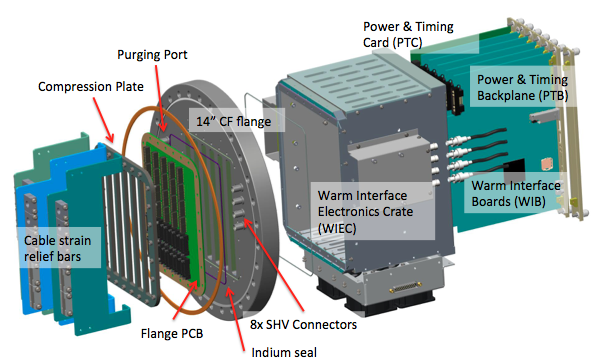
\includegraphics[width=0.9\linewidth]{sp-tpcelec-flange.png}
\end{dunefigure}

The \dword{wib} 
receives the system clock and control signals from the
timing system and provides processing and further distribution of those signals to four
\dwords{femb}. 
It also receives high-speed data signals from the same four 
\dwords{femb} and transmits them to the \dword{daq} system over optical
fibers. The data signals from the \dwords{femb} are recovered on the \dword{wib} with commercial 
equalizers. The \dwords{wib} are attached directly to the \dword{tpc}
\dword{ce} \fdth on the signal flange. The \fdth board is a \dword{pcb} 
with connectors to the cold signal and \dword{lv} power cables fitted
between the compression plate on the cold side and sockets for
the \dword{wib} on the warm side. Cable strain relief for the cold cables is 
provided from the back end of the \fdth.

The \dword{ptc} provides a bidirectional fiber interface to the
timing system. The clock and data streams are separately fanned out to the 
five \dwords{wib} as shown in Figure~\ref{fig:tpcelec-wib-timing}. The 
\dword{ptc} fans the clocks out to the \dwords{wib} over the \dword{ptb}, which is a 
passive backplane attached directly to both. A clock-data separator on the 
\dword{wib} separates the signal received from the timing system into clock and data. 
Timing endpoint firmware for receiving and transmitting 
the clock is integrated into the \dword{wib} \dword{fpga} (the Altera 
Arria V\footnote{Altera Arria\texttrademark{} V, 
\url{https://www.altera.com/products/fpga/arria-series/arria-v/overview.html}.} was used for \dword{pdsp}). 
The \dword{spmod} timing system, described in Section~\ref{sec:sp-daq:design-timing}, 
is a further development of the \dword{pdsp} system and is expected to have nearly identical 
functionality at the \dword{wib} endpoint.

\begin{dunefigure}
[PTC and timing distribution to the WIB and FEMBs]
{fig:tpcelec-wib-timing}
{\Dword{ptc} and timing distribution to the \dword{wib} and \dwords{femb} used in \dword{pdsp}.}
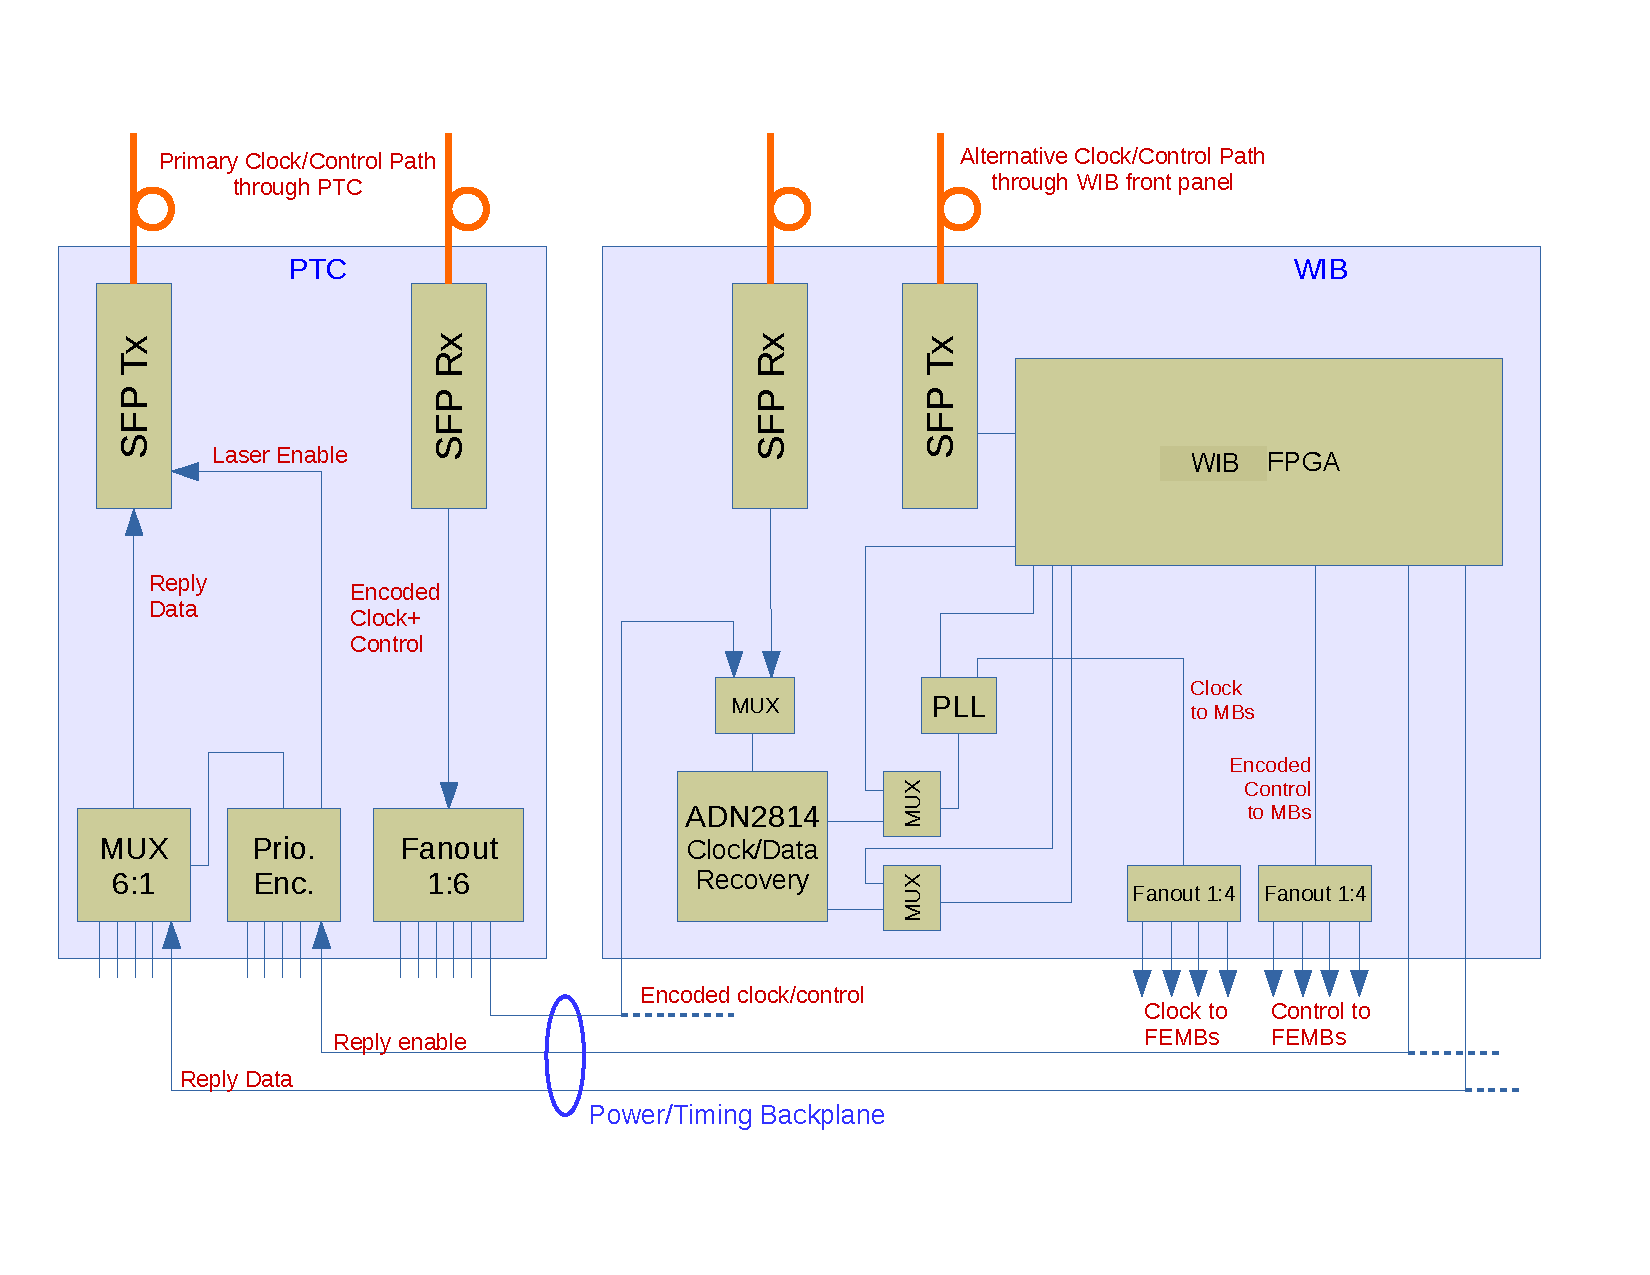
\includegraphics[width=0.75\linewidth]{sp-tpcelec-wib-timing-v2.pdf}
\end{dunefigure}

The \dword{ptc} %also 
receives \SI{48}{V} \dword{lv} power for all \dword{tpc} electronics %cold electronics 
connected through the \dword{tpc} signal flange: 
one \dword{ptc}, five \dwords{wib}, and \num{20}~\dwords{femb}. 
The \dword{lv} power is then stepped down to \SI{12}{V} via 
a \dword{dc}-\dword{dc} converter on the \dword{ptc}. The output 
of the \dword{ptc} converters is filtered with a common-mode choke 
and fanned out on the \dword{ptb} to each \dword{wib}, which provides the 
necessary \SI{12}{V} \dword{dc}-\dword{dc} conversions and fans
the \dword{lv} power out to each of the  \dwords{femb} supplied 
by that \dword{wib}, as shown in Figure~\ref{fig:tpcelec-wib-power}. 
The output of the \dword{wib} converters is further filtered by a 
common-mode choke, and each voltage line provided to the \dwords{femb}
is individually controlled, regulated, and monitored.

\fixme{ Figures 4.32 and 4.33 are still the old ProtoDUNE ones. We are working on replacement ones.}
\begin{dunefigure}
[Low voltage power distribution to the WIB and FEMBs]
{fig:tpcelec-wib-power}
{\dword{lv} power distribution to the \dword{wib} and \dwords{femb} 
for \dword{dune} \dword{spmod}. This will be modified for the 
\dword{spmod} to provide the required voltage or voltages 
depending on which \dwords{asic} are used on the \dwords{femb}. 
In particular, the voltages to the \dword{femb} \numrange{0}{3} 
will change as the \dword{pdsp} \dword{fpga} is replaced by \dword{coldata}. }
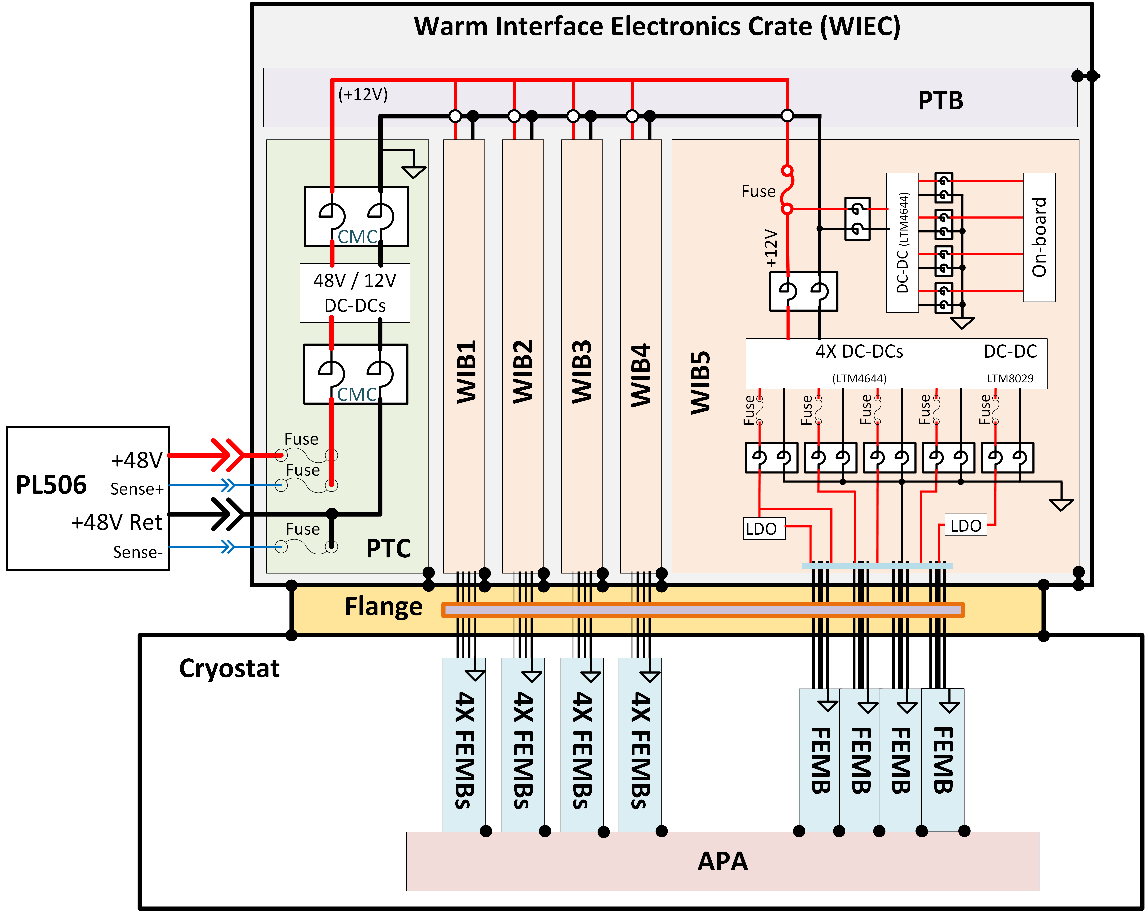
\includegraphics[width=0.65\linewidth]{sp-tpcelec-wib-power.pdf}
\end{dunefigure}

Because the \dwords{wib} can provide local power to the \dword{femb} 
and real-time diagnostic readout of all channels, each \dword{tpc} electronics 
system for each \dword{apa} is a complete, stand-alone readout unit. 
The \dwords{femb} and cold cables are shielded inside the cryostat, 
and the \dwords{wib} and \dword{ptc} are shielded inside the Faraday 
cage of the \dword{wiec}, with only shielded power 
cables and optical fibers connecting to external systems.

\begin{dunefigure}
[Warm interface board]
{fig:tpcelec-dune-wib}
{\dword{wib}. Note that front panel inputs include 
a LEMO connector and alternate inputs for \dword{lv} power and timing.}
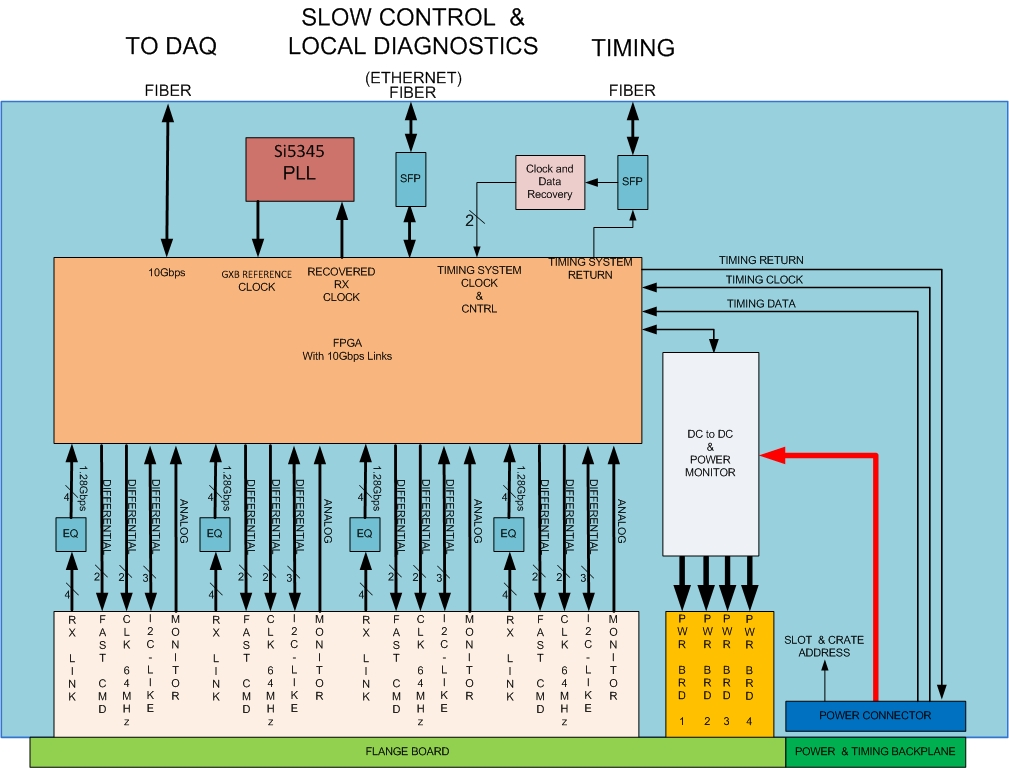
\includegraphics[width=0.8\linewidth]{sp-tpcelec-dune-wib.jpg}
\end{dunefigure}

As shown in Figure~\ref{fig:tpcelec-dune-wib}, the \dword{wib} can 
receive \dword{lv} power in the front panel and distribute it directly 
to the \dword{femb}, bypassing all \dword{dc}-\dword{dc} converters.
It can also receive the encoded system timing signals over bidirectional 
optical fibers on the front panel and process them using either
the on-board \dword{fpga} or clock synthesizer chip to provide the 
clock required by the \dword{tpc} electronics. The baseline \dword{asic} design 
currently uses 8b/10b encoding; if the \dword{slac} \dword{cryo} 
\dword{asic} is selected for the \dword{dune} \dword{spmod}, 
12b/14b encoding will be used instead of 8b/10b.

The \dword{fpga} on the \dword{wib} will have transceivers that can 
drive the high-speed data to the \dword{daq} system up to
\SI{10}{Gbps} per link, indicating that all data from
two \dwords{femb} (2$\times\SI{5}{Gbps}$) could be transmitted 
on a single link. The \dword{fpga} will have an additional 
transceiver I/O for an optical \SI{1}{Gbps} Ethernet connection, which 
provides real-time monitoring of the \dword{wib} status to the slow control system.

For system tests, discussed later in Section~\ref{sec:fdsp-tpcelec-qa-facilities},
the \dword{wiec}, \dword{wib}, and \dword{ptc} developed for \dword{pdsp}
are being used. A special version of the \dword{wib} has been developed
for use with \dwords{femb} equipped with the \dword{cryo} \dword{asic},
that require a different power and clock distribution scheme. Plans are
being put in place to redesign the \dword{wib}, and eventually make 
minor changes also to the \dword{ptc} and the \dword{wiec}, to use 
less expensive \dwords{fpga} and to be able to program independently
the voltage rails used to provide power the \dwords{femb}. This will include
the possibility of setting independent voltage and current limits on each power
rail. The current \dword{pdsp} version of the \dword{wib} already foresees
the possibility of monitoring and turning on and off independently the
various voltage rails. Another feature that we are planning to insert in
the \dword{wib} is the possibility of measuring the delay of the propagation
of the clock signal between the \dword{wib} and the \dwords{femb}. With
this feature it will be possible to align in situ the sampling time of different
\dwords{femb} to a precision of a few ns, without relying on the 
measurement of the cable lengths, which is the method that was used
in \dword{pdsp}.


%%%%%%%%%%%%%%%%%%
\subsection{Timing Distribution and Synchronization}
\label{sec:fdsp-tpcelec-design-timing}

The charge deposited on each wire of the \dword{apa}s installed 
in the \dword{dune} \dword{spmod} is digitized at a frequency of
$\sim\,\SI{2}{MHz}$, as discussed in 
Section~\ref{sec:fdsp-tpcelec-overview-requirements}. This requires
that the \dword{tpc} electronics be synchronized to a level of the order of \SI{10}{ns}, which is
much smaller than the time difference between two charge samples.
This level of error in the synchronization between the sampling time of different
\dwords{femb} contributes negligibly to the expected resolution % 
of the reconstructed space points measurement,
both in the \dword{apa} plane and along the drift distance.
The timing distribution and synchronization system for the 
\dword{spmod} is described in Section~\ref{sec:sp-daq:design-timing}.
Each \dword{wiec} has a bidirectional optical connection with the
timing system in the \dword{ptc}. Inside the \dword{ptc} the optical
signal from the timing system is converted, as discussed in the previous
section, to an electrical signal and distributed via the backplane to
the \dwords{wib} that constitute an endpoint for the timing distribution
system. Each \dword{wib} contains a standalone jitter-reducing \dword{pll} 
that forwards the clock to all the \dwords{femb}. The
\dword{fpga} contained inside the \dword{wib} implements the 
protocol~\cite{bib:docdb1651,bib:docdb11233} for aligning
the phase of the clock at the endpoint of the distribution tree.

The timing distribution and synchronization system ensures that
all the \dwords{wib} are synchronized to within $\sim\SI{3}{ns}$. 
One possible way of synchronizing the \dwords{femb} is the one
that was used in \dword{pdsp}, which relies on the fact that 
that all the cables connecting the \dwords{wib} to the
\dwords{femb} have approximately the same length (a length 
difference of \SI{0.5}{m} corresponds to a difference in the
sampling time of \SI{2.5}{ns}). The same approach could be used
for the \dword{dune} \dword{spmod}, correcting for the top-bottom 
\dword{apa} cable length difference (corresponding to $\sim\,\SI{65}{ns}$) 
inside the \dword{fpga} of the \dword{wib}. The exact correction
factor could be obtained by measuring the time propagation 
difference for a sample of short and long cables prior to the 
installation of the \dwords{femb} on the \dwords{apa}. 
Synchronizing the \dword{ce} with the \dword{pds} requires one
additional time constants that correspond to the transit 
time of the Fast Command sent from the \dword{wib} to
\dword{coldata} and from there to the \dword{coldadc},
which includes the propagation time along the cables
(\SI{45}{ns} for the \SI{9}{m} long cables to the top \dword{apa}s
and \SI{110}{ns} for the \SI{22}{m} long cables to the bottom \dword{apa}s) 
plus the propagation time inside the \dwords{asic}. This overall 
time constant can be obtained offline from the data, but it represents 
at most a correction of $\mathcal{O}(\SI{150}{\mu m})$ on the 
position of a track along the drift distance.
Instead of relying on cable measurements we are also considering
the addition of a timer inside the \dword{wib}'s \dword{fpga},
to measure the transit time of a command
sent to the \dword{femb} and its corresponding return
message. This study will help us understand whether the 
relative phases of the \dword{femb} and the \dword{wib} 
can be aligned more precisely.

The communication between the \dword{wib} and the \dword{daq} 
backend is asynchronous and the \num{64}-bit time-stamp, that
is used to indicate the time at which the signal waveform was
sampled~\ref{sec:sp-daq:design-timing}, is inserted in the data frame
in the \dword{wib}'s \dword{fpga}. 
For the three-\dwords{asic} solution, the communication
from the \dword{femb} to the \dword{wib} is also
asynchronous and a \num{8}-bit time stamp is sent to
count the number of \dword{adc} samples (triggered by
the \dword{femb} with a ``Fast Command'' signal) from the last
``Sync'' signal, as discussed in Section~\ref{sec:fdsp-tpcelec-design-femb-coldata}.
This \num{8}-bit time stamp is used only to ensure
that the \dword{femb} and the \dword{wib} are
still in sync. 

In contrast to the three-\dwords{asic} solution, 
in the \dword{cryo}-based \dwords{femb} solution 
the communication between the \dword{femb} and 
\dword{wib} is entirely synchronous, using a \SI{56}{MHz} 
clock. In order to properly align the phase of the
\dword{adc} sampling for the top and bottom \dword{apa}s,
appropriate delays must be added to the sampling
command in the \dword{wib}'s \dword{fpga}. 
The requirements listed above for synchronizing 
the \dword{ce} relative to the \dword{pds} remain
valid for this case. 

%%%%%%%%%%%%%%%%%%%%%%%%%%%%%%%%%%%
\subsection{Services on Top of the Cryostat}
\label{sec:fdsp-tpcelec-design-services}

A fully-loaded \dword{wib} (one \dword{wib} plus four \dwords{femb}) 
requires \SI{12}{V} and draws \SIrange{4.3}{4.7}{A}, including the
power required by the \dword{fpga} and the optical components (the range 
covers the difference between upper and lower \dword{apa}, and operation
at \lntwo and room temperature). In 
\dword{pdsp} the full electronics for one \dword{apa} (one \dword{ptc}, 
five \dwords{wib}, and \num{20} \dwords{femb}) requires \SI{12}{V} and 
draws \SIrange{22}{24}{A}, for a total power of approximately 
\SI{240}{W}. 

The \dword{lv} power is delivered at \SI{48}{V} to the \dword{ptc}, 
so each \dword{lv} power mainframe is chosen to bracket that value; 
each has roughly \numrange{30}{60}{V}, \SI{13.5}{A}, \SI{650}{W} 
maximum capacity per \dword{apa}. Using \num{10}AWG cable, and assuming
a distance of \SI{20}{m} between the \dword{lv} power supplies 
that are situated on the detector mezzanine and the most distant
cryostat penetration for a row of \dword{apa}s, a voltage
drop of at most \SI{1}{V} should occur along the cable with a required power of 
\num{335} to \SI{360}{W} out of \SI{650}{W} available.
At most $\sim\SI{150}{W}$ is dissipated inside the cryostat, and another
$\sim\SI{200}{W}$ is dissipated inside the \dword{wiec}, that is
air-cooled, and only a few watts are dissipated in the warm cables
that are located below the false flooring on top of the cryostat.
Multiplying by the total number of \dwords{wiec}, less 
than \SI{1}{kW} of power is dissipated in the cabling system 
over the entire surface of the cryostat. 

Four wires are used for each \dword{ptc} module; two \num{10}AWG, shielded, twisted-pair 
cables for the power and return; and two \num{20}AWG, shielded, twisted-pair 
cables for the sense. The primary protection is the over-current 
protection circuit in the \dword{lv} supply modules, which is set 
higher than the $\sim\SI{8}{A}$ current draw of the \dword{wiec}. 
Secondary sense line fusing is provided on the \dword{ptc}.  
Tests are being performed in \dword{pdsp} to check which is the
best scheme for connecting the shields of the power cables. In
\dword{pdsp} the shield of the warm power cables is connected to
ground on both the power supply side and on the \dword{ce} flange.
Other shield connection schemes are being investigated in \dword{pdsp}
and the connection scheme yielding the lowest read-out noise will be
used for \dword{dune}.

Switching power supplies controlled by the slow controls system provide
power to the heaters (\SI{12}{V}) and the fans (\SI{24}{V}) that are 
installed on the \dword{ce} flanges. Temperature sensors mounted on the
flanges, and power consumption and speed controls from the fans are 
connected to the interlock system that is part of the \dword{ddss}, in
addition to being monitored by the slow controls system.

Bias voltages for the \dword{apa} wire planes, the electron diverters,
discussed in Section~\ref{sec:fdsp-apa-intfc-apa}, 
and the last \dword{fc} electrodes are generated by supplies that are 
the responsibility of the \dword{tpc} electronics consortium.  The 
current from each of these supplies should be very close to zero in 
normal operation. However, the ripple voltage must be carefully 
controlled to avoid injecting noise into the \dword{fe} electronics.  
RG-58 coaxial cables connect the wire bias voltages from the bias voltage
supply to the standard \dword{shv} connectors that are machined directly 
into the \dword{ce} \fdth and insulated from the low voltage and 
data connectors.

Optical fibers are used for all connections between the \dwords{wiec} %, 
%which act as Faraday-shielded boxes,  <<--- already said
and the \dword{daq} and slow 
control systems.  The \dword{wib} reports its temperature 
and the current draw from each \dword{femb} to the slow control system, 
while the current draw for each \dword{apa} is monitored at the 
mainframe itself.

To support the electronics, fan, and heater power cables, as well 
as optical fibers on top of the cryostat, cable trays are installed
below the false flooring on top of the cryostat. These cable trays
run perpendicular to the main axis of the cryostat and connect the
three cryostat penetrations for one row of \dword{apa}s to the detector
mezzanine near the cryostat roof, as shown in Figure~\ref{fig:cryostat-roof}.
All the necessary \dword{lv} supplies and %, in addition to 
the bias
voltage supplies are installed in these racks. Patch panels for
the optical fiber plant used for the control and readout of the
detector are also installed on the detector mezzanine.

\begin{dunefigure}
[Services on top of the cryostat]
{fig:cryostat-roof}
{Services on top of the cryostat. The racks for the \dword{lv} power supplies are shown in blue.}
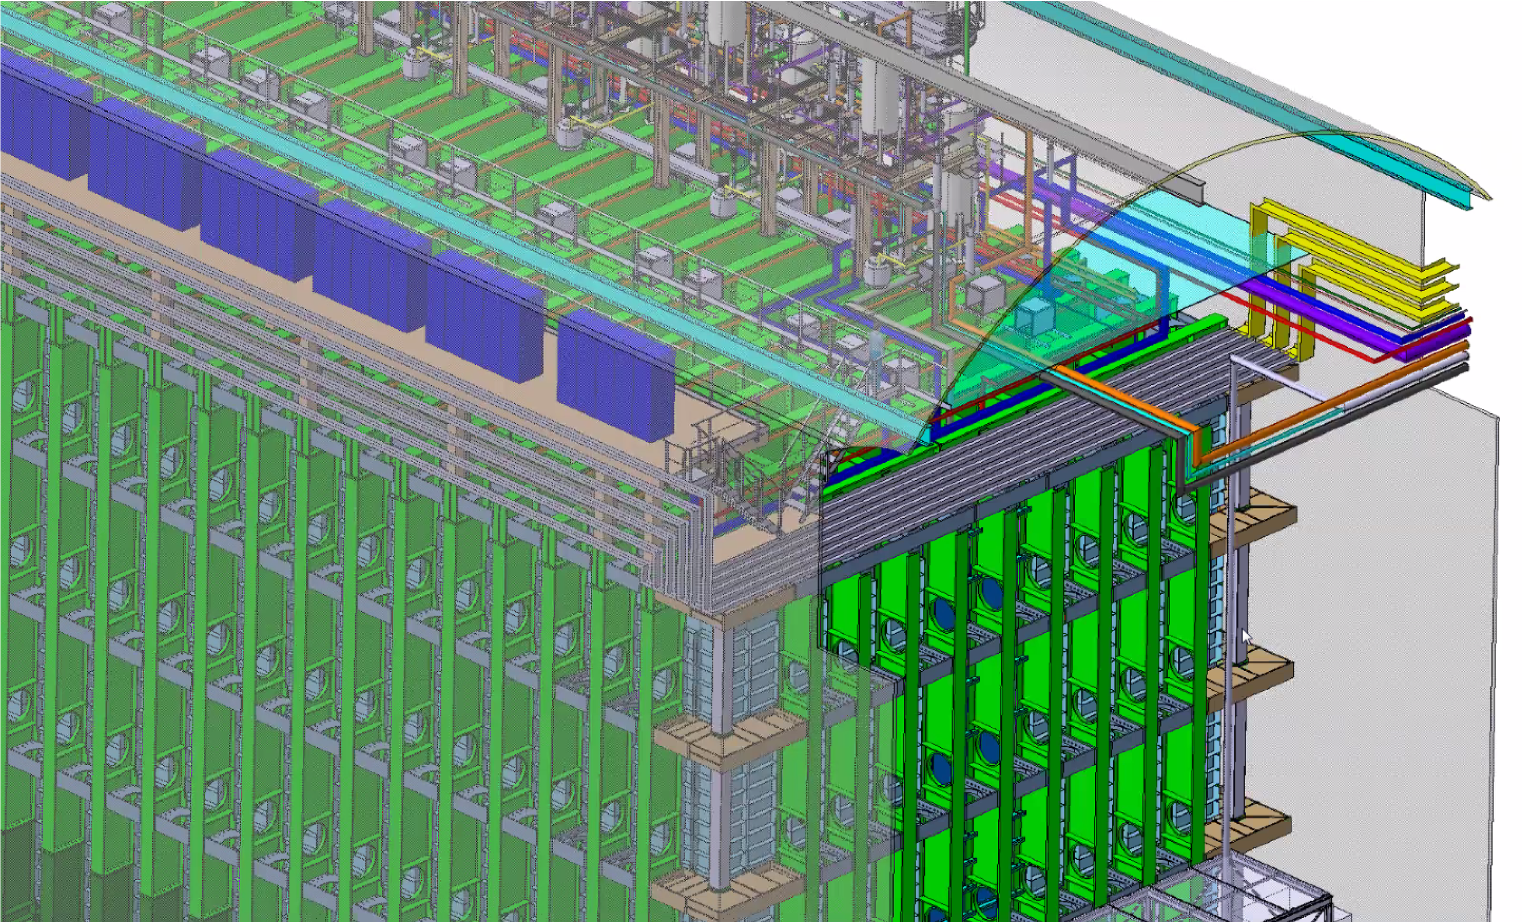
\includegraphics[width=0.9\linewidth]{sp-tpcelec-cryostat-top.png}
\end{dunefigure}

%%%%%%%%%%%%%%%%%%%%%%%%%%%%%%%%%%%
\subsection{ProtoDUNE-SP Results}
\label{sec:fdsp-tpcelec-overview-pdune}

The \dword{pdsp} detector is a 700-ton fiducial volume
\dword{lartpc} with 15,360 sense wires. 
The system was deployed in a beamline at the CERN Neutrino Platform 
in 2018 and continues to take cosmic event data into 2019. The goal of 
the \dword{pdsp} \dword{tpc} readout was to validate the concept 
and the design of the integrated \dword{apa}+\dword{ce} readout 
and measure the performance of the \dword{tpc} electronics system with components 
as close as possible in design to those in the final \dword{dune} \dword{tpc} readout.
In the case of the \dword{tpc} electronics, most of the detector components 
used in \dword{pdsp} are prototypes of the \dword{dune} ones discussed in the 
previous Sections. The major difference is the \dword{femb}, where an
early version of \dword{larasic} (P2) is used for the \dword{fe}, followed
by the first prototype (P1) of a different \dword{adc}, using the ``domino'' architecture 
and implemented in the \SI{130}{nm} technology, and by
a \dword{fpga} that provided the data serialization functionality.

Each of the six \dword{pdsp} \dword{apa}+\dword{ce}
readout units consists of 2,560 sense wires, of which 960 are \SI{6}{m} 
long collection wires and 1,600 are \SI{7.4}{m} long induction wires. 
Five of the six \dword{apa}s were tested in a full-scale cold box in 
cold gaseous nitrogen (GN$_2$) with a complete \dword{tpc} electronics readout system,  
identical to the one %on the detector, 
deployed in \dword{pdsp}, before installation in the cryostat,
while the sixth %one
 was installed without first going through the cold
box testing. Figure~\ref{fig:apa2-cycle} shows the measured noise, in 
electrons, for the collection (X) plane and the two induction (V, U) 
planes as well as the \dword{femb} temperature in the cold box as a 
function of the cold cycle time. At a stable temperature of 
\SI{160}{K} the \dword{enc} for all three wire planes is less than 500~e$^-$.

\begin{dunefigure}
[ProtoDUNE-SP APA \#2 ENC levels measured in GN$_2$ in the CERN cold box]
{fig:apa2-cycle}
{Left $y$ axis: Noise (in electrons) for U, V, and X (red, blue, and green 
curves) sense wire planes as a function of time (hours) for the APA \#2 cold 
cycle in GN$_2$ in the CERN cold box; right $y$ axis: temperature 
(orange curve) measured at the level of the \dword{fe} electronics.}
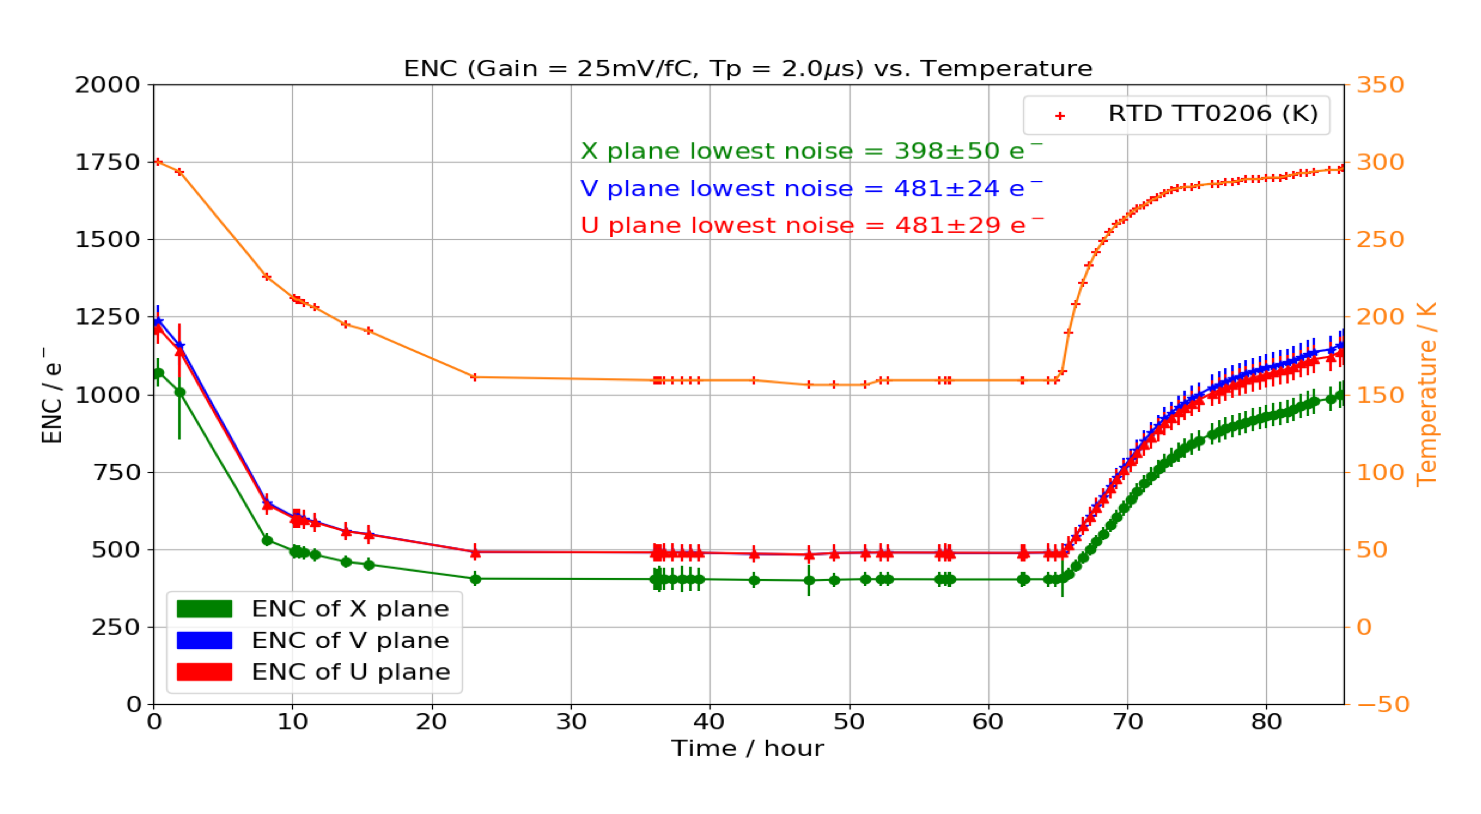
\includegraphics[width=0.95\linewidth]{sp-tpcelec-apa2.png}
\end{dunefigure}
After the cryostat was filled with \dword{lar} and the drift and wire 
bias voltages were set to their nominal values
99.7\% of the \dword{tpc} readout channels were live.
There is a total of 42 channels that are not responsive. Of these:
\begin{itemize}
\item{14 channels were identified based on tests performed prior
to the insertion of the \dword{apa} into the cryostat as having
no capacitive load on the \dword{fe} electronics, suggesting an open 
connection somewhere upstream  of the \dword{ce} system;}
\item{24 additional channels showed the same problem after the
cryostat was filled with \dword{lar} (three of these, all on the
first APA were already observed during testing in the cold box);}
\item{in four cases the \dword{fe} electronics is dead: two of these
channels appeared in tests performed after the cathode high
voltage was raised to \SI{120}{KV}, and two more
appeared when the high voltage reached \SI{160}{KV}.}
\end{itemize}

No further loss of readout channels has occurred since 
the end of September 2018. If this number is indicative
of the normal rate of channel loss, it would imply that
over the \dunelifetime of \dword{dune} operations at
most \num{0.5}\% of the readout channels would fail. A
similar upper limit can be obtained from the operational
experience of \dword{microboone}, considering also an
additional scale factor for the additional \dwords{asic}
immersed in \dword{lar} (in \dword{microboone} only
the \dword{fe} amplifier is in the liquid). Further 
operation of \dword{pdsp}, as well as operation of
\dword{sbnd} in the coming years, will provide additional
information on the long term stability of the active electronics
components immersed in \dword{lar}.

With the detector operating under nominal
conditions, the \dword{enc}
measured by the online monitoring program was approximately $\SI{550}{e^-}$ 
on the collection wires and approximately $\SI{650}{e^-}$ on the induction
wires, averaged over all operational channels. The noise increased
relative to the tests performed inside the cold box due to the 
larger dielectric constant of \dword{lar} relative to GN$_2$. 
These noise measurements 
are consistent with the 
ratio of the corresponding capacitances of the \dword{apa} wires. 
Figure~\ref{fig:apa3-noise} 
shows the \dword{enc} (in electrons) for all channels of one 
\dword{apa}+\dword{ce} readout unit. 
The collection channels with \dword{enc} larger than \SI{1500}{e$^-$} had a problem 
in the P1-\dword{adc} \dword{asic}; this problem had already been identified 
prior to their
installation on the \dwords{femb}. The channels on all three planes 
with \dword{enc} smaller than \SI{300}{e$^-$} have an open connection somewhere in 
front of the \dword{ce} system. Figure~\ref{fig:ENC-all} summarizes
\dword{enc} levels in the entire \dword{pdsp} detector both before and
after the application of a simple common-mode filter similar
to the one used in \dword{microboone}~\cite{Acciarri:2017sde};
an improvement of roughly 100~e$^-$ is seen on all planes. 

\begin{dunefigure}
[TPC ENC levels measured at ProtoDUNE-SP after \lar fill]
{fig:apa3-noise}
{\dword{enc} (in electrons) for all U, V, and X (red, blue, and green curves) sense 
wire planes for one \dword{pdsp} \dword{apa} %with the detector in 
under nominal operating 
conditions.}
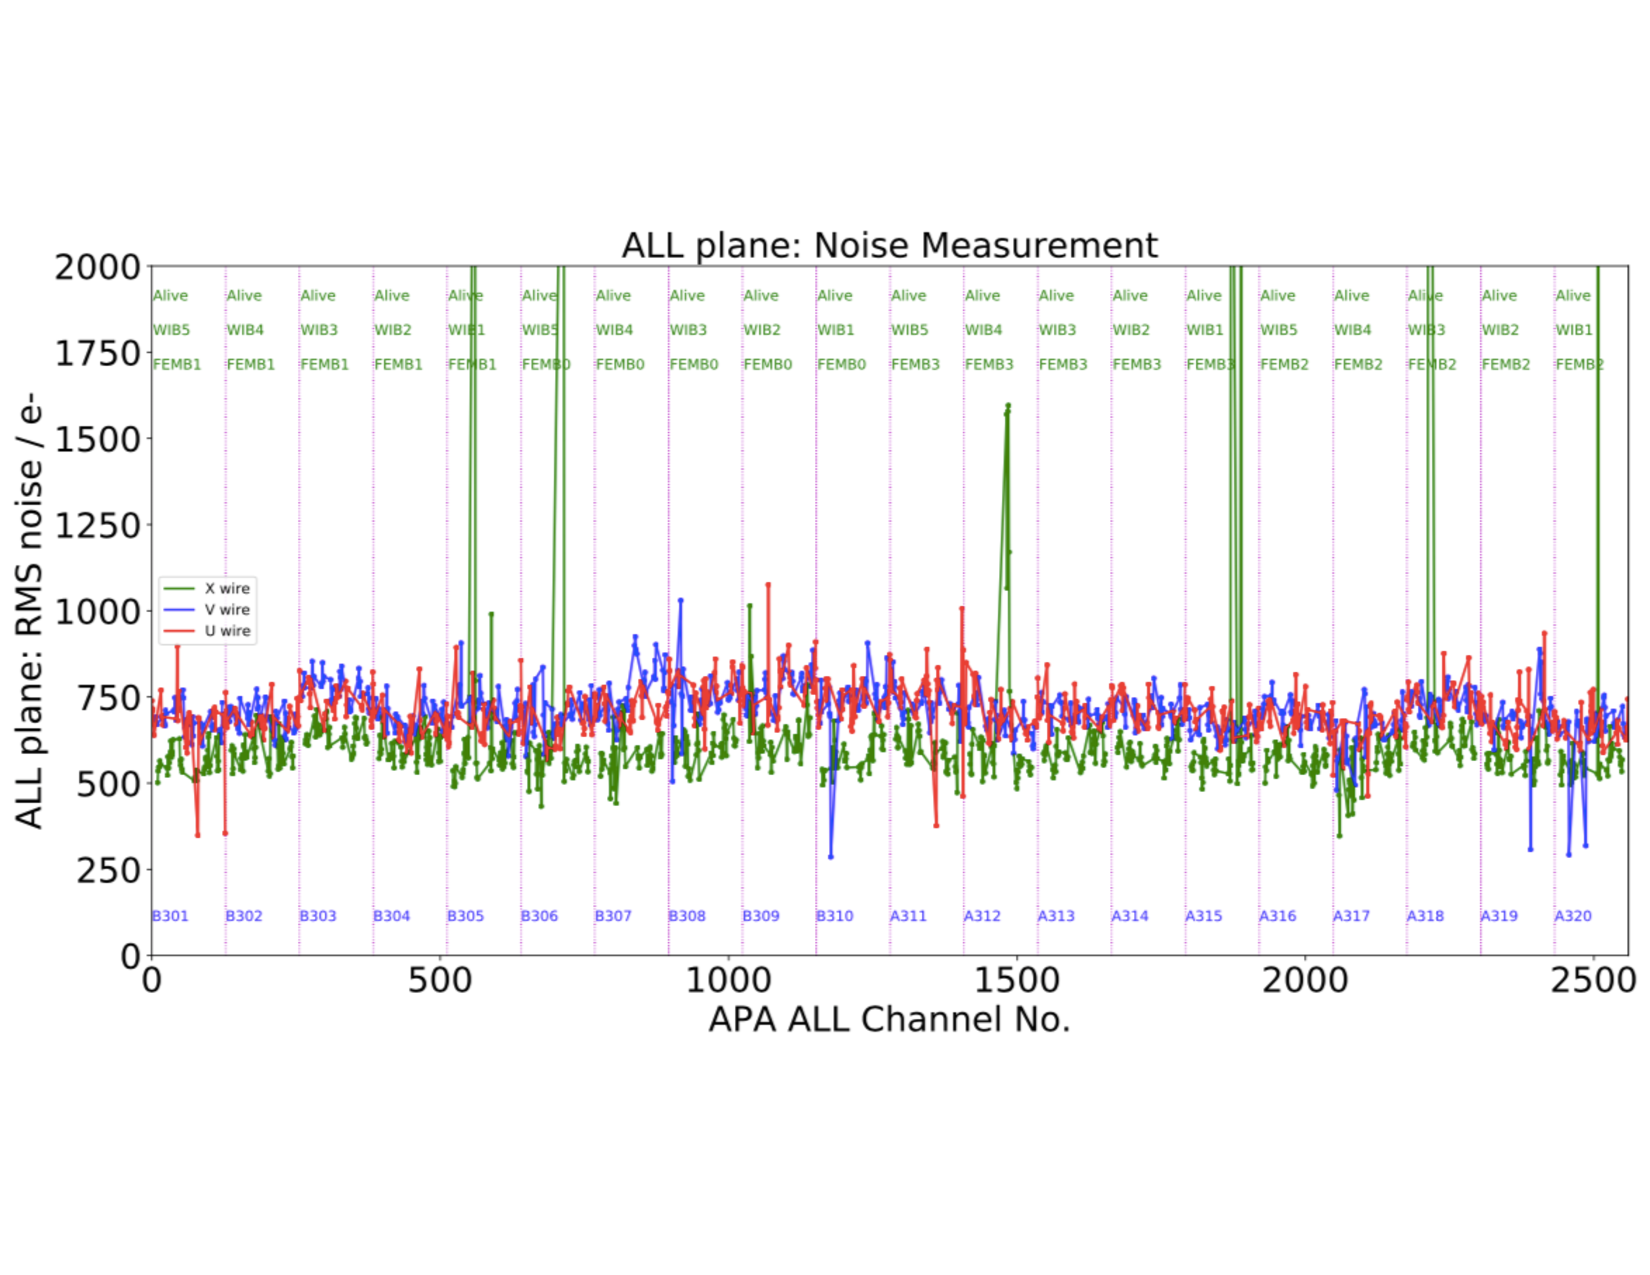
\includegraphics[width=0.9\linewidth]{sp-tpcelec-apa3-enc.pdf}
\end{dunefigure}

\begin{dunefigure}
[TPC ENC levels for all channels of the ProtoDUNE-SP detector]
{fig:ENC-all}
{\dword{enc} levels (in electrons) for all channels of the \dword{pdsp} detector, both
before and after the application of a simple common-mode filter.}
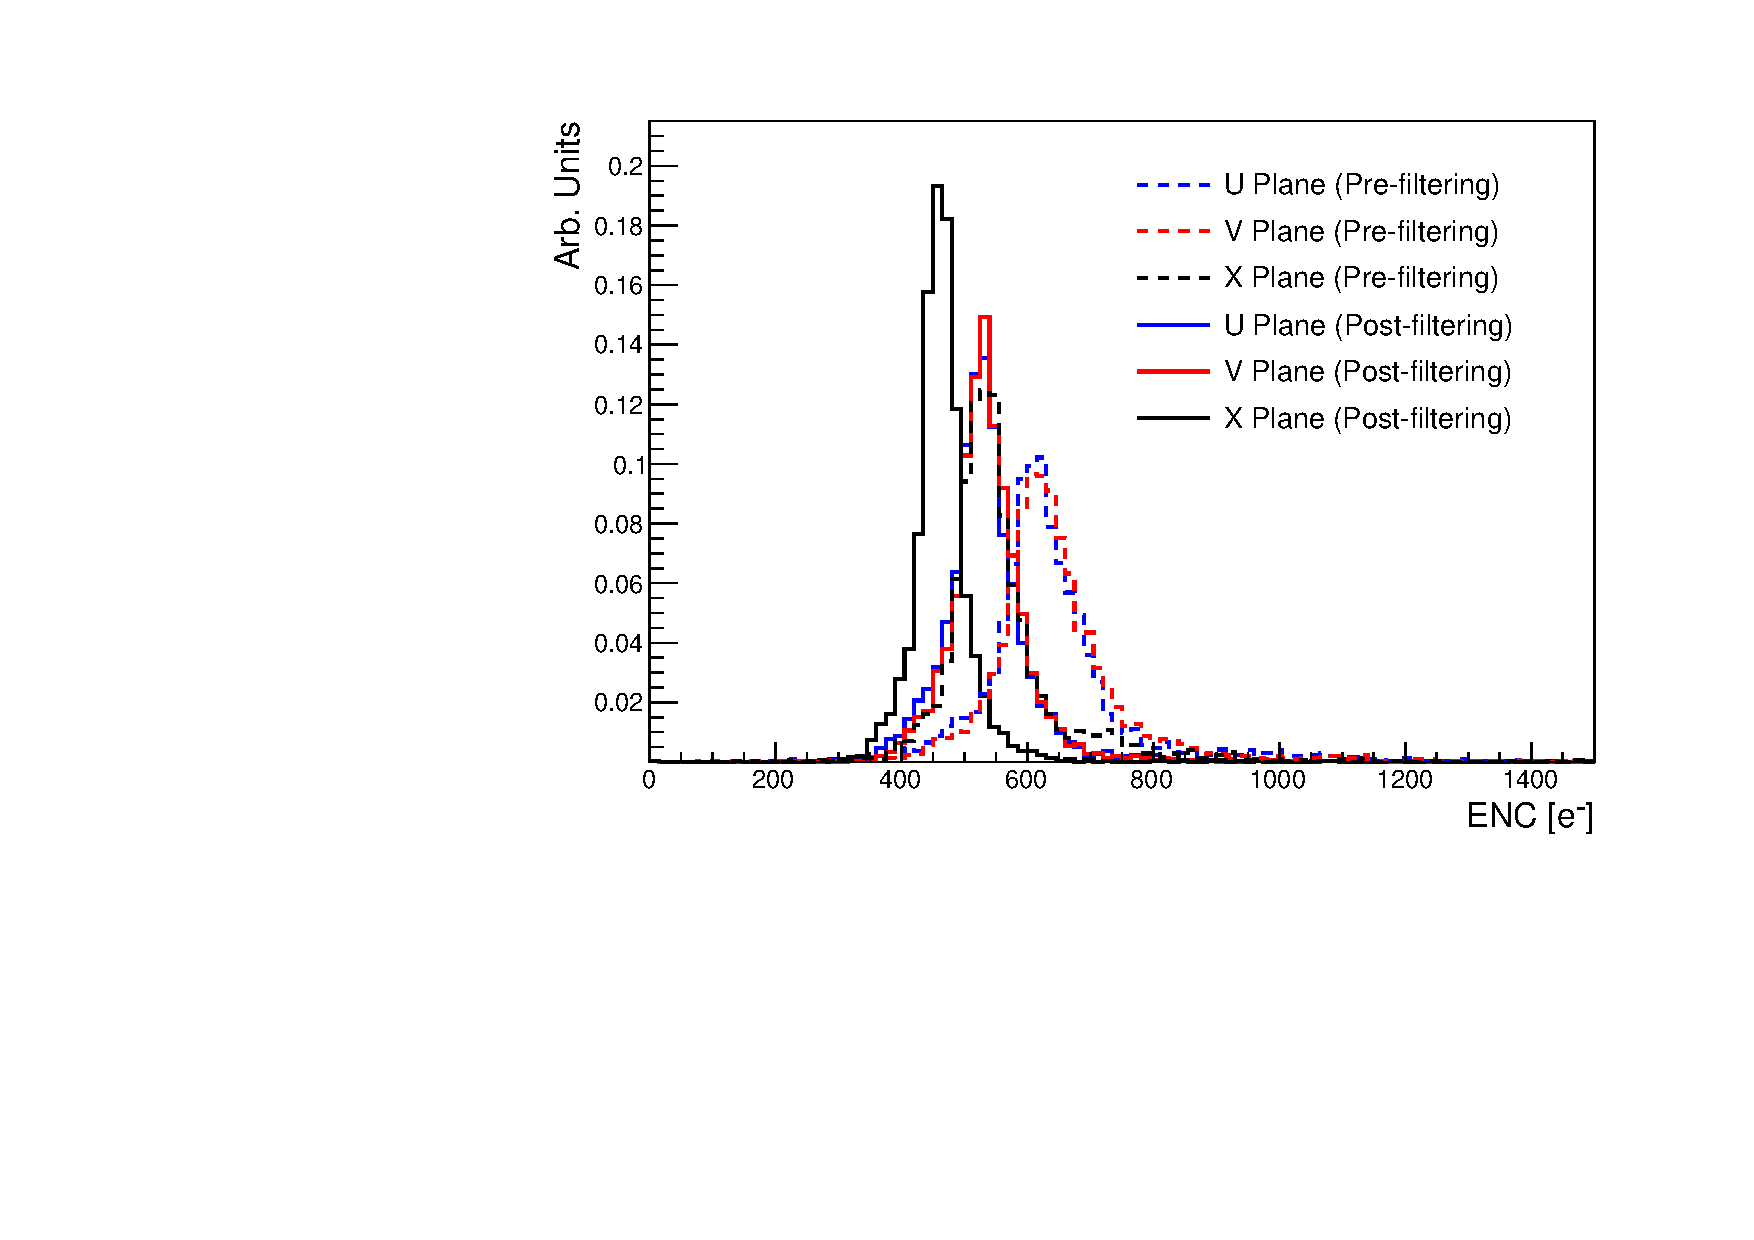
\includegraphics[width=0.99\linewidth]{sp-tpcelec-ENC-Combined.pdf}
\end{dunefigure}

The overall performance of the \dword{ce} system in 
\dword{pdsp} satisfies the 
\dword{ce} noise specification %requirements 
for the \dword{spmod} %\dword{fd} 
listed in Section~\ref{sec:fdsp-tpcelec-overview-requirements}. 
A comparison of the raw data from 
a \dword{pdsp} event (Figure~\ref{fig:pdsp-display}) to 
that from a \dword{microboone} event (Figure~\ref{fig:microboone-display}~\cite{Acciarri:2017sde}) 
demonstrates the improvements achieved in \dwords{lartpc} performance. 
The \dword{pdsp} event was collected very early in the data taking
period when the charge collection efficiency was still limited
by the amount of impurities in the \dword{lar}; it shows very little
noise and appears to be of the same quality as the \dword{microboone}
event display after offline noise removal. 

\begin{dunefigure}
[Raw data from a ProtoDUNE-SP event]
{fig:pdsp-display}
{Display of the charge deposited on the collection wires ($x$-axis) as
a function of the drift time ($y$-axis) for a \dword{pdsp} event 
that includes two electromagnetic showers and a four-prong interaction.
The color associated with each time sample on the \dword{apa}
wires gives a measurement of the charge measured by the \dword{ce}
readout, increasing from the smallest values (blue) to the largest
ones (red).}
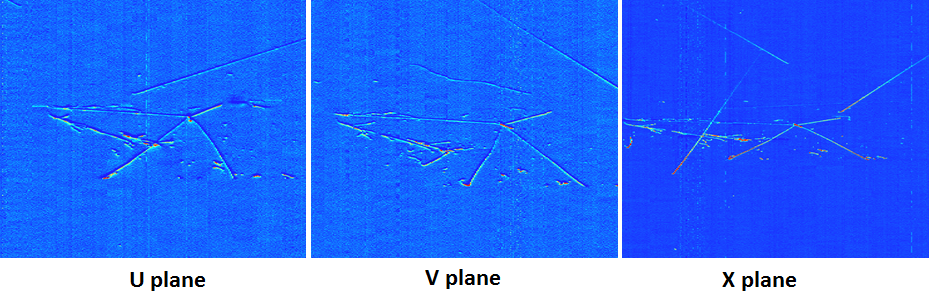
\includegraphics[width=1.0\linewidth]{sp-tpcelec-4prongdisplay.png}
\end{dunefigure}

\begin{dunefigure}
[Raw data from a MicroBooNE event]
{fig:microboone-display}
{\dword{microboone} \twod event display of the V plane from run 3493 
event 41075 showing the raw signal (a) before and (b) after offline 
noise filtering. A clean event signature is recovered once all the 
identified noise sources are subtracted~\cite{Acciarri:2017sde}.}
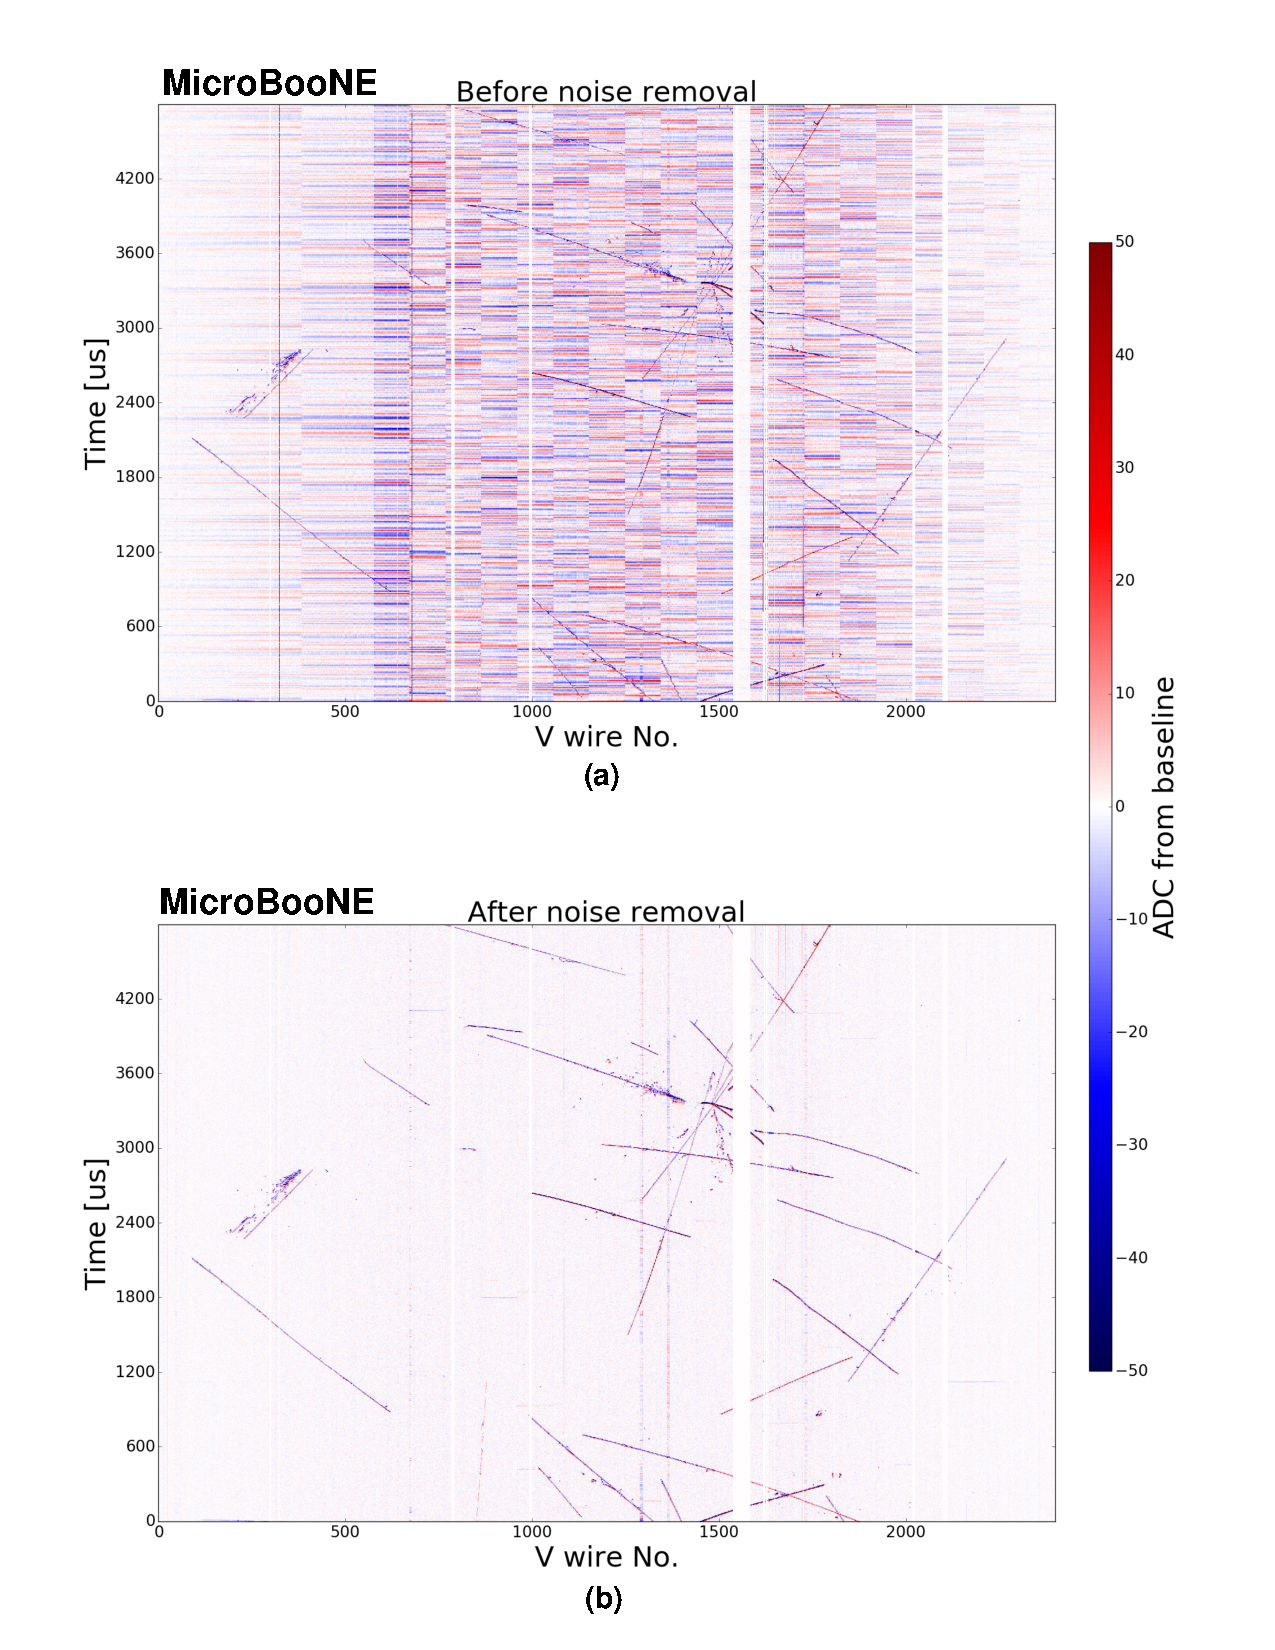
\includegraphics[width=0.9\linewidth]{sp-tpcelec-microBoone_display.pdf}
\end{dunefigure}

\begin{dunefigure}
[Signal over noise for muon tracks reconstructed in ProtoDUNE-SP]
{fig:pdsp-signalovernoise}
        {Signal over noise for reconstructed muon tracks in \dword{pdsp}.}
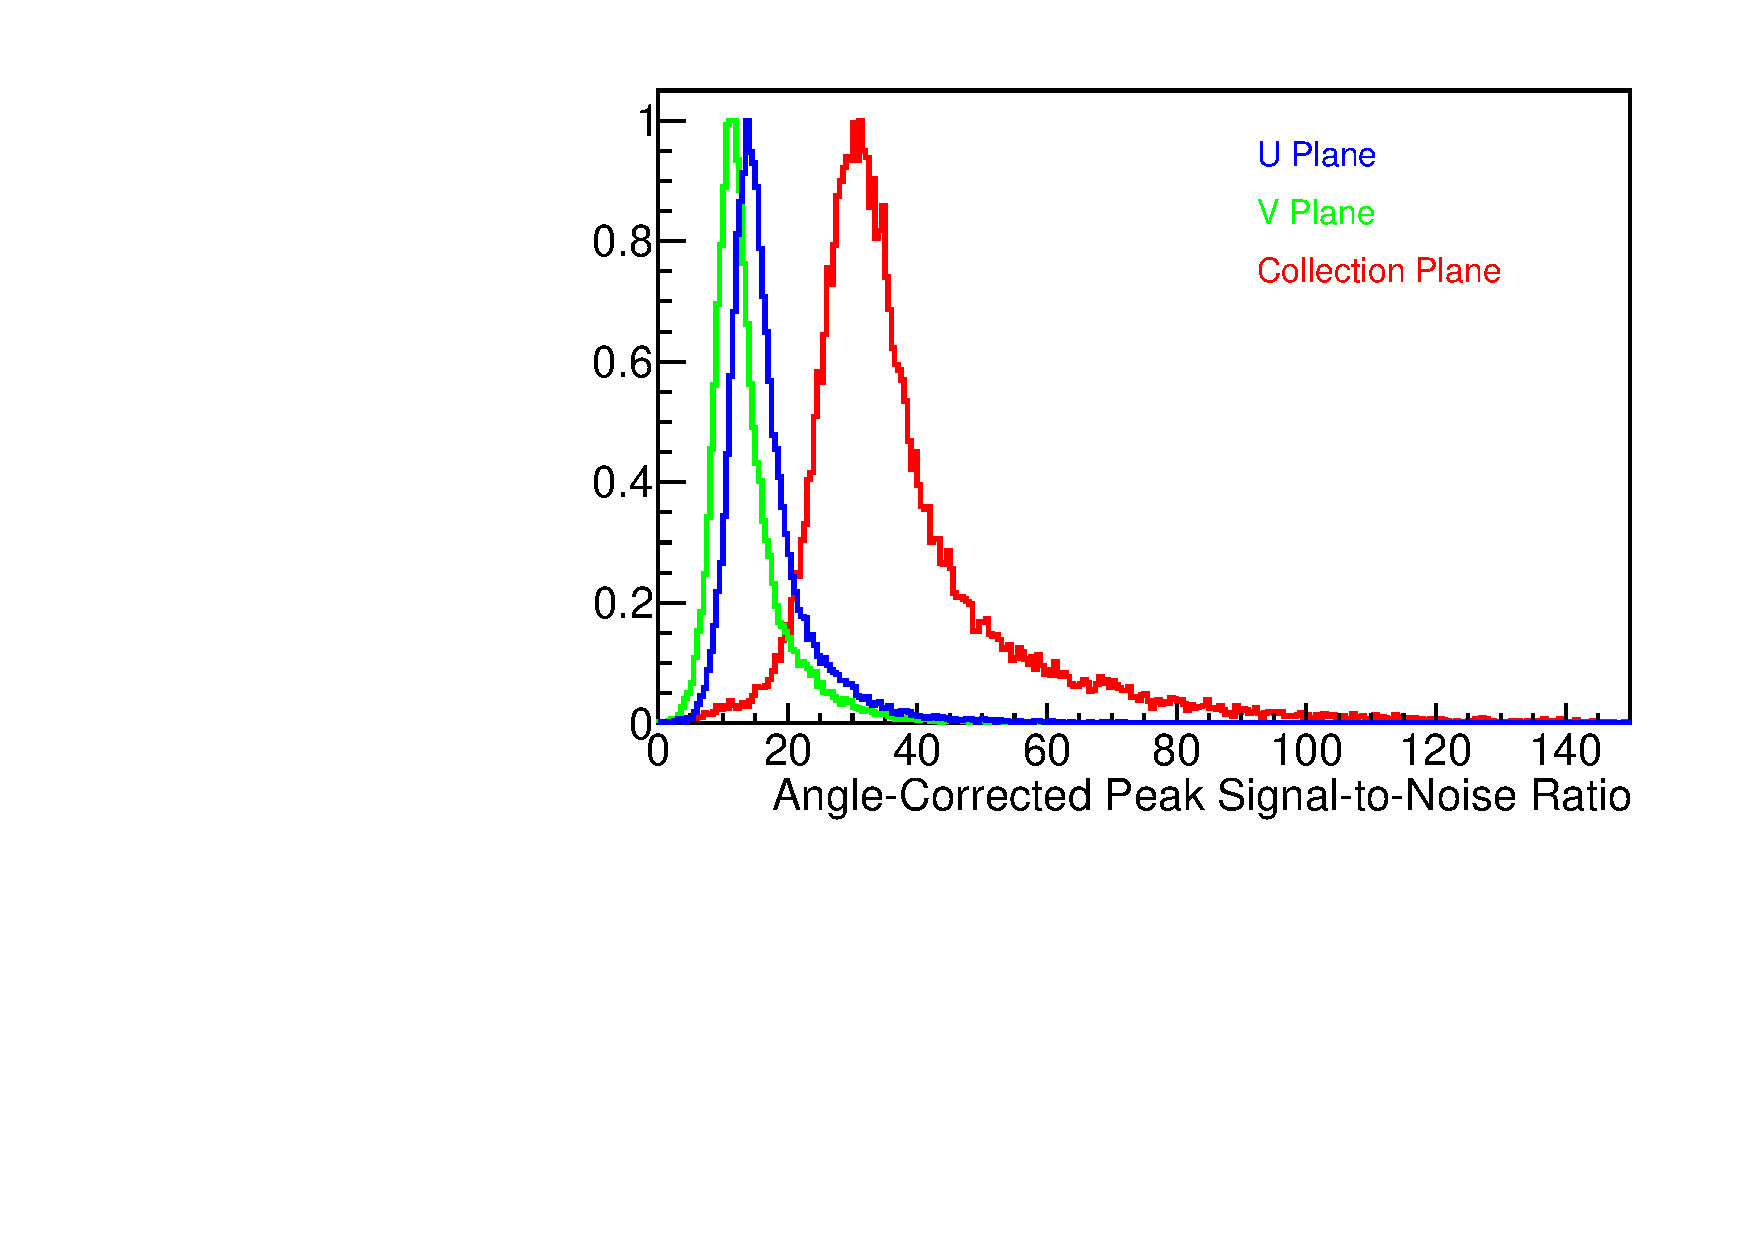
\includegraphics[width=0.85\linewidth]{sp-tpcelec-tracks-signal-over-noise.pdf}
\end{dunefigure}

The \dword{snr} has been evaluated a selected cosmic muon sample, with tracks
crossing the \dword{lar} volume at shallow angle with respect to the anode plane and
large angle with respect to the direction of the wires in the plane considered
for \dword{snr} characterization. The charge deposited on each wire in a plane is evaluated
using the pulse height (peak) of the hit found in the raw waveform.
A correction taking into account different relative angle between track and wire
direction has been applied to normalize the hit response. The noise value is extracted
from a fitted Gaussian width on the pedestal distribution of the waveform baseline of the
wire. The electric field in the \dword{tpc} volume was at nominal level of \SI{500}{V/cm},
and the \dword{lar} purity for the runs considered in this analysis was about \SI{5.5}{ms}
as measured by the purity monitors, corresponding to $\sim35$\% charge loss due to
attachment for tracks close to the cathode. No noise filtering has been applied for
this measurement. In addition, we ignored the effect of the space charge, that introduces
distortions of the electrical field in the \dword{tpc} volume that may local change the
recombination factor and therefore affect the \dword{snr} value. The distribution of
the \dword{snr} for all the wires in the sample of muon tracks considered is shown
in Figure~\ref{fig:pdsp-signalovernoise}. For the collection plane the mean value
of the distribution of \dword{snr} is 38, while for the two induction planes it is
14 (U) and 17 (V). A more accurate \dword{snr} estimate will be performed again as
soon as the effects of space charge are fully understood.

%%%%%%%%%%%%%%%%%%%%%%%%%%%%%%%%%%%
\subsection{ProtoDUNE-SP Lessons Learned}
\label{sec:fdsp-tpcelec-overview-lessons}

As discussed in Section~\ref{sec:fdsp-tpcelec-overview-pdune}, the initial 
data from \dword{pdsp} show that the \dword{spmod} can meet the noise specification. 
The experience with the \dword{tpc} electronics in \dword{pdsp} nonetheless motivates 
several improvements to the \dword{tpc} electronics system design, some of which
have already been implemented and discussed in the previous Sections.
A complete list of the lessons learned from the construction, testing, integration,
installation, commissioning of the \dword{tpc} electronics detector components
is available~\cite{bib:docdb12367}. This reference also discusses
the plans and timeline for addressing the issues observed in \dword{pdsp}. 
This \dword{tdr} section and the following cover only the main issues 
and the plans for their resolution and for implementation in the \dword{spmod}. 

During the commissioning of \dword{pdsp}, violations of the
grounding rules described in Section~\ref{sec:fdsp-tpcelec-design-grounding}
have been observed with one of the readout
boards for the \dword{pds}, and with the cameras immersed
inside the \lar. The power supply used to provide the \dword{hv} to the 
cathode plane has also been observed
to cause noise inside the detector and has been replaced.
The overall success of \dword{pdsp} owes much to the fact that the
grounding rules were properly implemented
and that any violation was discovered and addressed during
the commissioning.

The main problem with the \dword{pdsp} \dword{tpc} electronics readout is in the
P1-\dword{adc} \dword{asic}. This problem was observed as early as 2017 
while these \dwords{asic} were being tested prior to their installation
on the \dwords{femb}. The ``domino'' architecture~\cite{dominoADC} used in this design relies on
excellent transistor matching, which unfortunately 
is worse at \dword{lar} temperature. In \dword{pdsp} this problem
results a fraction (about \num{3.2}\%) of the readout channels having a fixed value for some of
the \dword{adc} bits, independent of the input voltage. In a majority
of the cases an approximate value for the charge can be obtained via
interpolation. For about \num{0.9}\% of the channels the problem is
so severe that the only solution is to remove the channels from the
analysis, resulting in a loss of efficiency. This problem prompted us to abandon
this design and to develop the completely new \dword{coldadc}, to
adapt the \dword{cryo} \dword{asic} for use in \dword{dune}, and to
follow the approach of the \dword{sbnd} Collaboration and consider
also the \dword{cots} \dword{adc} option.

Initial analysis of the \dword{pdsp} data has uncovered a new problem with \dword{larasic} 
that occurs when $>$\SI{50}{fC} is collected over a period of \SIrange{10}{50}{$\mu$s}, 
when the baseline configuration of the amplifier for the collection wires is used. 
The feedback mechanism of the \dword{fe} amplifier stops working for several 
hundred $\mu$s. During this period, the readout does not function and signals 
following the large charge deposited can be completely lost. A ledge is observed 
in the output of the \dword{fe} amplifier, followed by a slow decay 
and a sudden turn-on of the amplifier.
Figure~\ref{fig:pdsp-ledge} shows an example of this behavior.

\begin{dunefigure}
[Pulse shape on a ProtoDUNE-SP wire showing the ledge effect]
{fig:pdsp-ledge}
{Waveform of an event showing the ledge following a large charge 
deposition, then a discharge and a final jump to the normal baseline.}
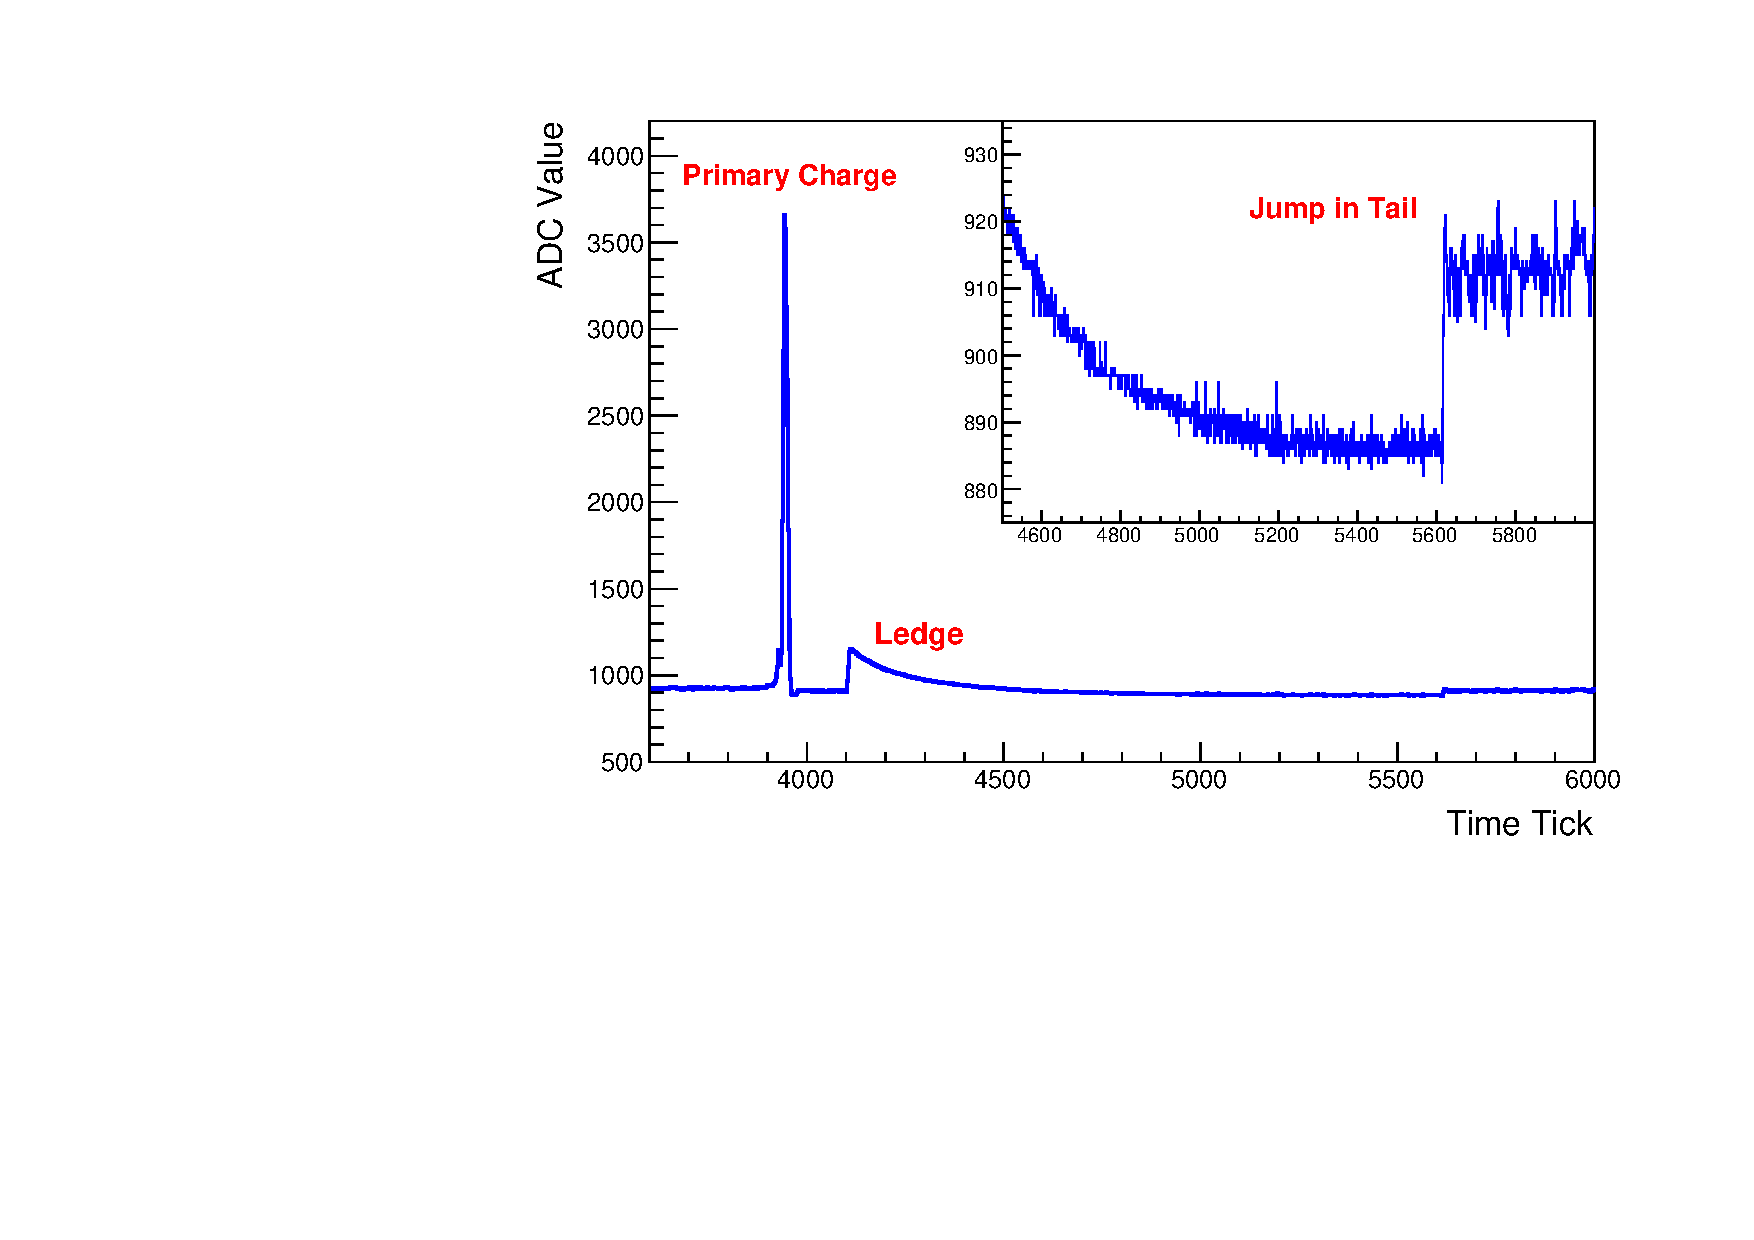
\includegraphics[width=1.0\linewidth]{sp-tpcelec-ledge.pdf}
\end{dunefigure}

This problem has been reproduced in the laboratory and is being actively 
studied. It affects all versions of \dword{larasic} fabricated after 
the one used for the \dword{microboone} experiment. The problem occurs 
when the threshold on the injected charge is small and therefore affects
with larger probability the collection wires, where the \SI{200}{mV} baseline 
is used, compared to the induction wires, that have a \SI{900}{mV} baseline.
After the problem and this difference between the two baselines were 
observed, the decision was taken to operate the \dword{ce} in \dword{pdsp} 
using the \SI{900}{mV} baseline also for the collection wires, sacrificing
the dynamic range. Data from the wires where the problem occurs can
be masked in analysis, resulting in a loss of efficiency. This problem 
affected a very small fraction of the events: with the \SI{200}{mV}
baseline about \num{0.1}\% of the waveforms were affected, and this
number became almost completely negligible after switching to the 
\SI{900}{mV} baseline. It should be
noted that the problem occurs more often in \dword{pdsp} 
than is expected in the \dword{fd}  \dword{spmod} due to the presence of 
cosmic rays traveling parallel to the \dword{apa} wires.
The problem could, however, affect the \dword{spmod}'s ability to detect
electromagnetic showers -- one of the main physics signals.
Section~\ref{sec:fdsp-tpcelec-overview-remaining} discusses the plans and timeline 
for addressing this issue in a new \dword{larasic} prototype.

\begin{dunefigure}
[Image of a connector for the cold cables lifted from the FEMB]
{fig:pdsp-femb-connector}
{Image of a connector for the cold readout and signal cables lifted from
the \dword{femb} due to the presence of excess epoxy on the 
connection between the cold cables and the printed circuit board
that acts as the ``male'' part of the connector.}
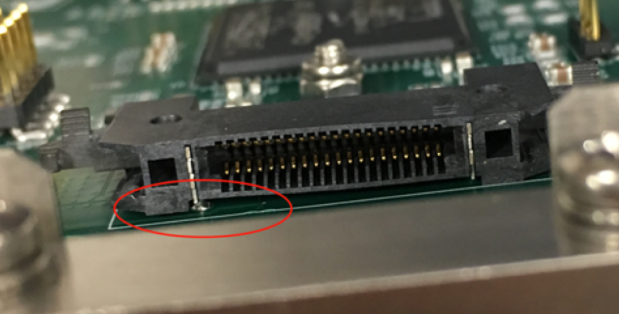
\includegraphics[width=0.85\linewidth]{sp-tpcelec-femb-problem.png}
\end{dunefigure}

\begin{comment}During the integration of the \dwords{femb} onto the \dword{apa}s 
and the cold tests that preceded the \dwords{apa} installation
inside the \dword{pdsp} cryostat a problem occurred %was observed 
on the 
connection between the cold readout and control cables and the
\dwords{femb}. In multiple cases the connector %is 
detached from
the \dword{femb} causing a loss of communication. 
\end{comment}
During the integration of the \dwords{femb} onto the \dword{apa}s 
and the cold tests that preceded the \dword{apa} installation
inside the \dword{pdsp} cryostat,  multiple connectors  
detached from
the \dword{femb}, causing a loss of communication.  
%For \dword{pdsp} w
We replaced the \dwords{femb} %This problem was fixed for 
on all the \dword{apa}s that had been tested in the cold box. % by replacing the \dword{femb}. 
One additional \dword{femb} was 
replaced on the \dword{apa} that had been installed without undergoing 
the test in the cold box. This %problem 
detachment may also be the cause
of the loss of the external clock signal on one of the \dwords{femb}
that was observed after cooldown. % of the detector. 
%
The problem 
with the connector has been traced to a mechanical interference between 
the \dword{pcb} of the \dword{femb} and the epoxy deposited as a protective measure on the small printed circuit
board to which the cold cables are soldered and which forms the 
male part of the connector. The height of the epoxy can cause 
the female part of the connector to lift from the \dword{pcb},
as shown in 
Figure~\ref{fig:pdsp-femb-connector}. %This problem is being 
%addressed by a redesign of the connection between the \dword{femb}
%and the cold cables, as discussed in 
Section~\ref{sec:fdsp-tpcelec-design-femb} discusses the redesign of the connection to address the problem.

\begin{dunefigure}
[Spectrum of the noise on the ProtoDUNE-SP APA wires]
{fig:pdsp-noise}
{Spectrum of the noise on the different \dword{pdsp} \dword{apa} wire planes before
(left) and after (right) applying a simple common-mode filter.}
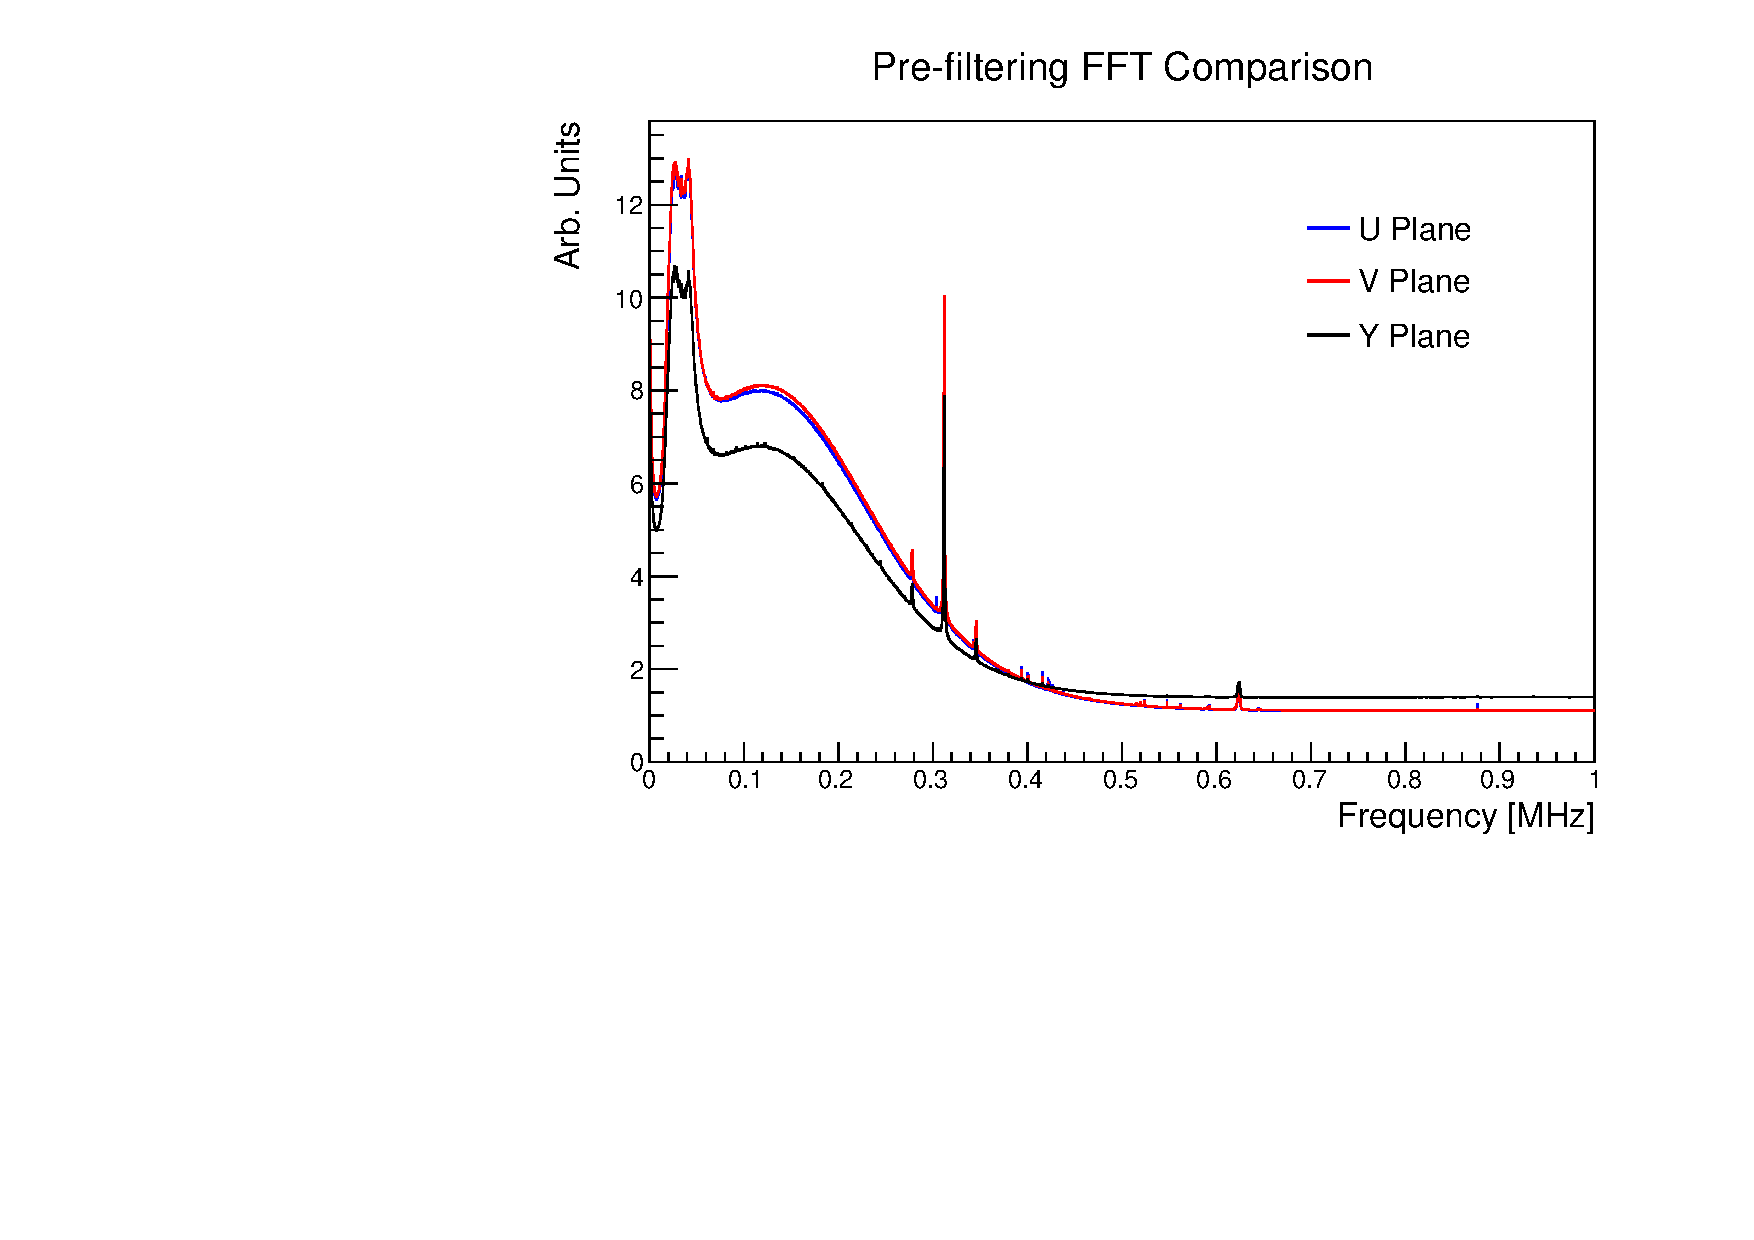
\includegraphics[width=0.49\linewidth]{sp-tpcelec-avgFFT-WithoutFilt.pdf}
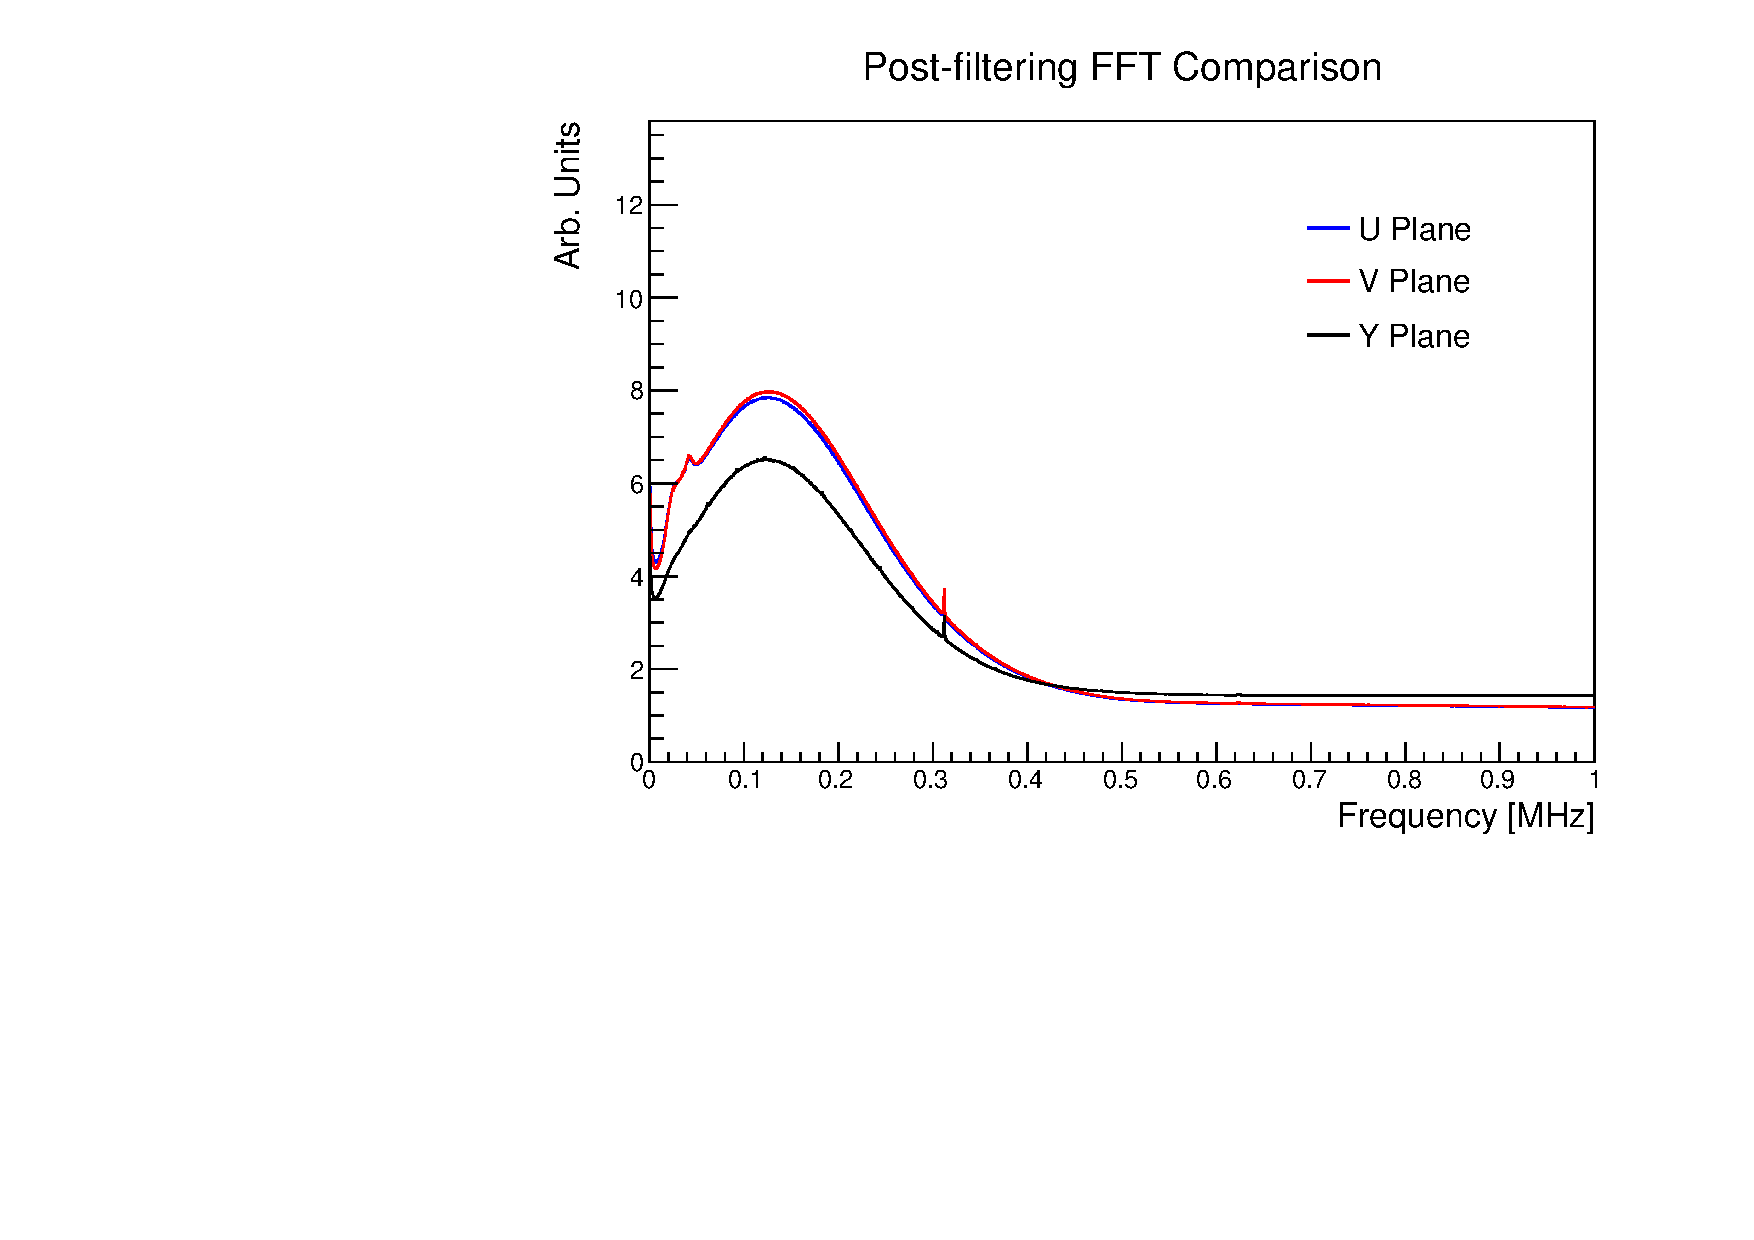
\includegraphics[width=0.49\linewidth]{sp-tpcelec-avgFFT-WithFilt.pdf}
\end{dunefigure}

Analysis of the \dword{pdsp} data is just starting, as of February 2019, and 
we will learn more about the detector and how its different components interact
from this data. The level of noise mentioned in Section~\ref{sec:fdsp-tpcelec-overview-pdune}
(approximately $\SI{550}{e^-}$ on the collection wires,
and approximately $\SI{650}{e^-}$ on the induction wires) 
was measured with raw data, without any
filtering or selection applied to the pulses on the \dword{apa}
wires. A simple common-mode filter can significantly reduce the 
noise, particularly at low frequencies, as shown in Figure~\ref{fig:pdsp-noise},  
a comparison of the noise spectrum on the three planes of the \dword{apa} 
before and after the filtering. The spectrum prior to the filtering shows 
a significant increase at frequencies $<$\SI{60}{kHz} that in \dword{microboone} 
had been associated with the low-voltage regulators that are installed
on the \dwords{femb}~\cite{Acciarri:2017sde}. This contribution to the noise 
has actually been significantly reduced compared to initial observations at 
\dword{microboone} thanks to RC filters that have been added
on the \dword{pdsp} \dwords{femb}. Further work is required to
understand why these RC filters do not suppress completely this
specific noise source, as indicated by tests performed in other setups.
The noise spectrum prior to the filtering also shows spikes at multiple 
discrete frequencies, and in some cases the noise sources have been 
identified (for example, cameras' operation inside the cryostat
contributes to the peaks at \num{310} and \SI{630}{KHz};
malfunctioning bias voltage supplies also contribute to the noise). We 
expect that further data analysis and tests with \dword{pdsp} 
will result in improvements to the \dword{tpc} electronics design that 
already demonstrates excellent performance.

%%%%%%%%%%%%%%%%%%%%%%%%%%%%%%%%%%%
\subsection{Remaining Design and Prototyping Tasks}
\label{sec:fdsp-tpcelec-overview-remaining}

 \dword{pdsp} was %has been 
 built with multiple
goals, one of which was to demonstrate that the specifications
for \dword{dune} could be met with a design that would only require a simple
scale up of the detector size. The data collected with \dword{pdsp}
in fall 2018 has demonstrated that noise levels well below the target
of \SI{1000}{e$^-$} can be achieved in \lar, validating the
detector system design approach planned for the \dword{dune} \dword{spmod}.

%Despite the success of \dword{pdsp} there are multiple areas where
Still, additional design and prototyping work is required in several areas before %the
%beginning of the 
the start of \dword{spmod} construction, with differing levels of risk and engineering work, as estimated in Table~\ref{tab:SPCE:designstatus}. % \dword{dune} detector construction. 
%These design changes can be ordered depending on the risk and the amount of engineering that is required. 
\begin{comment}
At one end of the spectrum is the change of the
design of the cryostat penetration, that in \dword{pdsp} housed one
\dword{ce} and one \dword{pds} flange in a tee-shape. For \dword{dune}
there will be two \dword{ce} flanges in addition to the \dword{pds}
flange, arranged in the shape of a cross. The increase of the number
of flanges may require some structural reinforcement and additional
finite element analysis simulations to estimate the proper flow of
argon to avoid any back-diffusion of oxygen into the cryostat in case
of leaks on the flanges and to ensure that the temperature gradient
in the argon is acceptable. In cases like this it can be easily
argued that the amount of engineering required to finalize the
detector design for \dword{dune} is minimal compared to the work already
done for past \dword{lar} detectors, starting with \dword{microboone} and
other prototypes, and finishing with \dword{pdsp}. \end{comment}
%
For example, changing the number and arrangement of cryostat penetrations to accommodate 
 two \dword{ce} flanges in addition to the \dword{pds}
flange can be considered relatively minimal. It may require some structural reinforcement and additional \dword{fea} simulations to estimate the proper flow of
argon so as to avoid any back-diffusion of oxygen into the cryostat in case
of leaks on the flanges and to ensure an acceptable temperature gradient in the \lar.
%
\begin{comment}At the opposite
side of the spectrum is the \dword{asic} design, with the
development of \dword{coldata}, \dword{cryo}, and of a completely new \dword{adc}
that is being designed to address the shortcomings of the \dword{bnl}-designed
P1-\dword{adc}, non-linearities, and stuck bits. In Table~\ref{tab:SPCE:designstatus}
we describe our estimate of the amount of work required to complete
the design and prototyping of the \dword{tpc} electronics detector components for
\dword{dune}. In this table we consider only the amount of engineering time 
required to complete the design of the various detector components. Later 
in this Section we analyze the risk that the design
and prototyping of these components could affect the \dword{dune} detector
construction schedule.\end{comment}
%
On the other hand, the \dword{asic} design, with the
development of \dword{coldata} and of a completely new \dword{adc} is more involved. 

\begin{dunetable}
[Status of the design of the different CE detector components]
{p{0.27\textwidth}p{0.15\textwidth}p{0.50\textwidth}}
{tab:SPCE:designstatus}
{Status of the design of the different CE detector components and expected
amount of engineering and prototyping required prior to construction.}
Component & Status & Expected work \\ \toprowrule
\dword{larasic} & Advanced & Fix issues observed in \dword{pdsp}, port differential output from \dword{coldadc} design \\ \colhline
Commercial ADC & Complete & None \\ \colhline
\dword{coldadc} & \multicolumn{2}{l}{See text for details} \\ \colhline
\dword{coldata} & \multicolumn{2}{l}{See text for details} \\ \colhline
\dword{cryo} & \multicolumn{2}{l}{See text for details} \\ \colhline
\dword{femb} & Advanced & Experience with multiple prototypes, final design will follow the \dword{asic} selection \\ \colhline
Cold cables & Very advanced & Minor modifications, additional vendor qualification \\ \colhline
Cryostat penetrations & Advanced & Add \dword{ce} flange for bottom \dword{apa} \\ \colhline
\dword{wiec} & Very advanced & Add air filters and hardware interlock system \\ \colhline
\dword{wib} & Advanced & Update design to use cheaper FPGA, modify \dword{femb} power, new firmware \\ \colhline
\dword{ptc} & Very advanced & Add interface to interlock system \\ \colhline
Power supplies & Very advanced & Investigate possible additional vendors, rack arrangement \\ \colhline
Warm cables & Very advanced & Finalize cable layout, identify vendors \\ \colhline
Readout and control fiber plant & Very advanced & Finalize plant layout \\ \colhline
\end{dunetable}

The area that requires most work is that of the \dword{asic}s that are mounted
on the \dwords{femb}. \dword{larasic} has already gone through eight design
iterations, the last three directly targeted for \dword{dune}, and has already been used, 
in one of its versions, for \dword{microboone} and for \dword{pdsp}, where it has reached the 
noise levels specified for the \dword{dune} \dword{spmod}. At least one additional design iteration is
required to address the issues observed during the \dword{pdsp} operations and
to implement a single-ended to differential converter to improve the interface
with the newly developed \dword{coldadc}. To ensure the success of the next 
design iteration we are investing in the development of appropriate transistor
models for the \SI{180}{nm} \dword{cmos} technology for operation in \lar, such that the saturation effect observed in 
\dword{pdsp} can be properly addressed first in simulation and then with improvements 
in design. It should be noted that so far approximate models, originally developed for 
the same \SI{180}{nm} technology, but with different design rules, have been used for 
the \dword{larasic} development, and therefore it should not be a surprise
that the \dword{larasic} may have limitations in some corner of the phase space.
The circuitry for the single-ended to differential converter has already been 
developed in the \SI{65}{nm} technology and needs to be ported to the \SI{180}{nm}
technology used for \dword{larasic}. We consider that appropriate measures have been
put in place to minimize the risk associated with the need of a further
prototyping iteration. Nevertheless, in Section~\ref{sec:fdsp-tpcelec-risks-design}
we consider a generic risk for a delay in the availability of \dword{asic}s and
argue that this delay would not have an impact on the beginning of \dword{dune} operations.

It should be noted that even if the baseline for \dword{spmod} foresees the usage
of custom \dwords{asic} for the \dword{adc} and the data serialization, we should
note that a solution based on commercial components is available and has been 
demonstrated to work by the \dword{sbnd} collaboration. This solution is based on
the use of a \dword{cots} \dword{adc} and an \dword{fpga} for the data serialization,
and further validation is planned for spring 2019. We consider this solution as
a fall-back solution for \dword{dune}. Custom solutions for the \dwords{asic} are 
being developed to simplify the \dword{femb} assembly and reduce the power dissipated by the
electronics in the \lar.

The baseline solution for the \dword{adc} and the data serialization is based on two new 
\dword{asic}s, \dword{coldadc} and \dword{coldata}.
The first iteration of the \dword{coldadc} was submitted for fabrication
at the end of October 2018, and the chips were delivered in January 2019.
Initial results from the tests of the \dword{coldadc} prototypes have
been discussed in Section~\ref{sec:fdsp-tpcelec-design-femb-adc}. The
results obtained so far are encouraging, despite the fact that some
flaws have been identified in the design. Even if one additional design
iteration is required, we think that the status of \dword{coldadc} can
be characterized as having reached the ``Advanced'' status.

We are also considering an alternative solution for the readout, where
the three \dword{asic}s are replaced with a single one, the \dword{cryo}
chip that is going through a development that is proceeding with a 
timeline similar to that of \dword{coldadc}. Also in this case the
chips from the first submission have been delivered in January 2019.
Initial results from the tests of the \dword{cryo} prototypes have
been discussed in Section~\ref{sec:fdsp-tpcelec-design-femb-alt-cryo}.
Like in the case of \dword{coldadc}, the results obtained so far are
encouraging, despite the problem observed with the digital multiplexer.
Depending on the performance of the \dword{asic}, \dword{cryo} should
also be characterized as having reached the ``Advanced'' status.

The first complete prototype of \dword{coldata} was submitted in 
April 2019, with the delivery of chips expected for July 2019.
The design of this first complete prototype builds on the success of
the first partial prototype (CDP1) that was fabricated and tested in 2017.
This first prototype included the control registers inside the 
\dword{asic}, the \dword{i2c} interface required to program and read-out
the status of these registers, the \dword{spi} interface required to
configure \dword{larasic}, the phase-lock loop required to generate
clocks internal to the chip, the data serializer, and a current-mode
line driver. The transition to the first complete prototype
involves the addition of interfaces to the \dword{coldadc} (\dword{uart}
and \dword{i2c}), an additional \dword{i2c} interface to allow programming two
\dword{coldata} \dword{asic}s on the same \dword{femb}, and the
addition of a line-driver with pre-emphasis required for operation
with long cables (up to \SI{22}{m}) in \lar. The same design and
validation methodology used for the CDP1 prototype and the \dword{coldadc}
is being used. This should guarantee that after the tests done in
summer 2019 \dword{coldata} will reach the ``Advanced'' design 
status. 

There have already been multiple iterations of \dwords{femb} that
have been fabricated and tested and used for data taking in 
\dword{microboone} and in \dword{pdsp}. The \dword{sbnd} Collaboration
is starting the production of \dwords{femb} based on the commercial \dword{adc} and
\dword{fpga} solution. The design of the \dword{femb} needs to be adapted
for the different \dword{asic} solutions that are being considered
for \dword{dune}. This development is already ongoing, as system tests 
where the \dwords{femb} are connected to an \dword{apa} are part
of the qualification tests. The design status for the \dword{femb}
is already at the ``Advanced'' level, and it will reach the 
``Very advanced'' level at the time of the \dword{asic}
selection. At that point only minor modifications may be
required. 

The only other \dword{tpc} electronics detector components that do not yet
reach the ``Very advanced'' level are the cryostat penetrations, as
discussed above, and the \dword{wib}, where small
design changes will be done prior to production to use a more
modern and cheaper \dword{fpga}. Additional changes will be required to
the power distribution scheme, since the number of power lines
and the corresponding voltages will be reduced compared to
\dword{pdsp}. The transition to a more modern \dword{fpga} will allow 
more extensive data monitoring inside the \dword{wib}, but may
also require developing new software and porting the firmware
from one family of \dword{fpga}s to another. 

For all other detector components the estimate of the design
maturity is considered ``Very advanced'' based on the experience
gained with commissioning and operation of \dword{pdsp}. The 
cold signal cables will be modified to reduce the number of
connections and to address the issues observed with the connector
on the \dword{femb}. The design of the \dword{wiec} needs to
be modified to include air filters to minimize the possible
damage from dust and/or chemical residues from  explosives 
during the lifetime of the experiment at \dword{surf}.
The \dword{ptc} is going to be modified to add an interface to
the hardware interlocks of the detector safety system. For
cables and fibers on the top of the cryostat the only work that
remains to be done is the design of the actual cable plant, 
which will then fix the length of the cables. The arrangement
of power supplies in the racks on top of the cryostat is the
only other remaining design task. For many components the
qualification of additional vendors could also be considered
as part of value engineering, to reduce the risks of vendor
lock-in and to minimize costs. 

